\chapter{Controller Design}
This chapter follows the stages of designing a controller for a quadrotor and begins by discussing the overall strategy. An analysis of existing rotorcraft control systems has been done in Section \ref{SECT_ControlReview}. The system must be able to follow waypoint commands, containing a position reference in the North, East and Down frame. As well as align with a desired heading, this reference will be in the form of a Euler angle. The detailed design goals are discussed before the controller design is begun.

\section{Design Goals}
The design goals for the controller system are presented here. The controllers must ensure that the system is capable of meeting all of the prescribed requirements.

\begin{enumerate}
	\item The controller must be able to track a position reference in the North, East and Down frame. The limited space in which the vehicle must fly requires a final system with sufficient damping and minimal overshoot.
	\item The transient response of the velocity control system must be rapid to ensure fast responses to changing setpoints caused by unexpected obstacles.
	\item The controller's must be robust to unmodelled system errors. To accomplish this sufficient phase margin is required to handle unmodelled timing delays and sufficient gain margin is required to handle unmodelled errors in actuation and plant gains.
	\item The output of the controllers must never exceed the thrust capabilities of the system. 
	\item The controllers should be designed as to not demand large angles for the craft.
	\item The velocity of the craft must be limited for flight inside a confined environment.
	\item The controllers must be capable of rapidly rejecting disturbances.
	\item The designed controller bandwidth must not exceed the bandwidth capable of the rotor motor system.
\end{enumerate}

The stipulated design goals are appropriate for a vehicle expected to fly in a confined space and differ from traditional flight which requires high speed and fast position tracking.

\section{Flight Control Strategy}
Figure \ref{IM_ControlStrategy} represents the high level control strategy for this project. This discussion will break the system into three main components: an altitude controller, a horizontal flight controller and a heading controller.	

The altitude controller starts by getting a position reference in the earth frame. This reference is fed through a Proportional Integral (PI) controller to create a desired climb rate. The climb rate reference is converted into the body frame and is then controlled using a Proportional (P) controller to produce a body acceleration reference. The heave controller can only produce a force perpendicular to the rotor, thus the Z-Axis acceleration component is taken and fed through an additional PI heave controller. The output of this inner heave controller would be the virtual actuator $\delta_Z$.

The horizontal controller gets both a North and an East position reference and uses PI controllers to create velocity setpoints in the earth frame. These setpoints are converted to the body frame where the linear velocity P controller works and outputs acceleration references in the body frame. Using the body acceleration references, roll and pitch rate setpoints can be created using a tilt angle controller. These rate set points are fed into the inner rate loop lead lag controllers which output the virtual actuators $\delta_\phi$ and $\delta_\theta$.

Lastly the heading controller is discussed. Correct design of the tilt angle controller will decouple the vehicle's horizontal controller from a dependency on the heading of the craft. This allows seamless implementation of a heading controller. The heading controller is broken down into two parts: a yaw angle and a yaw rate controller. The angle loop uses a PI control architecture while rate loop utilises a simple P controller. The output of the yaw rate controller is the virtual actuator $\delta_\psi$.

\begin{figure}[H]
 	\centering
 	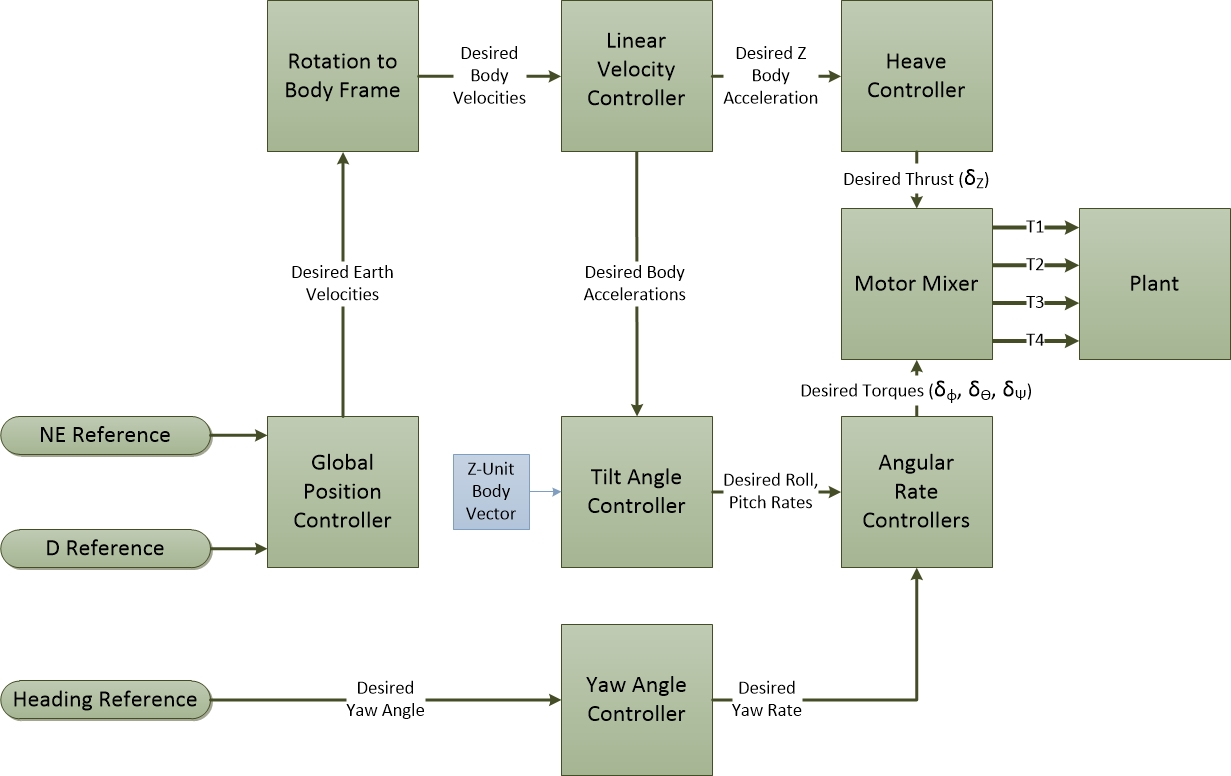
\includegraphics[height = 10cm]{../References/Diagrams/HighLevel.jpg}
 	\caption{High Level Control Strategy}
 	\label{IM_ControlStrategy}
\end{figure}

Each controller utilises the same rotor system to produce their outputs. This dependency on a single generation system allows for interference between the controllers. To ensure that no loop can saturate another, each system is given a percentage of headroom in which it can work, as shown in Table \ref{tab:HeadRoomPercentages}. The controller design must ensure that the thrust commanded during a step response is within those limits.

\begin{table}[H]
 	\centering
 	\begin{tabular}{l | c | c |}
 		Controller 				& Percentage & Allowed Thrust Per Rotor\\
 		\hline\hline
 		Altitude 	   			& 64\% & 12.16N	\\
 		North  		    		& 8\%  & 1.52N	\\
 		East					& 12\% & 2.28N	\\
 		Heading 		    	& 6\%  & 1.14N	\\
 		Safety Factor 			& 10\% & 1.9N   \\
 	\end{tabular}
 	\caption{Thrust Headroom Controller Percentages}
 	\label{tab:HeadRoomPercentages}
\end{table}
	 
\section{Altitude Controller}
This section discusses the design and implementation of the altitude controller which is responsible for controlling the desired height of the craft. The craft is required to fly in confined spaces and must be able to track a setpoint with zero steady state error and negligible overshoot. In order for the altitude system to handle disturbances, an integrator term will be required. The system must be able to respond quickly to commands, however it must not exceed it's thrust utilisation percentage. To do this the system will require an upper limit which should not be reached. A lower limit is then introduced so the craft does not descend too quickly.

The overall altitude controller is structured as a set of cascaded control loops, with the most inner loop controlling the aircraft's acceleration and the most outer loop controlling the desired altitude in the earth frame. The system must be able to respond to disturbances quickly. Therefore, the inner heave loop utilises a PI controller to follow a desired vertical acceleration reference. The climb rate P controller is responsible for generating these acceleration references and is fed a desired linear vertical velocity reference by the altitude hold P controller. In order to reject measurement errors in the inner loops, the altitude hold controller makes use of a limited integrator that does effect the bandwidth of the system. Before the controller's can be designed, an analysis of the system's heave dynamics must first be performed.
	 
	 \subsection{Heave Dynamics}
	 Using Newton mechanics at near hover conditions for the aircraft, the heave dynamics can be derived and are shown in \eqref{EQ_HeaveNewton}. Where $\dot{W}$ is the current acceleration of the craft in the Z-Axis and $m$ is the vehicles's mass. $Z$ is defined as the current instantaneous force being produced by the rotors.
	 
	 \begin{equation}
	 \label{EQ_HeaveNewton}
	 \dot{W} = \dfrac{Z}{m}
	 \end{equation}
	 
	 The state variable of the system is chosen as $Z$ with the output of this plant being $\dot{W}$. Using the transfer function for motor-rotor lag dynamics seen in \eqref{EQ_MotorDelay} and the dynamics seen in \eqref{EQ_HeaveNewton}, the state space equation for the system can be derived and is shown in \eqref{EQ_HeaveStateSpace1} and \eqref{EQ_HeaveStateSpace2}. 
	 
	 \begin{eqnarray}
	 [\dot{Z}] &=& - [\dfrac{1}{\tau}] \ [Z] + [\dfrac{1}{\tau}] [\delta_Z]\label{EQ_HeaveStateSpace1}\\\label{EQ_HeaveStateSpace11}
	 [\dot{W}] &=& - [\dfrac{1}{m}] \ [Z]\label{EQ_HeaveStateSpace2}
	 \end{eqnarray}
	 
	 Subsequently the transfer function can be calculated and the result is shown in \eqref{EQ_HeaveTF}. The negative gain of the transfer function must be noted and is caused by the direction of the defined axes, with the rotors producing a negative Z-Axis force.
	 
	 \begin{equation}
	 G(s)_{heave} = \frac{\frac{-1}{m \times \tau}}{s + \frac{1}{\tau}}\label{EQ_HeaveTF}
	 \end{equation}
	 
	 The rotor motor lag of $0.125$\,s stipulated in the system identification chapter produces the pole at $\dfrac{-1}{\tau} = -8$ and indicates the maximum response capabilities and timing constant of the rotor system.
	 
	 \subsection{Heave Controller}
	 The heave controller is responsible for commanding the $\delta_Z$ virtual actuator to achieve a desired Z-Axis acceleration in the body frame. The heave controller is the fastest controller in the altitude system and should utilise as much bandwidth as the rotor-motor system allows. The altitude controller wishes to reject disturbances quickly and thus a PI architecture was initially chosen as shown in Figure \ref{IM_HeaveController}. The system should be stable and exhibit a reasonable phase margin and therefore be able to compensate for margin loss when the outer loops are closed. The phase margin in the open loop system should at least $70$\textdegree.
	 
	 The integrator is used to reject disturbances, while the most left limiter shown in Figure \ref{IM_HeaveController} was added to stop integrator wind up and is not considered during the linear controller design. The proportional gain is used to move the closed loop poles and achieve the desired bandwidth. The dynamic response of the system can be investigated using the root locus and bode plots shown in Figure \ref{IM_HeaveControlRoot} and \ref{IM_HeaveControlBode}. 
	 
	 \begin{figure}[H]
	 	\centering
	 	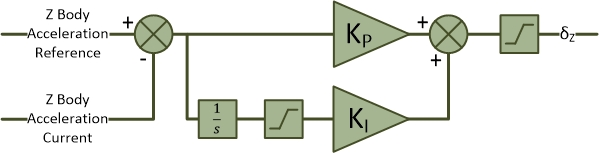
\includegraphics[height = 3.5cm]{../References/Diagrams/HeaveController.jpg}
	 	\caption{Heave Controller -  Control Diagram}
	 	\label{IM_HeaveController}
	 \end{figure}
	 
	 Figure \ref{IM_HeaveControlRoot} shows the root locus of the system with the PI controller included. The controller introduces a new open loop pole at the origin. To maintain a first order response, the zero is placed close to the plant pole. This placement will attenuate the open loop, plant pole's response. Finally the gain is varied until the closed loop responses are closely aligned with the naturally occurring open loop pole. The final closed loop poles are a set of complex poles and are located at $-7.55 \pm 3.64 i$. The frequency response can be evaluated using the bode plot in Figure \ref{IM_HeaveControlBode}. 
	 
	 \begin{figure}[H]
	 	\centering
	 	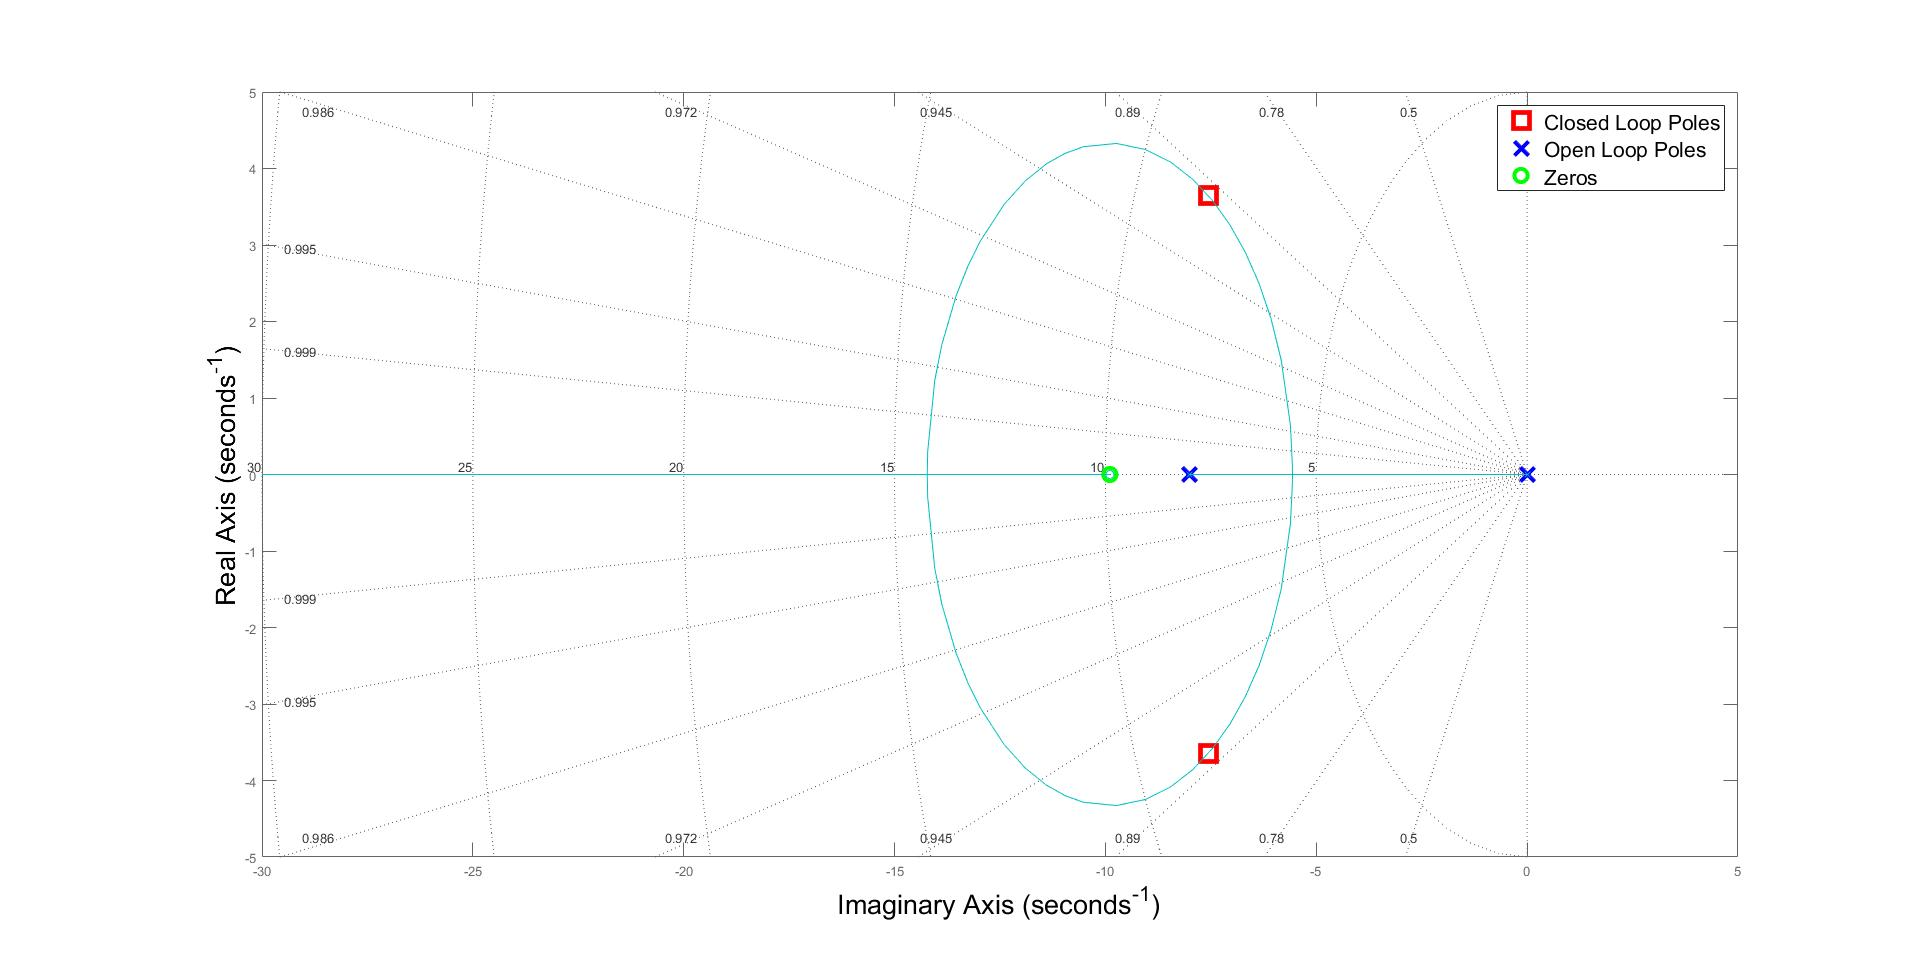
\includegraphics[height = 7.9cm]{../Design/Matlab/Controllers/heave_root.jpg}
	 	\caption{Heave Controller -  Root Locus}
	 	\label{IM_HeaveControlRoot}
	 \end{figure}
	 
	 The final cross over frequency is shown on the bode plot for the heave controller in Figure \ref{IM_HeaveControlBode}. The gain plot shows the controller adjust the crossover frequency to $7.99$\,rad/s which is close to the limit of the system. The controller also increases the phase of the system and has a final phase margin of $84$\textdegree.
	 
	 \begin{figure}[H]
	 	\centering
	 	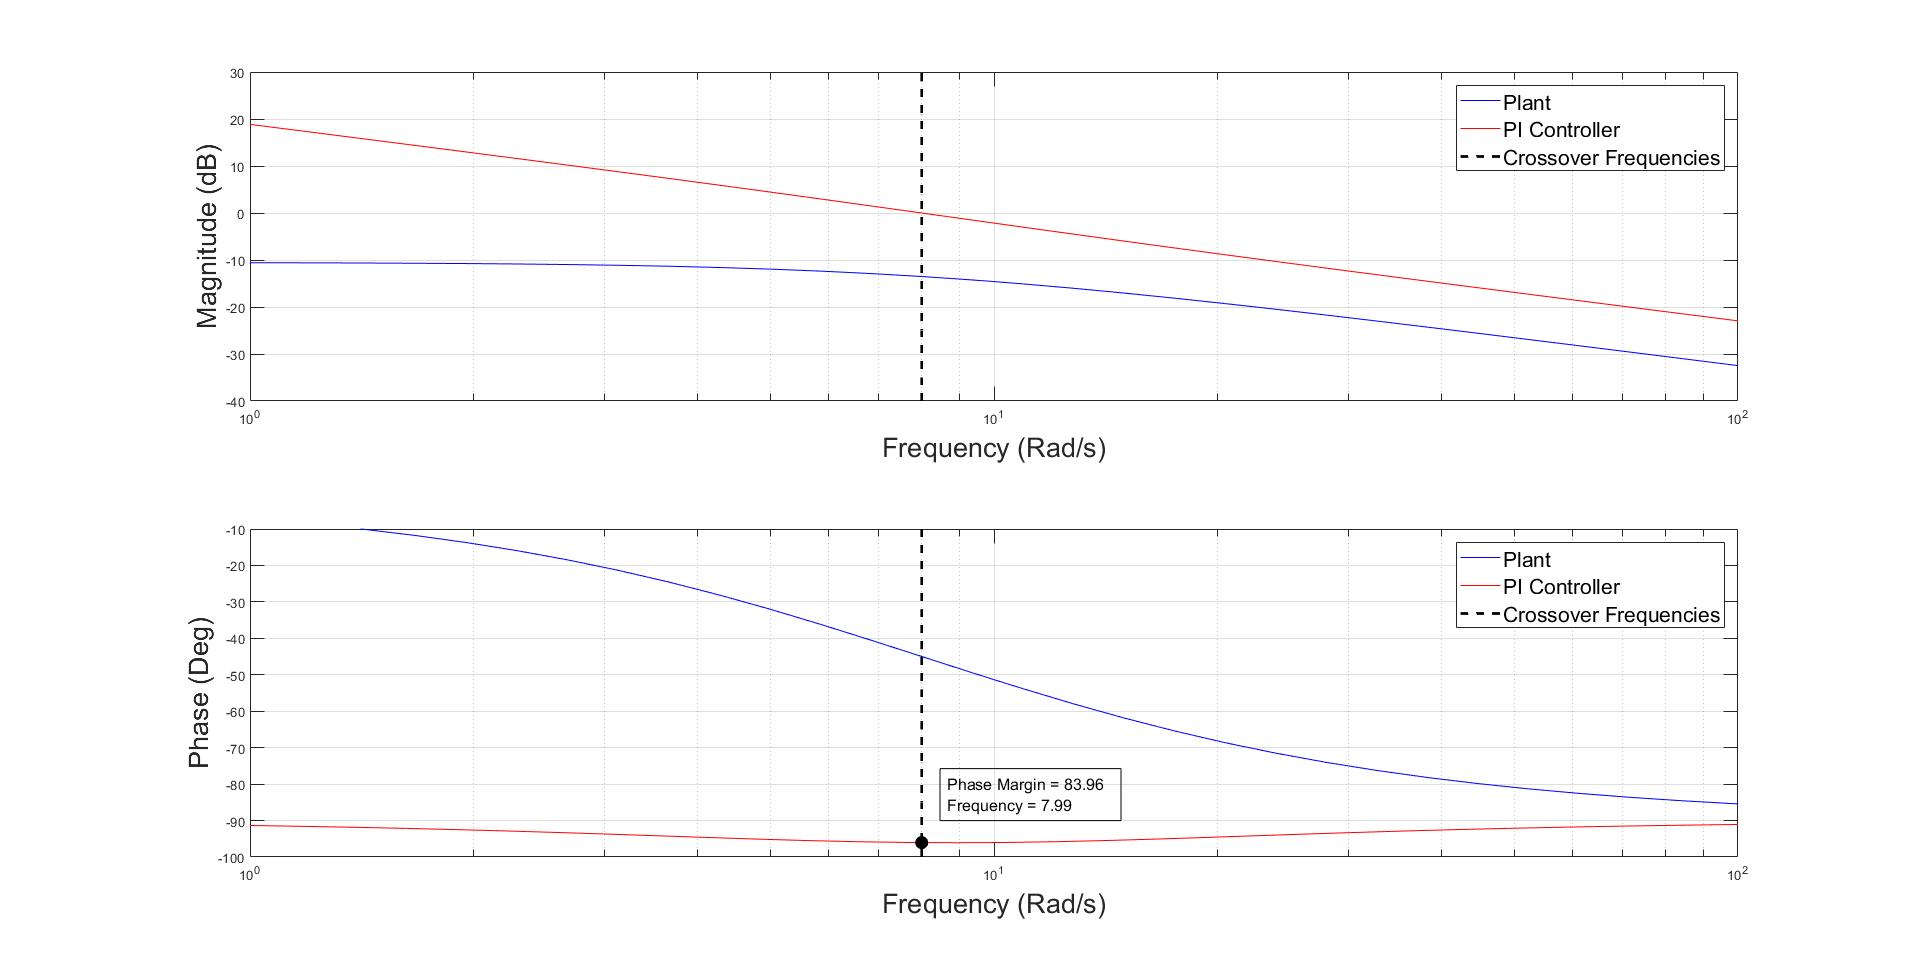
\includegraphics[height = 7.9cm]{../Design/Matlab/Controllers/heave_bode.jpg}
	 	\caption{Heave Controller -  Bode Plots}
	 	\label{IM_HeaveControlBode}
	 \end{figure}
	 
	 An additional non linear element in the form of a limiter is brought into the system to limit the maximum and minimum thrust commands. The maximum limit is used to ensure the heave controller does not saturate the motors, thereby creating headroom for the angular rate controllers. The lower limit is used to ensure the vehicle always descends at a steady pace. The maximum thrust allowances are displayed in table \ref{tab:HeadRoomPercentages}, the final limits chosen are shown in Table \ref{tab:HeaveLimits}.
	 
	 \begin{table}[!]
	 	\centering
	 	\begin{tabular}{l | c | c |}
	 		Limit Name 				& Min & Max\\
	 		\hline\hline
	 		Integrator Wind Up 	   	& -1.5 	& 1.5 \\
	 		Thrust Command 		    & 10	& 48.64 \\
	 	\end{tabular}
	 	\caption{Heave Controller Limits}
	 	\label{tab:HeaveLimits}
	 \end{table}
	 
		 \subsubsection{Heave Controller Discussion}
		 Now that the system presents stable dynamic results in the frequency and Laplace domains, using the non-linear simulation, the time domain responses can be discussed in brief. The resultant step response, including the PI controller, is shown in Figure \ref{IM_HeaveStepDist}. To demonstrate the disturbance rejection capabilities of the design, a force of $10N$ is applied to the drone at $2.5s$.
		 
		 \begin{figure}[H]
		 	\centering
		 	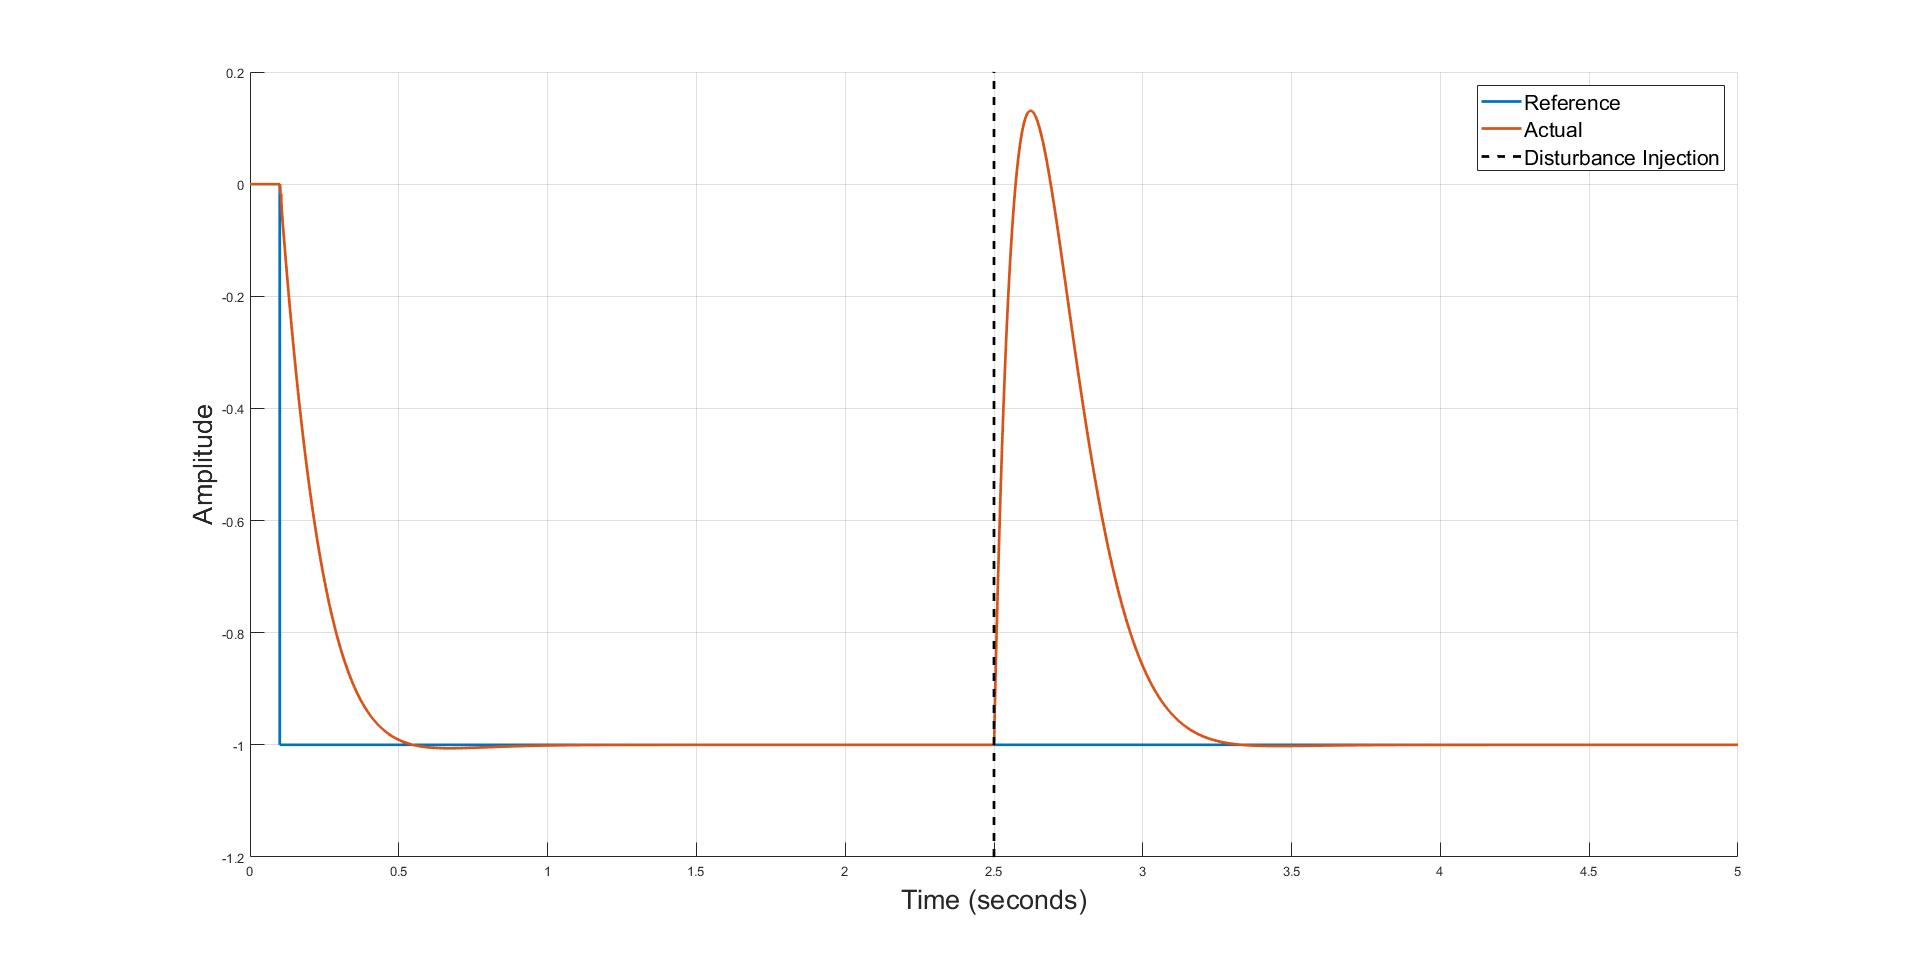
\includegraphics[height = 7.9cm]{../Design/Matlab/Controllers/heave_step.jpg}
		 	\caption{Heave Controller -  Step Response}
		 	\label{IM_HeaveStepDist}
		 \end{figure}
		 
		 The heave controller, as the most inner loop, limits the response for the rest of the altitude control system. The proposed design brings the heave loop response close to the limits of the plant, thus producing a similar (but slower) timing constant to that of the motor-rotor system. The system reaches and settles within 5\% of the reference by $0.31s$, is critically damped and presents negligible overshoot. The system also shows to be capable of tracking an acceleration setpoint with zero steady state error. As shown in Figure \ref{IM_HeaveStepDist} the system can also respond quickly to a large, sudden and constant disturbance. The maximum rotor thrust commanded during this run is $3.35$\,N. 
		 Gravity will add on offset of $mg$ to the acceleration setpoint, this needs to be rotated into the body frame as this controller provides force in the Z-Body Axis. 
	 
	 \subsection{Climb Rate Controller}
	 The climb rate controller is responsible for controlling the vertical velocity of the aircraft, in the earth frame. This introduces the need for rotating either the reference or the command into the body frame. The decision can be made by considering the frame in which the sensing information is provided. Most aircraft make use of some form of global positioning system and using differentiation can calculate speed. However, due to the application environment, this aircraft will most likely use a velocity measurement sensor relative to the body frame. The architecture for the climb rate controller is outlined in Figure \ref{IM_ClimbRateControlLoop}. 
	 
	 \begin{figure}[H]
	 	\centering
	 	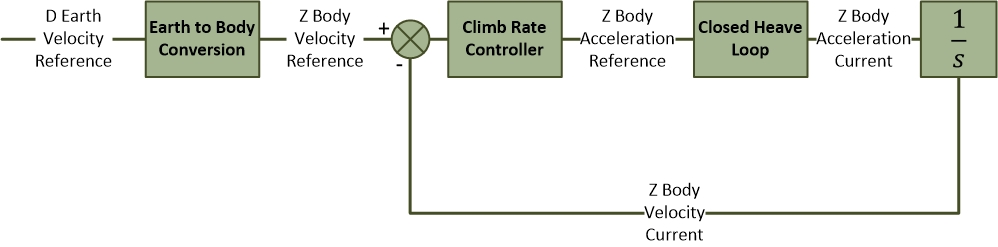
\includegraphics[height = 3.75cm]{../References/Diagrams/ClimbRateLoop.jpg}
	 	\caption{Climb Rate Controller Closed Loop}
	 	\label{IM_ClimbRateControlLoop}
	 \end{figure}
	 
	 At near hover conditions the plant can be linearised and the rotation can be excluded. Figure \ref{IM_ClimbRateController} shows the simplified climb rate controller architecture. The computational time required for rotating the references can be considered by ensuring the controller design provides a reasonable phase margin. The speed of the climb rate controller is limited by the inner heave leave control loop. The controller must react quickly but there must still be a sufficient bandwidth ratio between the inner and outer loop. The controller must be able to track a setpoint with zero steady state error, but is not required to reject disturbances. The craft is required ot produce a steady approach to position targets, the climb rate controller should then exhibit a damped first order response.
	 
	 \begin{figure}[H]
	 	\centering
	 	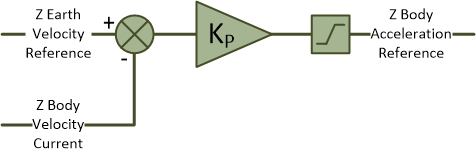
\includegraphics[height = 3.5cm]{../References/Diagrams/ClimbRateController.jpg}
	 	\caption{Climb Rate Controller}
	 	\label{IM_ClimbRateController}
	 \end{figure}		
	 
	 The open loop poles of the climb rate system are located at the closed loop pole positions of the inner heave system, while the mathematical relationship between acceleration and velocity yields an additional open loop pole at the origin. The free integrator in the plant ensures the system will track a step response with zero steady state error while the proportional gain is used to speed up the system and achieve the desired bandwidth. The dynamic response of the system is evaluated using the root locus and bode plots shown in Figure \ref{IM_ClimbRateRoot} and \ref{IM_ClimbRateBode}.
	 
	 \begin{figure}[H]
	 	\centering
	 	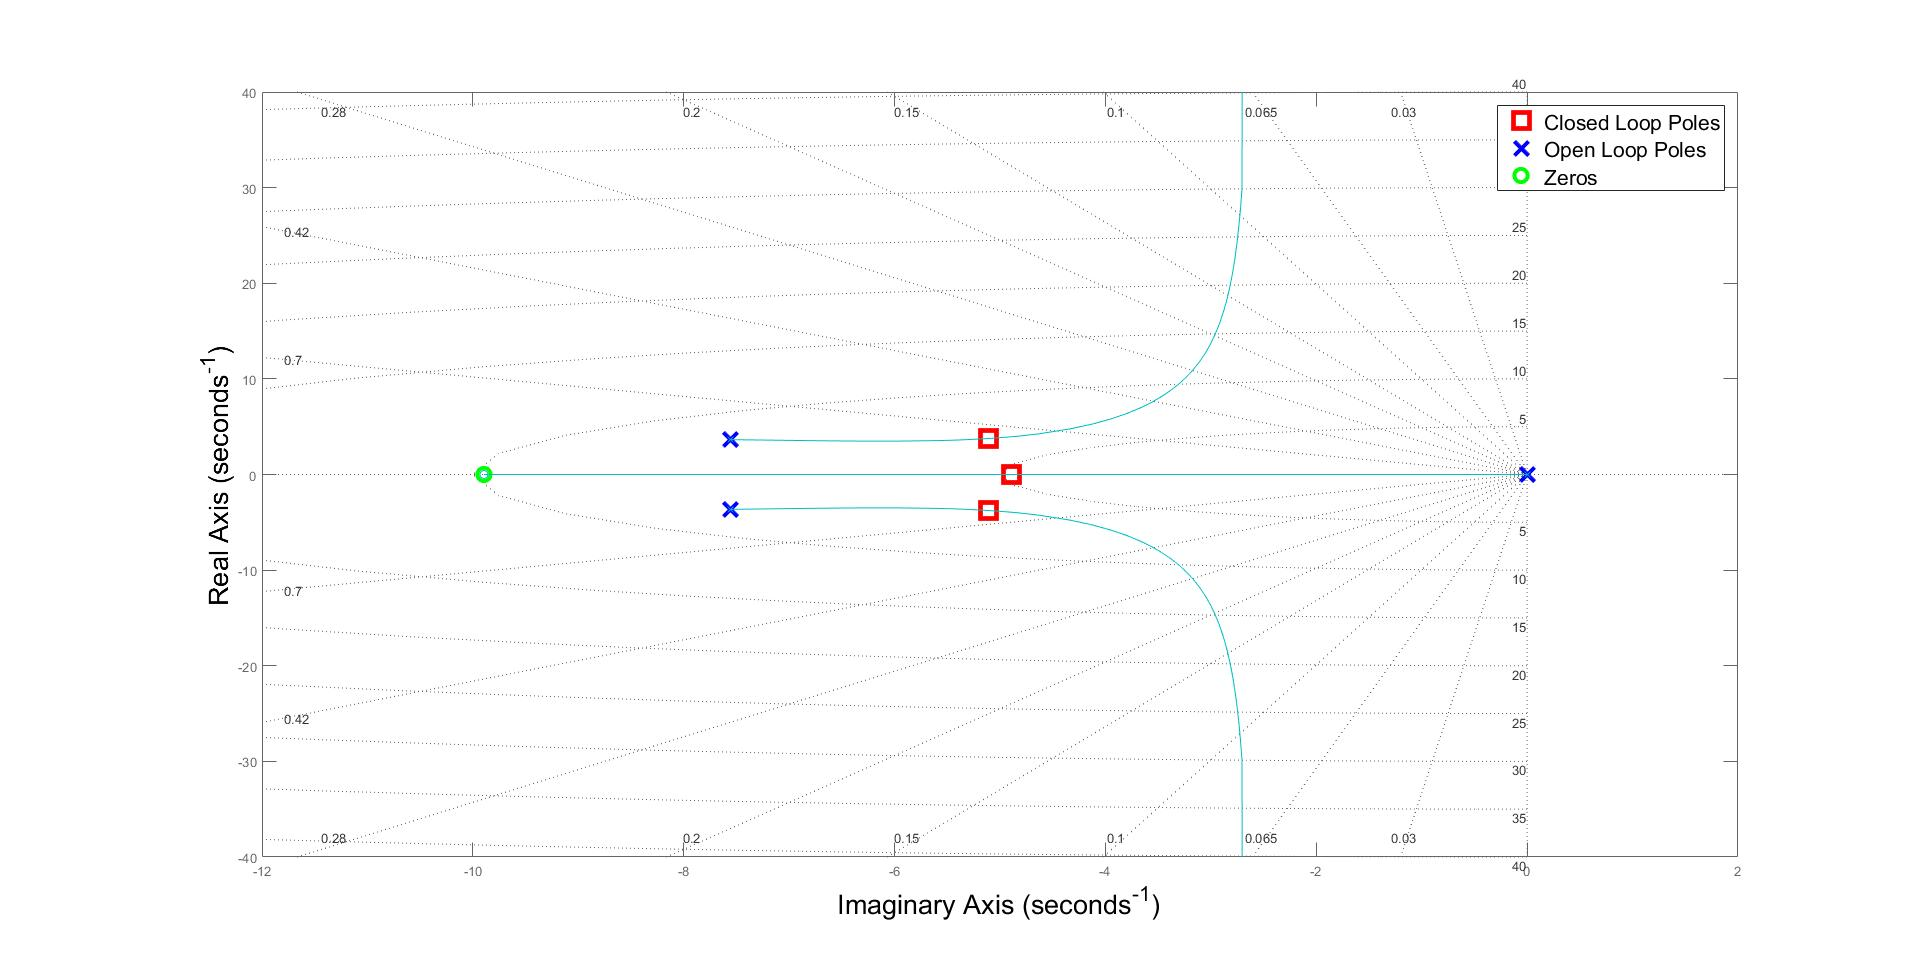
\includegraphics[height = 7.9cm]{../Design/Matlab/Controllers/climb_rate_root.jpg}
	 	\caption{Climb Rate Controller -  Root Locus}
	 	\label{IM_ClimbRateRoot}
	 \end{figure}
	 
	 Figure \ref{IM_ClimbRateRoot} shows the location of the three final closed loop poles. There is a non dominant complex pair which is placed at $-5.11 \pm 3.76i$. The dominant pole is critically damped and located on the imaginary axis at $-4.89$.
	 
	 \begin{figure}[H]
	 	\centering
	 	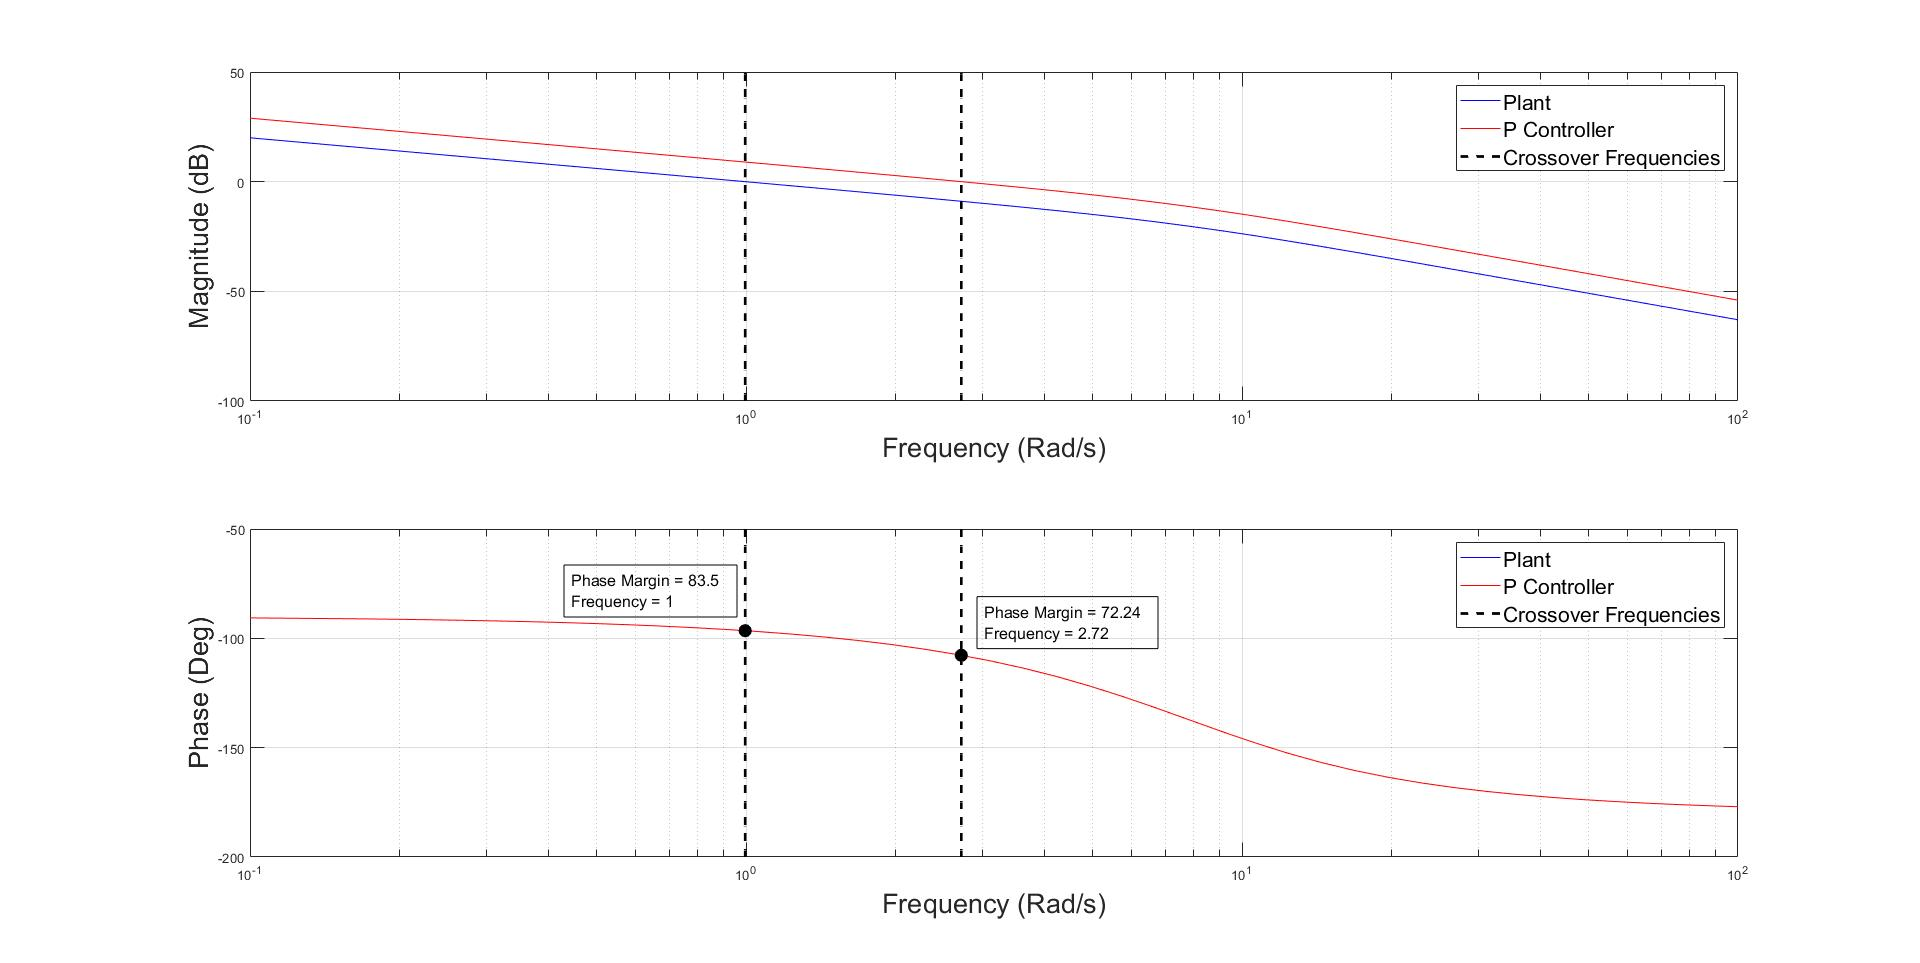
\includegraphics[height = 8cm]{../Design/Matlab/Controllers/climb_rate_bode.jpg}
	 	\caption{Climb Rate Controller - Open-Loop Bode Plots}
	 	\label{IM_ClimbRateBode}
	 \end{figure}
	 
	 The bode plot shown in \ref{IM_ClimbRateBode} shows zero change in phase due to the controller architecture. The gain however is increased and moves the crossover frequency to $2.72$\,rad/s. The ratio of inner and outer loop crossover frequencies is then $2.91$, providing enough bandwidth between the inner and outer loops. The phase margin can then be calculated to be $72$\textdegree. 
	 
	 As shown in Figure \ref{IM_ClimbRateController} there is a limiter applied to the acceleration commands. This limit is present due to the confined operational environment and ensures that the climb rate controller does not saturate the horizontal velocity controllers. The final limits are shown in Table \ref{tab:ClimbrateLimits}
	 
	 \begin{table}[!]
	 	\centering
	 	\begin{tabular}{l | c | c |}
	 		Limit Name 						& Min & Max\\
	 		\hline\hline
	 		Acceleration Command 		    & $-4m/s^{2}$ & $4m/s^{2}$ \\
	 	\end{tabular}
	 	\caption{Climb Rate Controller Limits}
	 	\label{tab:ClimbrateLimits}
	 \end{table}
	 
		 \subsubsection{Climb Rate Controller Discussion}
		 The dynamic response shows sufficient phase margin to handle unmodelled timing delays. While the ratio between the inner controller ensures this controller will not be influenced by the inner loop. The step response of the closed loop system is shown in Figure \ref{IM_ClimbRateStep}. The system has a $5$\% settling time of $0.747s$ and shows negligible overshoot. At $5s$ a disturbance of $10N$ is placed on the rotors and the system demonstrates the ability to continue tracking the desired setpoint with zero steady state error.
		 
		 \begin{figure}[H]
		 	\centering
		 	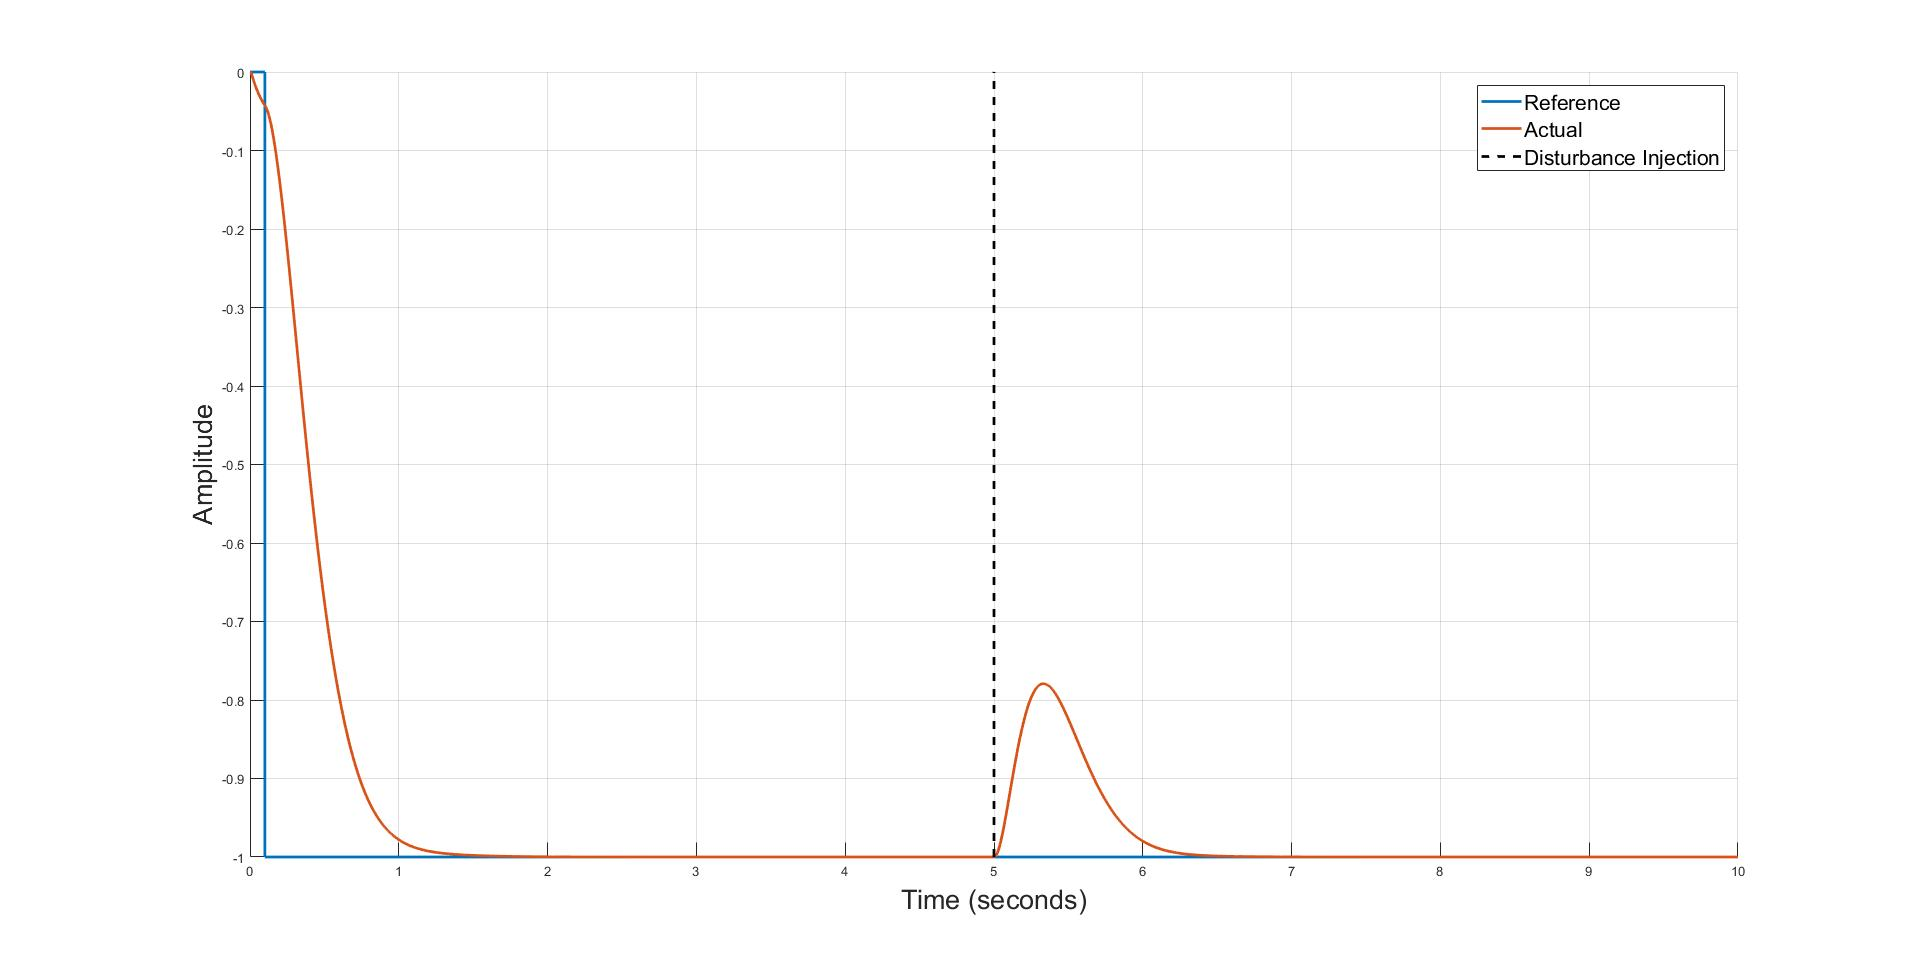
\includegraphics[height = 8cm]{../Design/Matlab/Controllers/climb_rate_step.jpg}
		 	\caption{Climb Rate Controller -  Step Response}
		 	\label{IM_ClimbRateStep}
		 \end{figure}
	 
	 \subsection{Altitude Hold Controller}
	 The final stage of the vertical control system is the altitude hold controller. This controller receives a desired altitude in the earth frame and outputs a reference velocity, also in the earth frame. The closed control loop block diagram is shown in Figure \ref{IM_AltHoldControlLoop}. 
	 
	 The altitude hold controller must be able to reject measurement errors in the inner loops, this can be achieved by adding an integrator into the controller. The system must also be able to track a set point with zero steady state error and must show a damped response with little overshoot. The system must be able to react quickly to commands, but is limited by the bandwidth of the climb rate system. The final bandwidth of this loop must be such that this controller is not influenced by the inner climb rate loop. To ensure this, the altitude controller should be a magnitude of at least 2 smaller than the climb rate controller. As the most outer loop this system will have unmodelled errors, the controller must be robust and exhibit sufficient gain margin and a phase margin of at least $60$\textdegree.
	 
	 \begin{figure}[H]
	 	\centering
	 	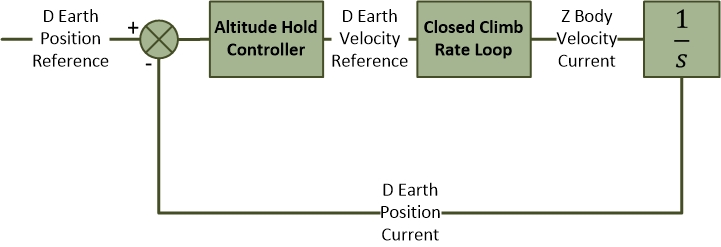
\includegraphics[height = 4cm]{../References/Diagrams/AltHoldLoop.jpg}
	 	\caption{Altitude Hold Controller Closed Loop}
	 	\label{IM_AltHoldControlLoop}
	 \end{figure}
	 
	 The chosen controller architecture is shown in Figure \ref{IM_AltHoldController}. The proportional gain is used to vary the bandwidth to be within the limits of the system. An limited integrator is added to reject measurement errors in the inner loops, this component is represented by the faded integrator shown in Figure \ref{IM_AltHoldController} is not considered during linear analysis. The integrator shall be limited in such a way as to limit the interference of the proportional gain. This approach reduces the maximum disturbance rejection this controller can handle. To increase the bandwidth of the disturbance rejection capabilities, a PID controller architecture was also considered and the analysis was done for both control laws.
	 
	 The system's dynamic response is analysed using the root locus shown in Figure \ref{IM_AltHoldRoot} and the bode plot shown in Figure \ref{IM_AltHoldBode}.
	 
	 \begin{figure}[H]
	 	\centering
	 	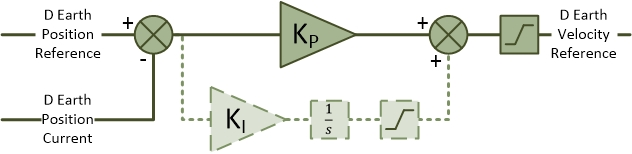
\includegraphics[height = 3.5cm]{../References/Diagrams/AltHoldController.jpg}
	 	\caption{Altitude Hold Controller}
	 	\label{IM_AltHoldController}
	 \end{figure}
	 
	 Figures \ref{IM_AltHoldRoot} and \ref{IM_AltHoldBode} evaluate a P controller against a PID controller. The dominant closed loop poles of the P controlled system are placed at $-2.03 \pm 0.58i$ and are slightly under damped with a damping ratio of $0.96$. 

	 The PID controller adds an additional pole and two additional zeros into the system. The closed loop poles of the PID controlled system are located at $-6.64$, $-3.59 \pm 5.03i$ and $-0.64 \pm 0.47i$. The two new zeros are placed at $-0.57$ and $-2.06$.
	 
	 \begin{figure}[H]
	 	\centering
	 	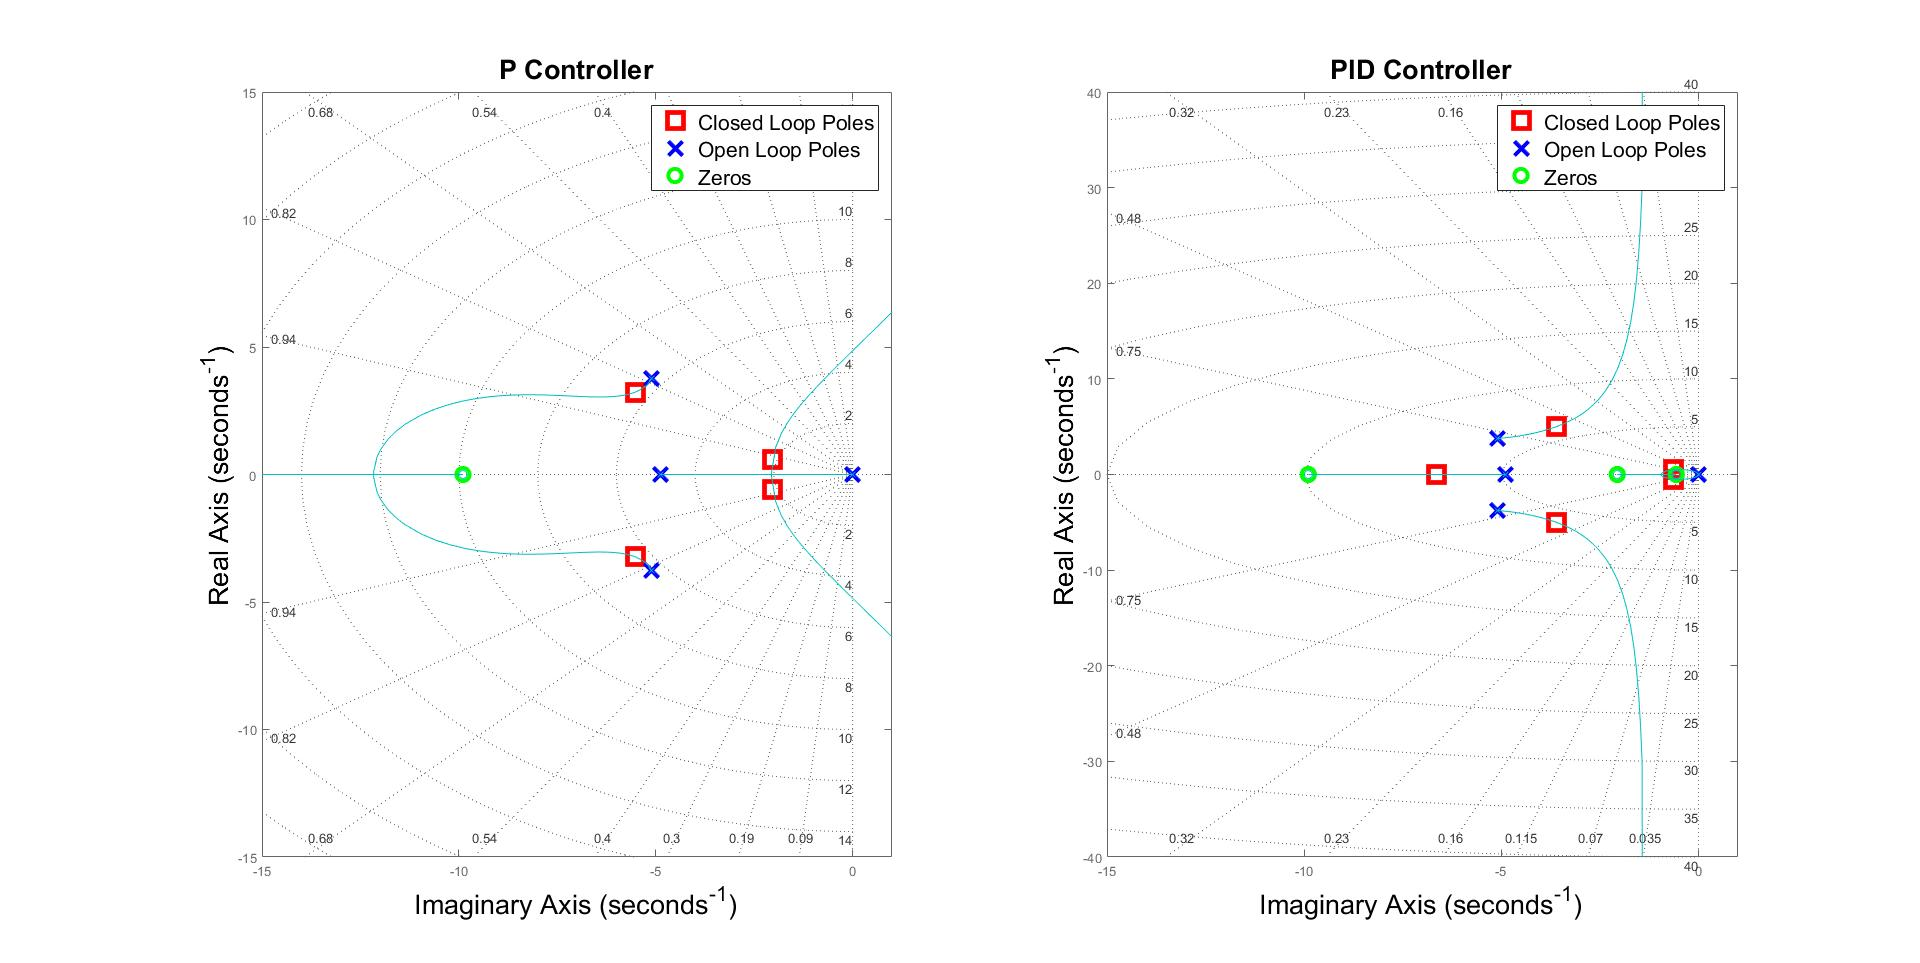
\includegraphics[height = 7.9cm]{../Design/Matlab/Controllers/altitude_root.jpg}
	 	\caption{Altitude Hold Controller -  Root Locus}
	 	\label{IM_AltHoldRoot}
	 \end{figure}
	 
	 The bode plot shows the PID controller producing a final cross over frequency of $1.90Rad/s$, this response is too fast for the inner climb rate system and will need to be redesigned or discarded. The P controller exhibits a cross over frequency of $0.91Rad/s$, this produces a ratio of $3.03$ between the inner and outer loops and a phase margin of $71.5$\textdegree. The phase of the system using a P controller crosses the $180$\textdegree  $\ $mark at $4.81Rad/s$ and has a gain margin of $18.7dB$.
	 
	 \begin{figure}[H]
	 	\centering
	 	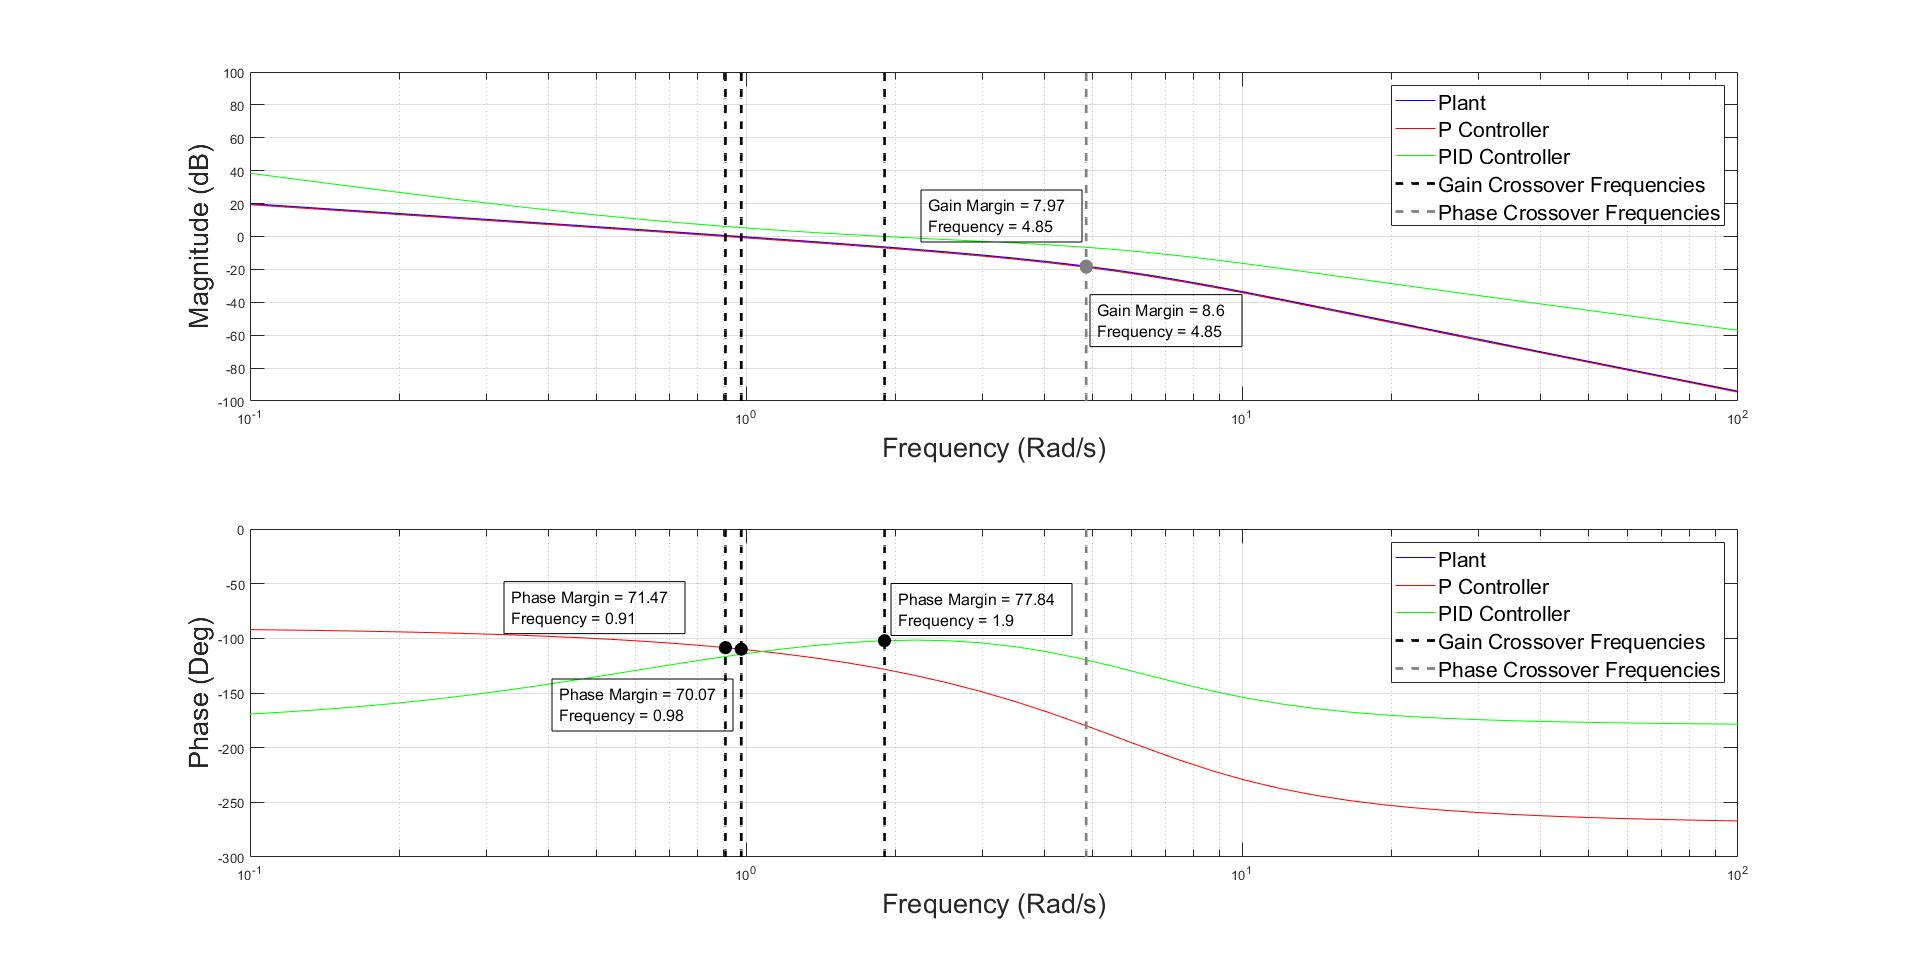
\includegraphics[height = 7.9cm]{../Design/Matlab/Controllers/altitude_bode.jpg}
	 	\caption{Altitude Hold Controller -  Bode Plots}
	 	\label{IM_AltHoldBode}
	 \end{figure}
	 
	 To finalise the design, the two limiters are discussed. The first limiter is used to limit the effect of the integrator on the system as well as stop integrator wind up. The second limiter is used to limit the climb rate commands sent to the inner controllers. Both sets of limits are shown in Table \ref{tab:AltitudeControllerLimits}
	 
	 \begin{table}[!]
	 	\centering
	 	\begin{tabular}{l | c | c |}
	 		Limit Name 						& Min & Max\\
	 		\hline\hline
	 		Integrator Wind Up 				& -0.09 & 0.09 \\
	 		Climb Rate Command 		    	& -5 & 5 \\
	 	\end{tabular}
	 	\caption{Altitude Hold Controller Limits}
	 	\label{tab:AltitudeControllerLimits}
	 \end{table}
	 
		 \subsubsection{Altitude Hold Controller Discussion}
		 Although both the P and PID controllers exhibit stable dynamic responses, the PID controller exhibited too fast a response and will be influenced by the inner controllers. The system including only a P controller exhibits a step response as shown in Figure \ref{IM_AltHoldStep}, a disturbance of $10N$ is applied to the rotors at $10s$. The system has a $5\%$ settling time of $2.29s$ and tracks the set point with zero steady state error. The system handles the disturbance with a maximum overshoot of $0.01m$ and is critically damped.
		 
		 \begin{figure}[H]
		 	\centering
		 	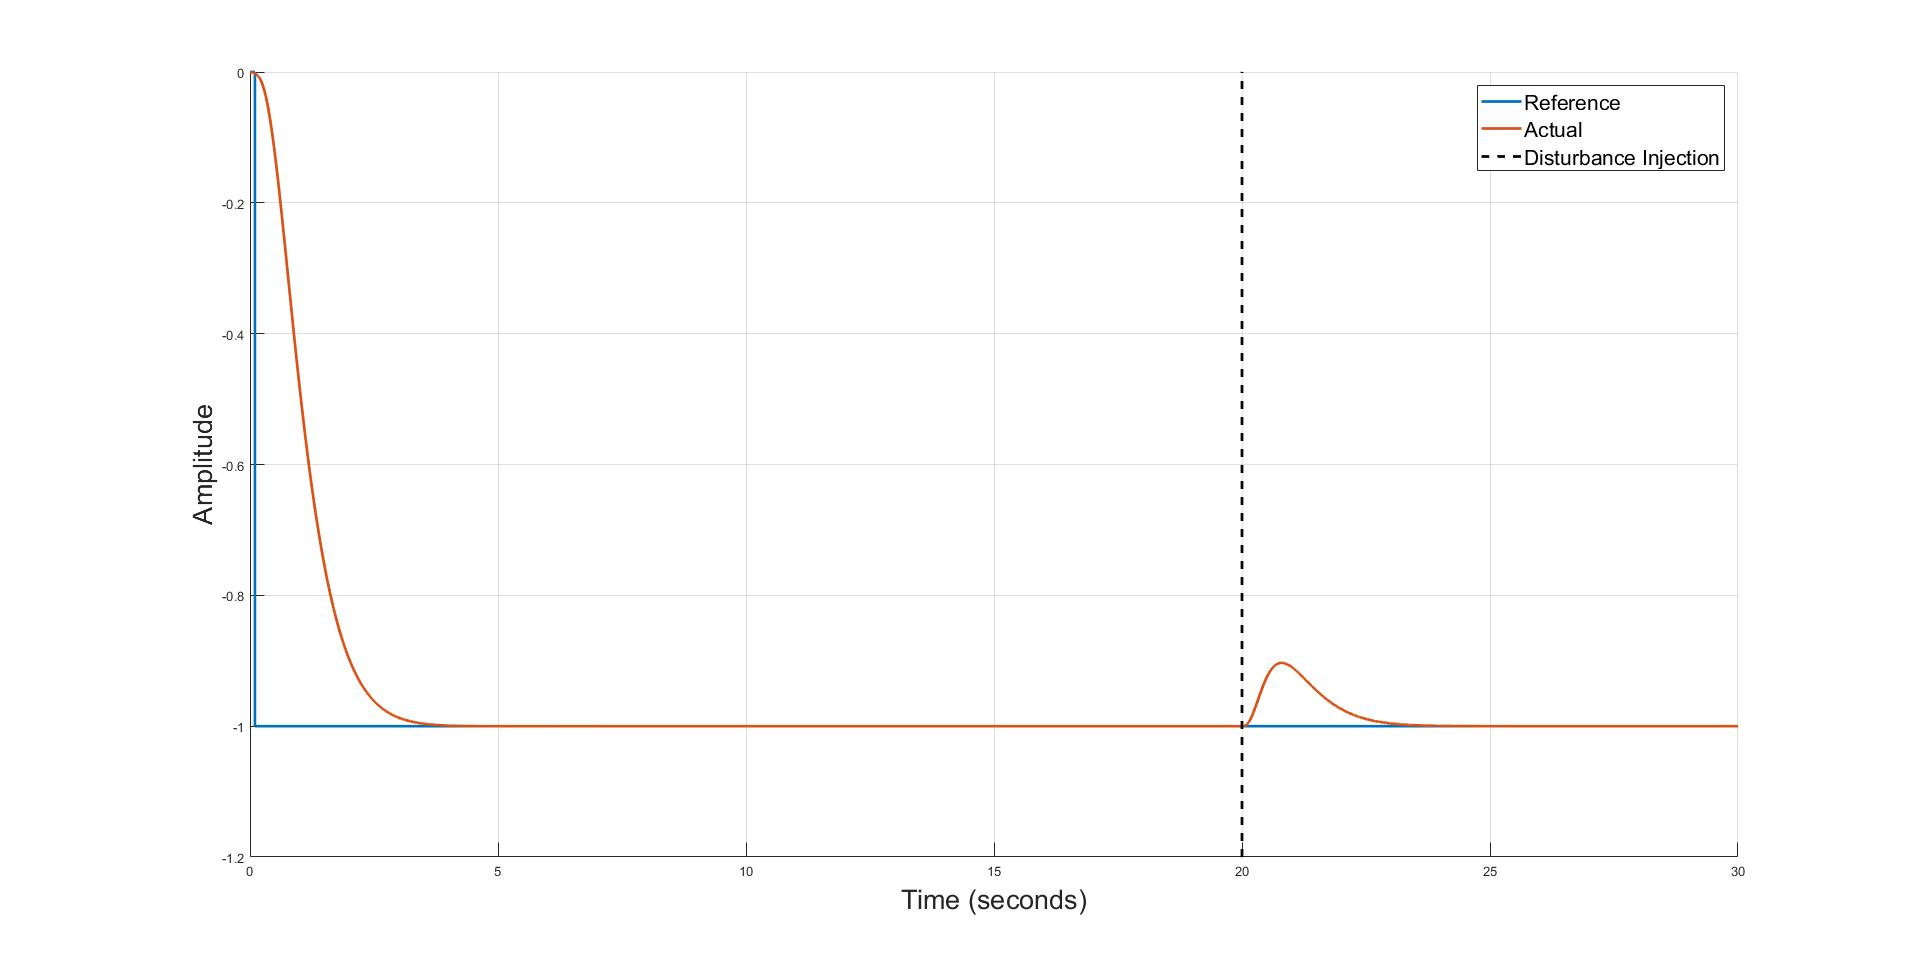
\includegraphics[height = 8cm]{../Design/Matlab/Controllers/altitude_step_p_no_dist.jpg}
		 	\caption{Altitude Hold P Controller -  Step response}
		 	\label{IM_AltHoldStep}
		 \end{figure}
		 
		 However, if a measurement disturbance is present in the inner loops, this system will not track a setpoint with zero steady state error. To demonstrate this a constant offset of $0.05m/s$ is placed on the Z-Axis velocity measurement, Figure \ref{IM_AltHoldPDistStep} shows the current system cannot account for this disturbance. As shown in \ref{IM_AltHoldController}, a limited gain integrator is introduced into the system to help the system track steady state error. 
		 
		 \begin{figure}[H]
		 	\centering
		 	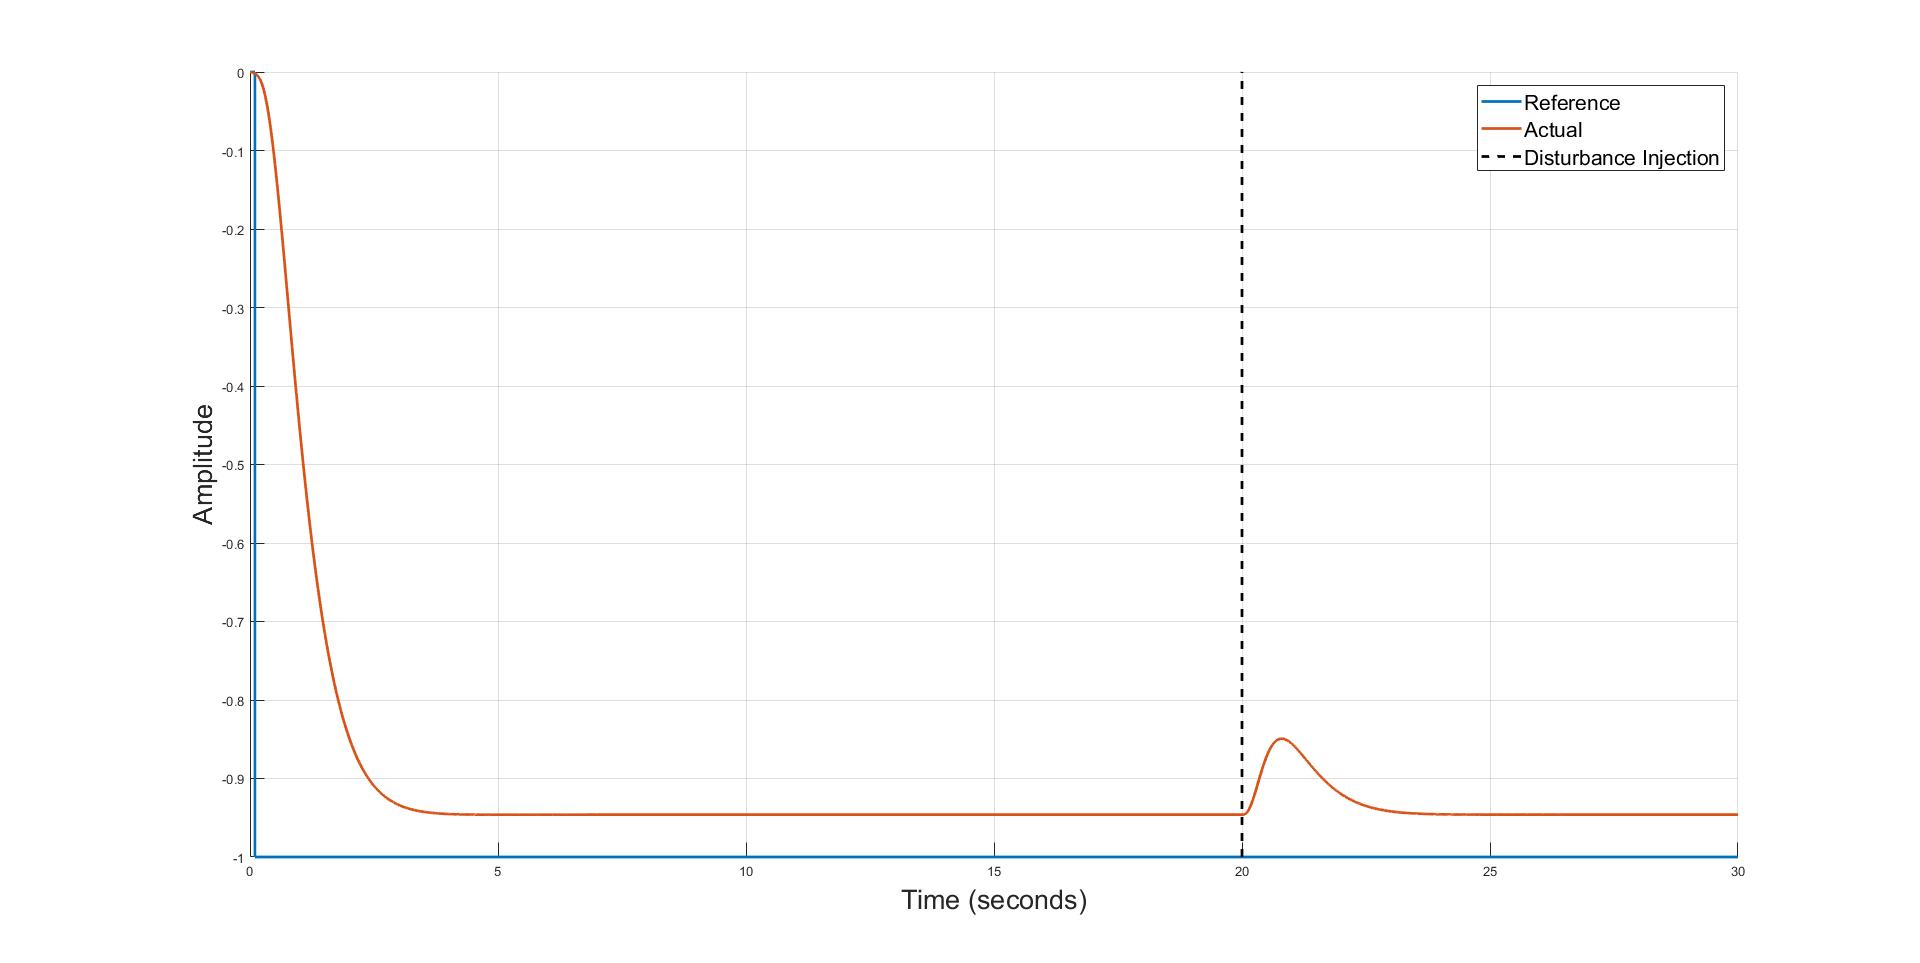
\includegraphics[height = 8cm]{../Design/Matlab/Controllers/altitude_step_p_dist.jpg}
		 	\caption{Altitude Hold P Controller -  Step response with inner loop measurement offset}
		 	\label{IM_AltHoldPDistStep}
		 \end{figure}
		 
		 The new controller must be limited in such a way as to exhibit a similar transient response as the existing P controller. Figure \ref{IM_AltHoldPIDistStep} shows the step response of the new system both with and without the $0.05m/s$ offset in the velocity measurement. As shown, the P controller including a limited I component introduces more overshoot into the system. The limits are designed to ensure the new controller introduces less than 10\% overshoot into the system. 
		 
		 \begin{figure}[H]
		 	\centering
		 	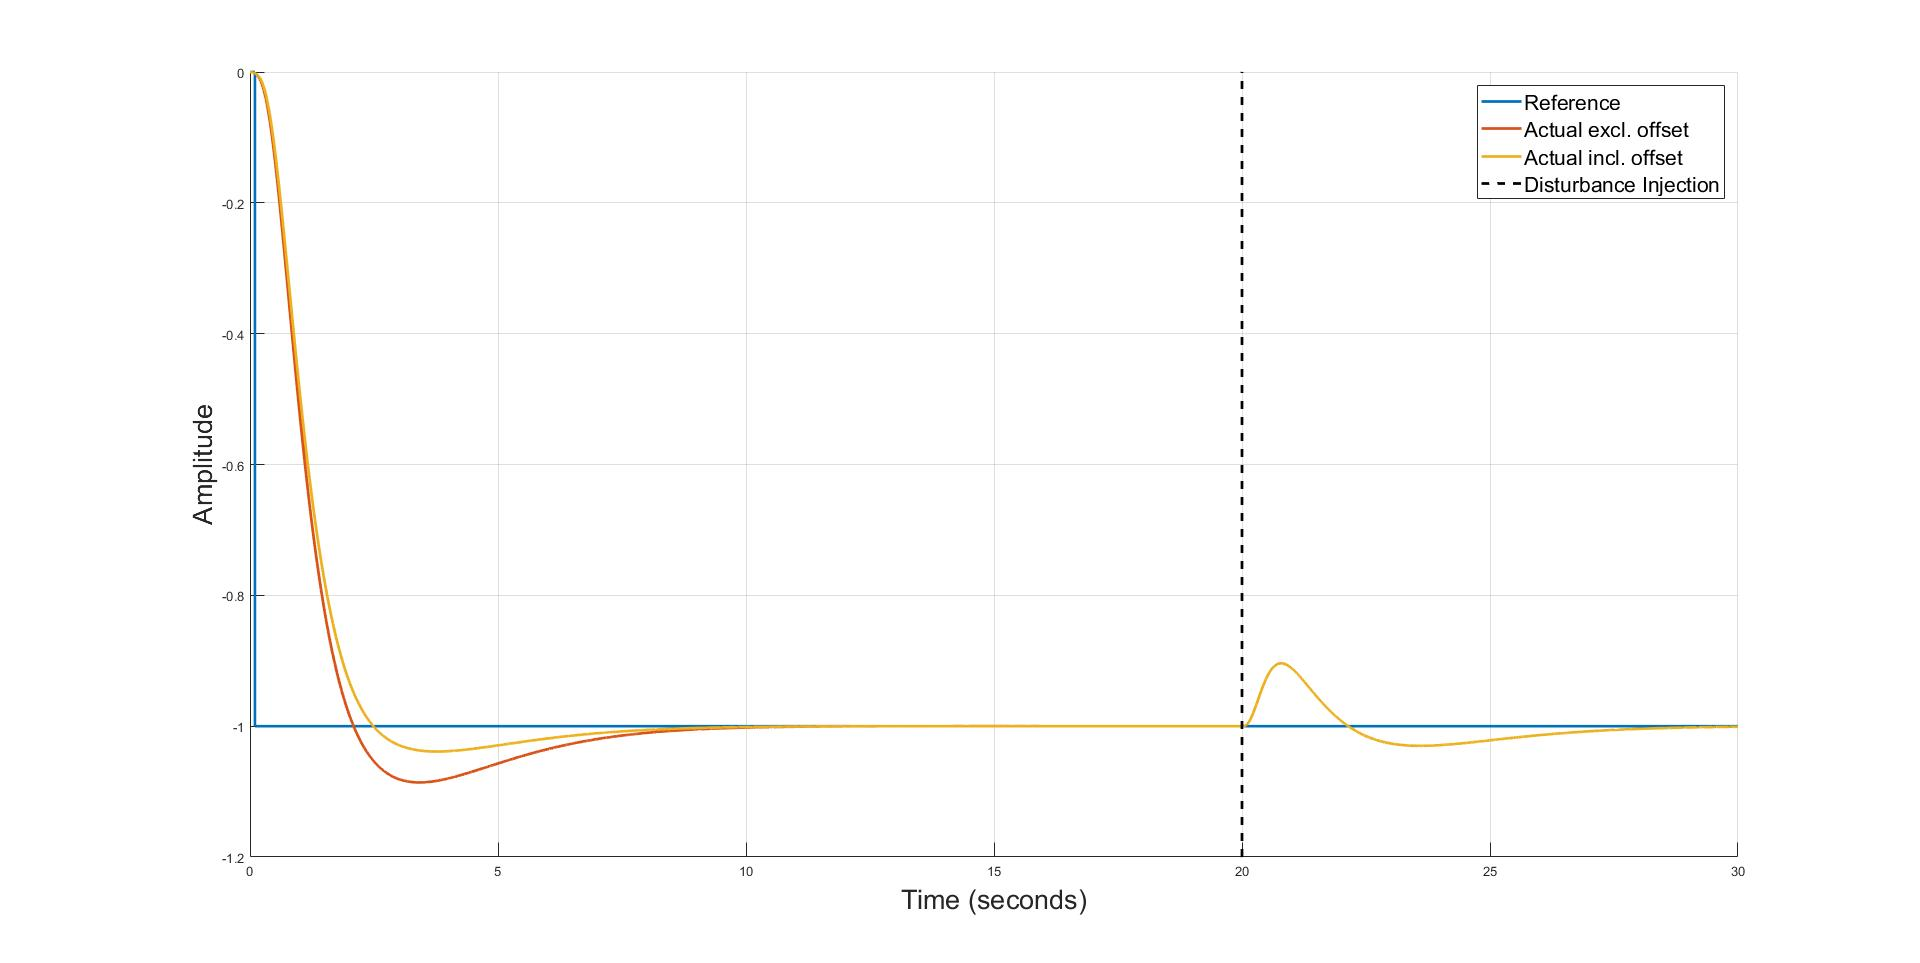
\includegraphics[height = 8cm]{../Design/Matlab/Controllers/altitude_step_pi.jpg}
		 	\caption{Altitude Hold P with Limited I Controller -  Step Responses}
		 	\label{IM_AltHoldPIDistStep}
		 \end{figure}
	 
\section{Horizontal Control}
This section describes the horizontal controller. This system is responsible for controlling the craft's North and East position in the earth frame, to do this the controller's most inner loop commands the pitch and roll rates of the craft. The narrow, confined spaces in which the craft must fly means it is very important for the horizontal controller to respond quickly to commands and disturbances. The limited space also limits the amount of allowed overshoot, requiring a well damped final system. The system must ensure it stay within the thrust limits as to not affect the other controllers. The controller will need to be able reject disturbances caused by wind, sensor offsets and unbalanced rotors. To handles these disturbances and other, the system will require an integrator in the controller. The integrator should be fast enough as to ensure the system stays within it's narrow, permissible flight region, even during disturbances.

The horizontal controller is designed as two sets of four cascaded control loops, one set for roll and one set for pitch. The most inner loop controls either the roll or pitch rate of the craft by commanding the virtual actuators $\delta_\phi$ and $\delta_\theta$ respectively. The desired angular rates are in turn commanded by the tilt angle controller. The tilt angle controller is responsible for converting desired translational accelerations into desired roll and pitch angles. These acceleration setpoints are commanded by the linear velocity controller which receives it's setpoint from the most outer global position controller. The global position controller will receive it's setpoint from the waypoint generation method described in a proceeding section. This section begins by deriving the plant dynamics for roll and pitch.
	
	\subsection{Roll and Pitch Rate Dynamics}
	The roll and pitch acceleration dynamics can be derived using Newton mechanics at near hover conditions and the craft's inertia around the X-axis ($I_{xx}$) and the Y-axis ($I_{yy}$) respectively, the result is shown in \eqref{EQ_RollNewton} and \eqref{EQ_PitchNewton}.
	
	\begin{equation}
	\label{EQ_RollNewton}
	\dot{p} = \dfrac{L}{I_{xx}}
	\end{equation}
	
	\begin{equation}
	\label{EQ_PitchNewton}
	\dot{q} = \dfrac{M}{I_{yy}}
	\end{equation}
	
	The rotors introduce an additional timing delay into the dynamics, as shown in \eqref{EQ_MotorDelay}. The state space equation for both systems can be derived using the current angular rates ($p$ \& $q$) and the current angular moments ($L$ \& $M$) as the system states. The state space representation for roll is shown in \eqref{EQ_RollStateSpace1} and \eqref{EQ_RollStateSpace2}. The transfer function for roll acceleration can subsequently be calculated from the state space representation. Integrating the result produces the transfer function for roll rate as shown in \eqref{EQ_RollTF}. The same approach is followed for deriving the pitch rate dynamics shown in \ref{EQ_PitchTF}.
	
	\begin{eqnarray}
	\begin{bmatrix} \dot{L} \\ \dot{p}	\end{bmatrix}&=&\begin{bmatrix}\frac{1}{\tau}\ \ \ \ \ 0\\\frac{1}{I_{xx}} \ \ \ 0 \end{bmatrix} \begin{bmatrix} L \\ p \end{bmatrix} + \begin{bmatrix}\frac{1}{\tau}\\ 0 \end{bmatrix} \delta_\phi\label{EQ_RollStateSpace1}\\\label{EQ_RollStateSpace11} 
	y &=& \begin{bmatrix} 0 \ \ \ \ 1 \end{bmatrix} \begin{bmatrix} L \\ p \end{bmatrix} \label{EQ_RollStateSpace2}\\
	G(s)_{roll} &=& \frac{\frac{1}{\tau I_{xx}}}{s (s + \frac{1}{\tau})}\label{EQ_RollTF}\\
	G(s)_{pitch} &=& \frac{\frac{1}{\tau I_{yy}}}{s (s + \frac{1}{\tau})}\label{EQ_PitchTF}
	\end{eqnarray}
	
	The roll and pitch plants both have a naturally occurring integrator, an open loop pole at $-\dfrac{1}{\tau}$ and no naturally occurring zeros. As shown, the plant gain is inversely proportional to the specific axis inertia. The design of the craft creates a smaller pitching plant gain than rolling plant gain. The design however, gives the pitching moment a longer torque arm, creating a larger actuation torque.
	
	\subsection{Roll and Pitch Rate Controllers}
	The roll and pitch rate controllers are the most inner loops of the horizontal controller and they command the $\delta_\phi$ and $\delta_\theta$ virtual actuators respectively. As the most inner controllers the outer loops of the horizontal controller are limited by the response and bandwidth of this system. Both these systems should then utilise as much bandwidth as the physical motor-rotor system allows. Section \ref{SSECT_Disturbances} describes some of the expected disturbances where induced moments can be caused in multiple scenarios. Including being in near proximity with a wall or having unbalanced rotor pairs. The final system must track a set point with zero steady state error. To meet the horizontal controller's requirement of fast disturbance rejection, the roll and pitch rate controllers, as the fastest controllers, should include an integrator. 
	
	The integrator will slow the system down, which can be subsequently sped up with a lead compensator. However, the final commanded motor thrusts must be validated against the limits provided in Table \ref{tab:HeadRoomPercentages}. The final controller architecture is shown in Figure \ref{IM_RollPitchRateController}. The controller gain values must be chosen such that the inner rate system is robust to unmodelled errors and have a sufficient gain and phase margin.
	
	\begin{figure}[H]
		\centering
		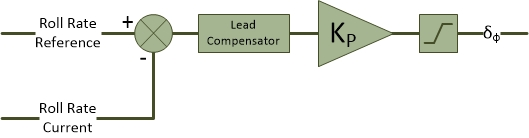
\includegraphics[height = 3.3cm]{../References/Diagrams/RollRateController.jpg}
		\caption{Roll and Pitch Rate Controller Design}
		\label{IM_RollPitchRateController}
	\end{figure}	
		
	First, the dynamic response of the controlled roll system is evaluated using the root locus shown in Figure \ref{IM_RollRateControlRoot}. To maintain good damping, the two dominant poles are kept close to the imaginary axis and have a final damping ratio of $0.9$. Where the placement of the slower zero dictates how much influence the integrator can have on the system.
	
	\begin{figure}[H]
		\centering
		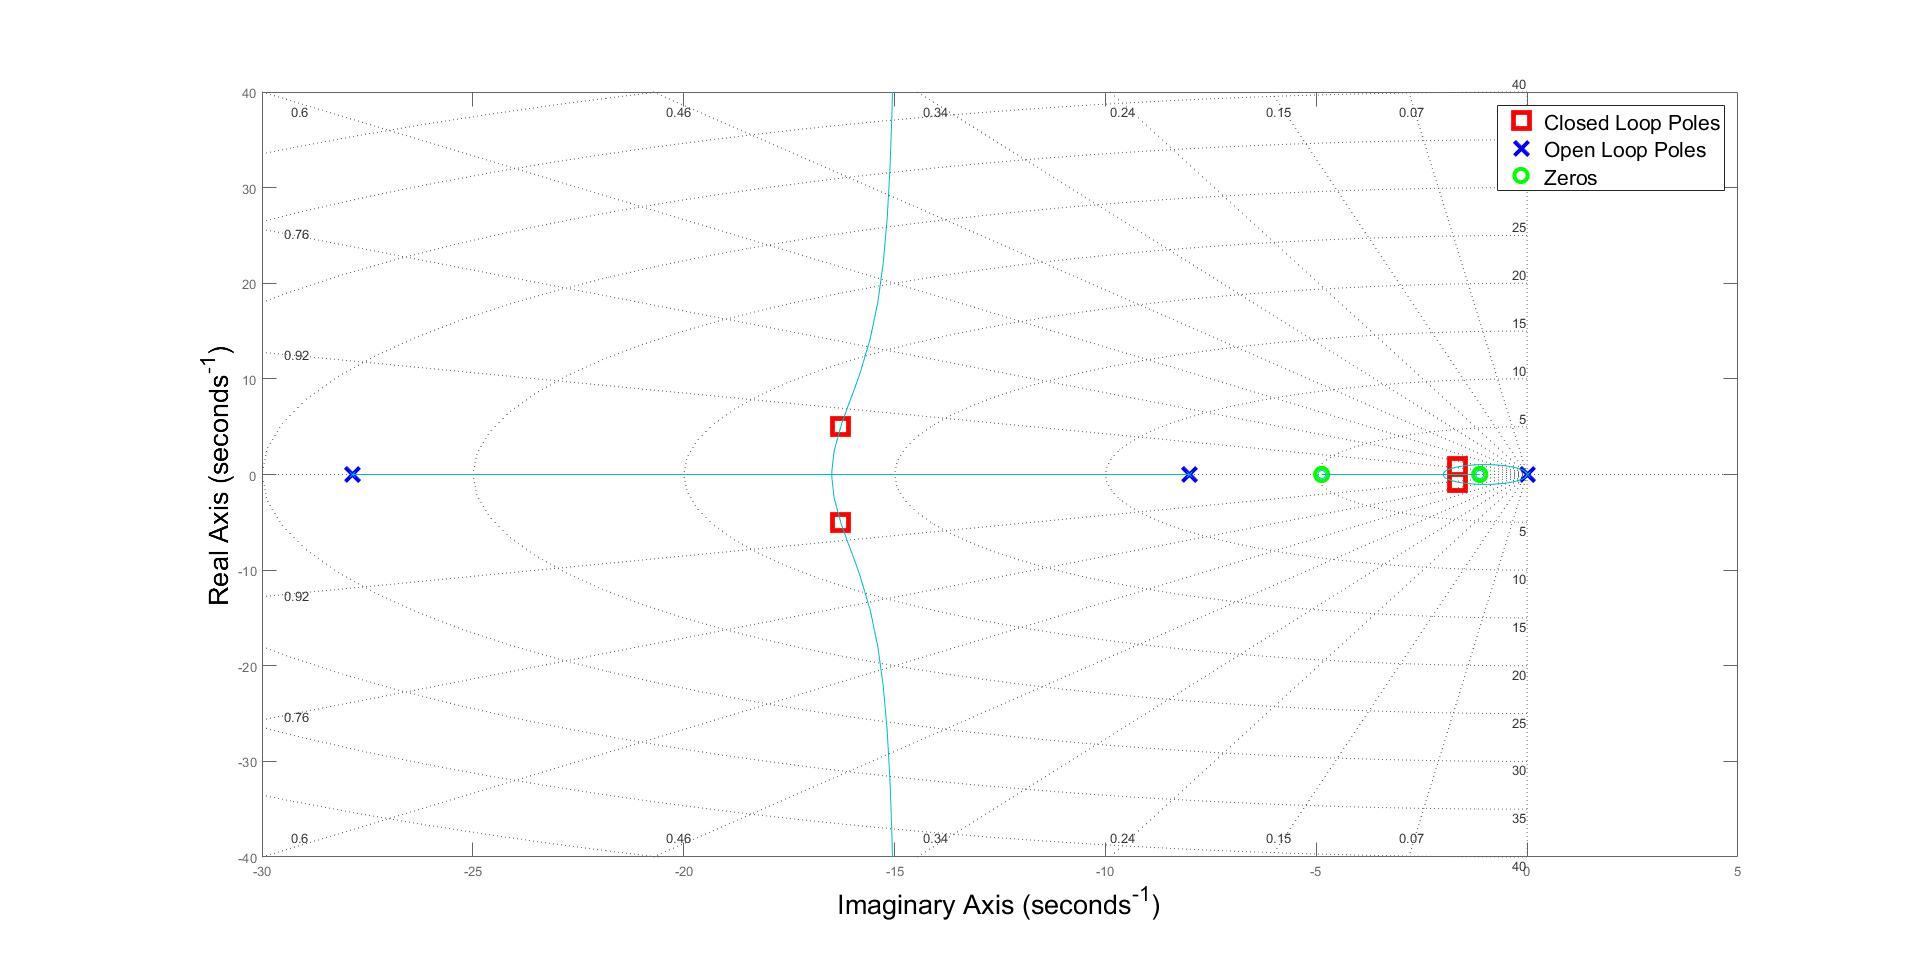
\includegraphics[height = 8cm]{../Design/Matlab/Controllers/roll_rate_root.jpg}
		\caption{Roll Rate Controller -  Root Locus}
		\label{IM_RollRateControlRoot}
	\end{figure}
	
	The frequency response of the roll system is then investigated using the Bode plot shown in Figure \ref{IM_RollRateControlBode}. Unity feedback is compared against the chosen controller. The high natural gain of the rolling system gives unity feedback a very fast result with too much bandwidth for the physical system to match. There is also an insufficient phase margin of $25$\textdegree\,in the system and no offset disturbance rejection. The controller adds an integrator to reject disturbances, this however reduces phase even more and slows the system. The lead compensator is then used to increase the phase and bandwidth and reach a final phase margin of $80.6$\textdegree\,with a crossover frequency of $4.75$\,rad/s.
	
	\begin{figure}[H]
		\centering
		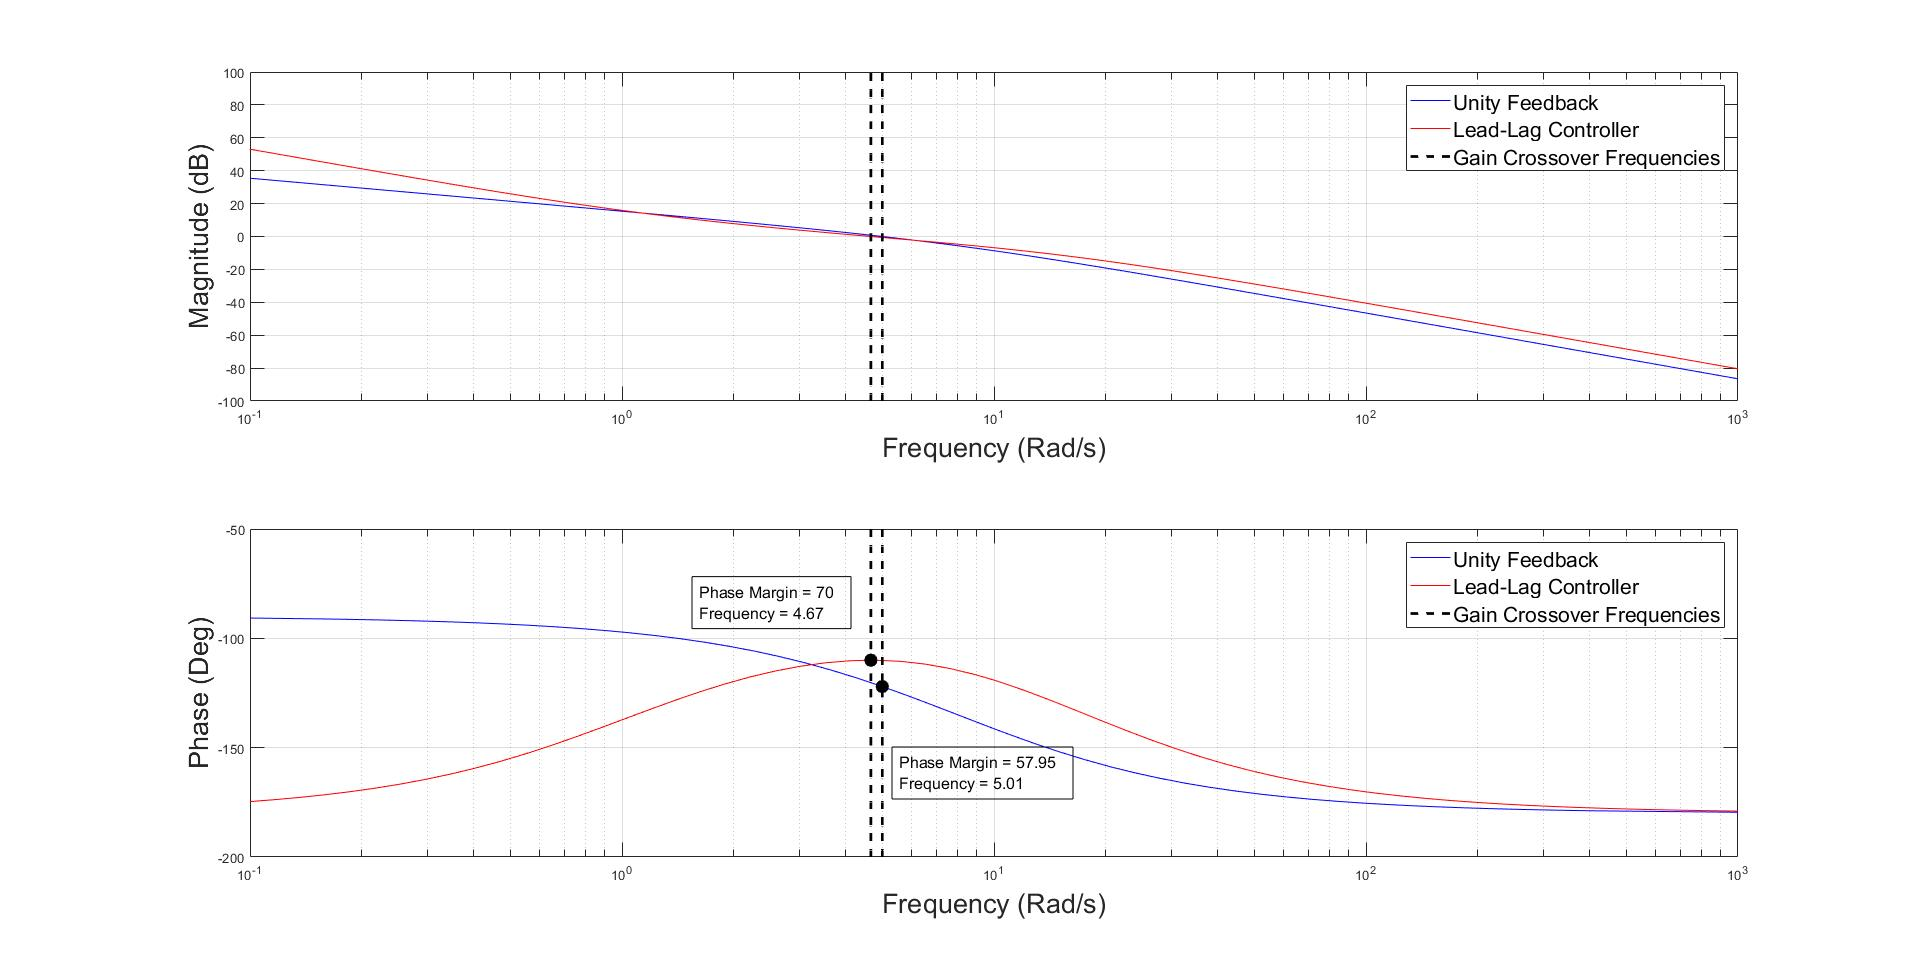
\includegraphics[height = 8cm]{../Design/Matlab/Controllers/roll_rate_bode.jpg}
		\caption{Roll Rate Controller -  Bode Plot}
		\label{IM_RollRateControlBode}
	\end{figure}
	
	Next the pitch rate system is evaluated. The loci and closed loop poles of the controlled pitch system can be shown to be similar to the roll system. However, the pitching plant is naturally slower and has less gain than the rolling system. The pitch rate controller is thus required to have more gain than the roll rate controller. The Bode plot shown in Figure \ref{IM_PitchRateControlBode} is used to evaluate the frequency response of the pitch rate system. Unity feedback is compared against the implemented Lead-Lag controller. As shown the natural system with unity feedback produces a much lower crossover bandwidth than the natural roll system. As with the roll rate controller, the integrator included in the controller reduces phase and bandwidth in the system but also enables disturbance rejection. To speed up the system, a similarly placed lead compensator is used. This increases the phase and bandwidth to reach a final phase margin of $82.2$\textdegree\,with a crossover frequency of $4.72$\,rad/s.
	
	\begin{figure}[H]
		\centering
		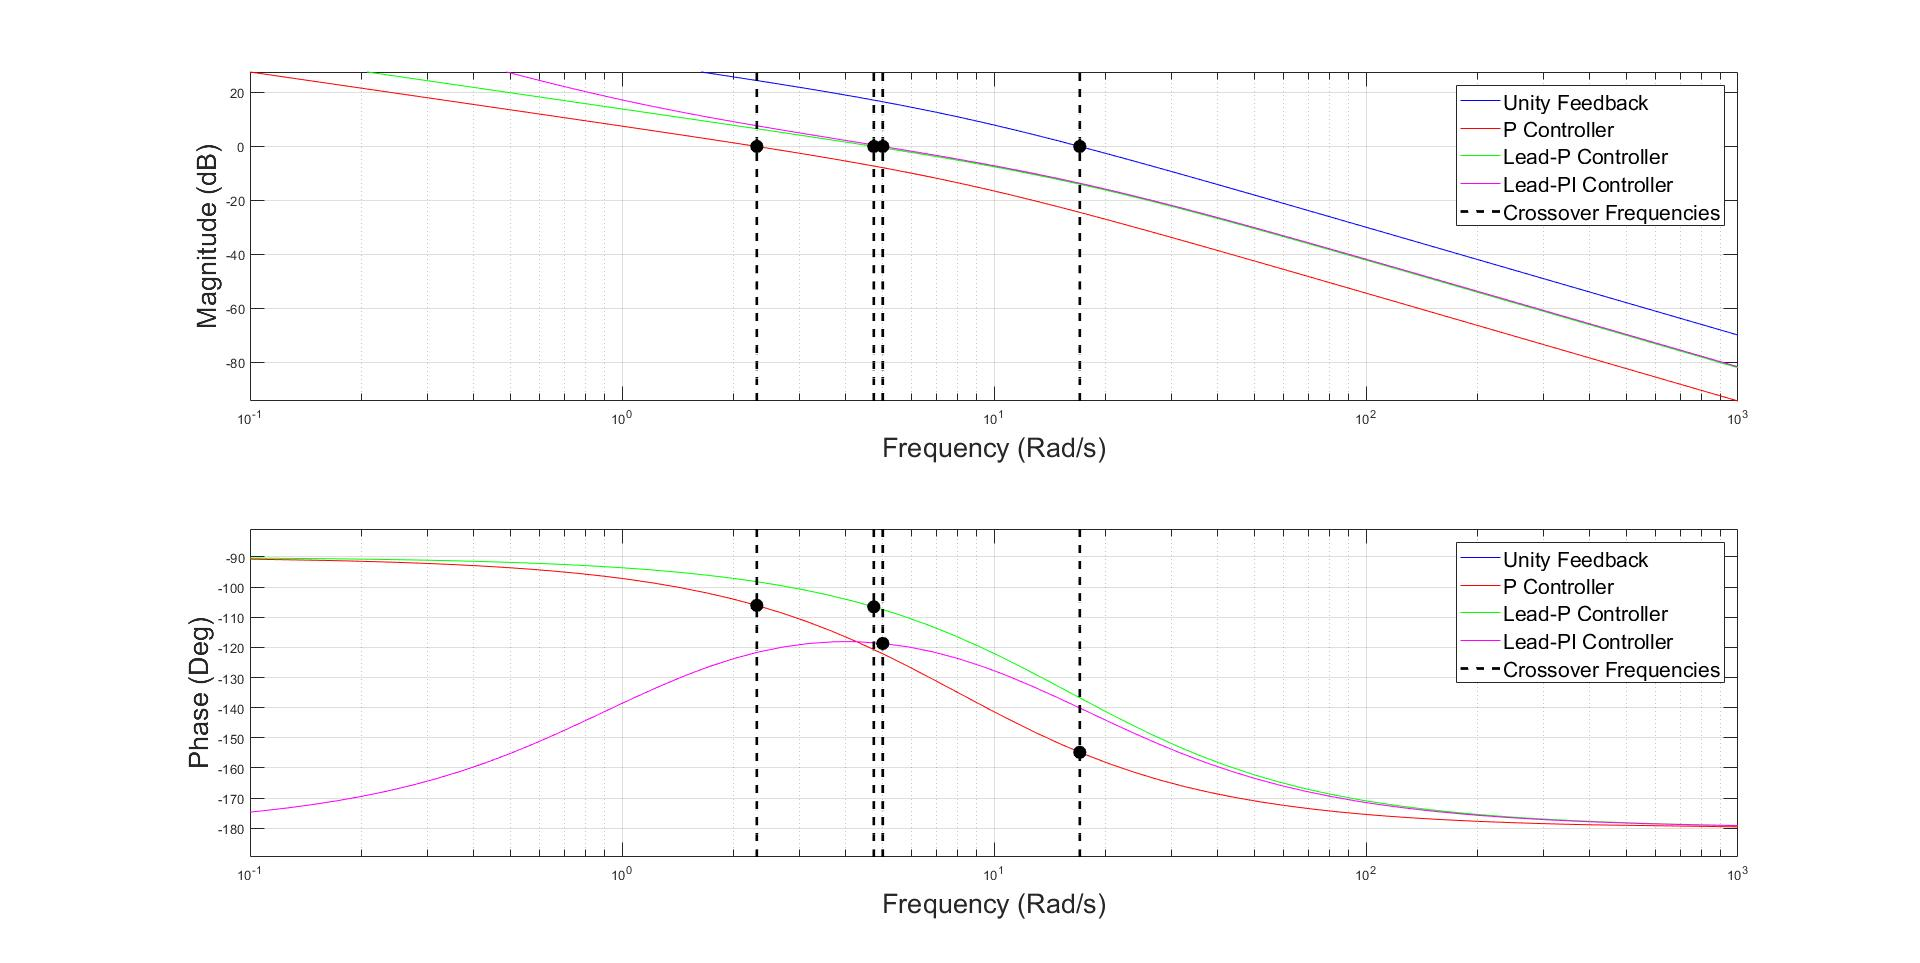
\includegraphics[height = 8cm]{../Design/Matlab/Controllers/pitch_rate_bode.jpg}
		\caption{Pitch Rate Controller -  Bode Plot}
		\label{IM_PitchRateControlBode}
	\end{figure}
		
		
		\subsubsection{Roll and Pitch Rate Controller Discussion}
		The dynamic responses of the roll and pitch rate systems is shown to be robust, damped and they both utilise the full bandwidth allowed by the system characteristics. The integrator term in both controllers will ensure that the rate loop can handle steady state disturbances. To stop integrator wind up however, the controllers include a saturation on the integral term. Although both systems have the same controller architecture, the physical design of the craft means the roll system will have a larger plant gain. It is desired that the roll and pitch rate systems have similar closed loop responses which means the pitch rate controller needs to have increased gain compared to the roll rate controller. This unfortunately leaves the roll rate controller to be more susceptible to disturbances. The flight strategy should take this into consideration and negate rolling disturbances as much as possible.
		
		This characteristic can be shown in the time domain using step responses and the maximum impulse required of the motors. To enable a comparison between the systems, the step response of both the roll and pitch rate system is shown in Figure \ref{IM_PitchRateStep}. To simulate a disturbance, a $0.05$\,Nm loss in torque is applied to the roll system at $5$\,s. The pitching system experiences a disturbance of $0.2$\,Nm. Both disturbances are calculated and equivalent to two rotors, on the same side, instantaneously losing $0.25$\,N of thrust.
		
		\begin{figure}[H]
			\centering
			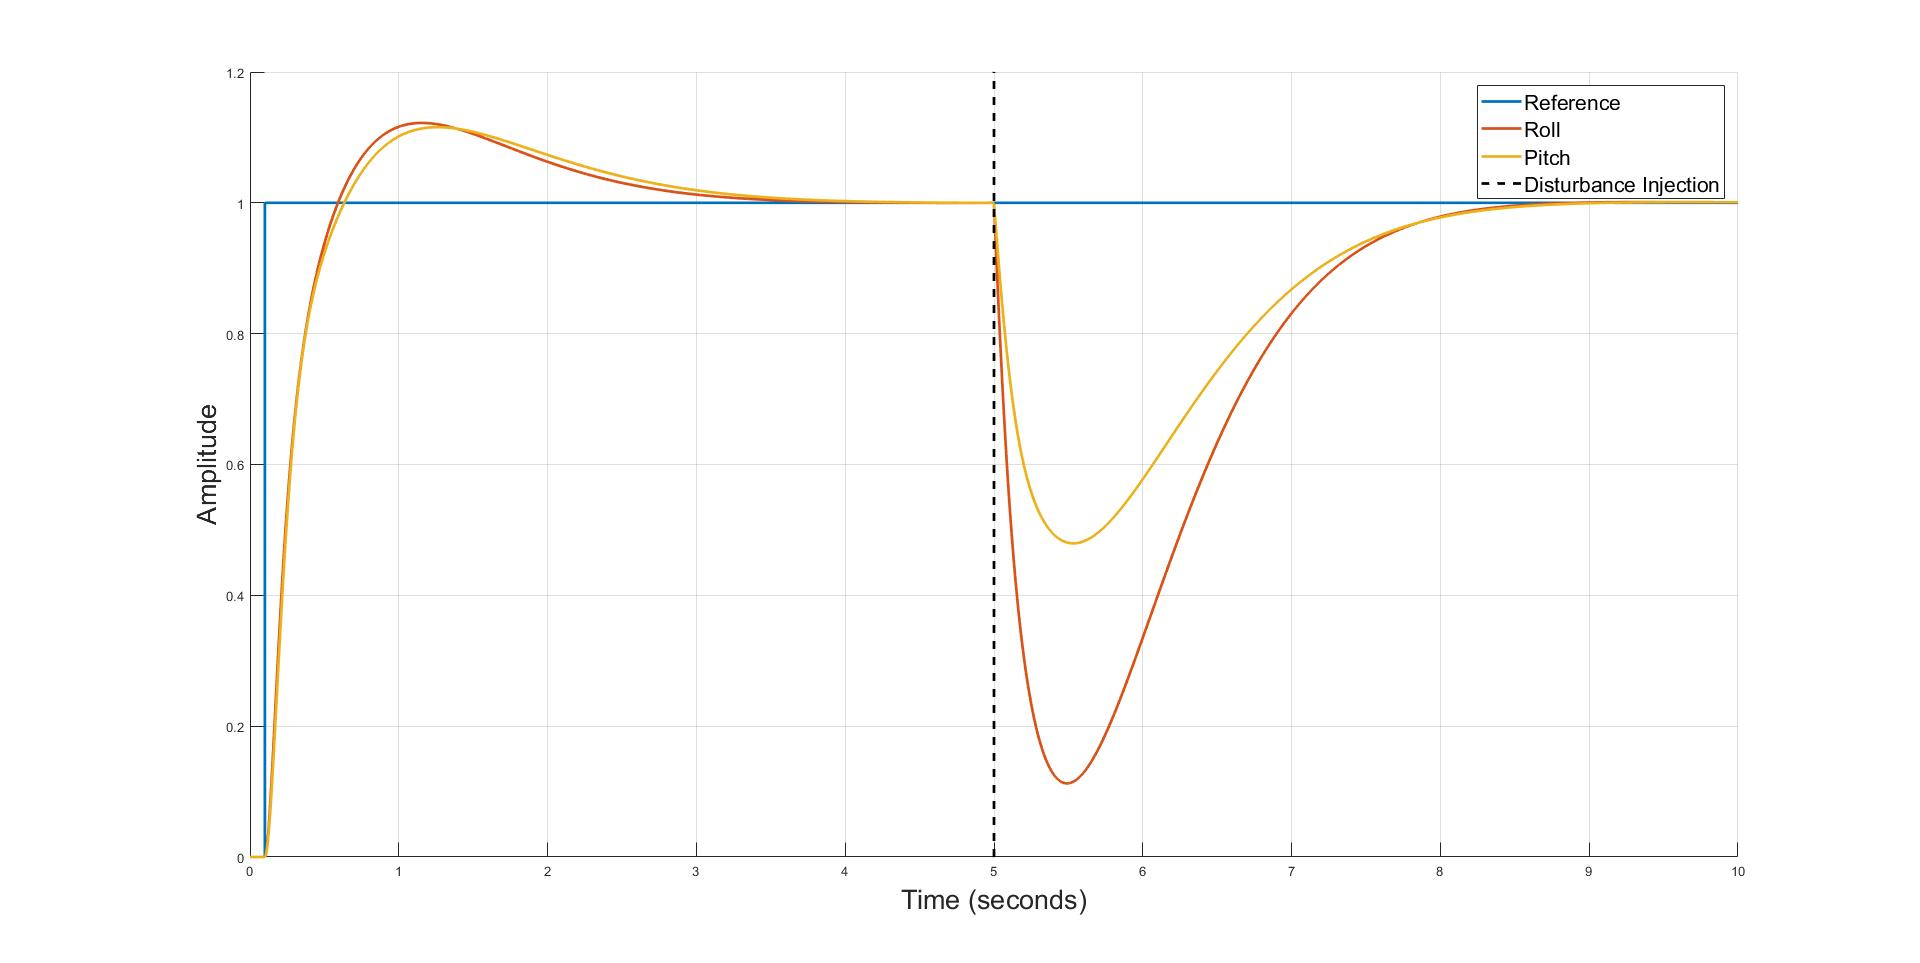
\includegraphics[height = 8cm]{../Design/Matlab/Controllers/roll_pitch_rate_step.jpg}
			\caption{Pitch Rate Controller -  Step Responses}
			\label{IM_PitchRateStep}
		\end{figure}
		
		Both the roll and pitch closed loop systems have similar transient responses. The pitch rise time of $0.33$\,s is very similar to the roll rise time of $0.32$\,s. The pitch $5$\,\% settling time is measured at $2.2$\,s which is also very close to the rolling settling time of $2.1$\,s. Both systems are similarly damped and have overshoot of $12$\,\%. Limiting the integral term can reduce the overshoot however, this will also limit the disturbance rejection capabilities of the system. Both the roll and pitch systems handle the disturbance successfully and settle back within $5$\,\% of the setpoint in $2.6$\,s. As expected, the roll system has more difficulty handling the disturbance.

		The commands sent to the rotors during the roll step are shown in Figure \ref{IM_RollRateImpulse} with a maximum commanded thrust of $0.49$\,N. Similarly, the pitching motor outputs are shown, in Figure \ref{IM_PitchRateImpulse}, to have a maximum thrust of $0.69$\,N.
		
		\begin{figure}[H]
			\centering
			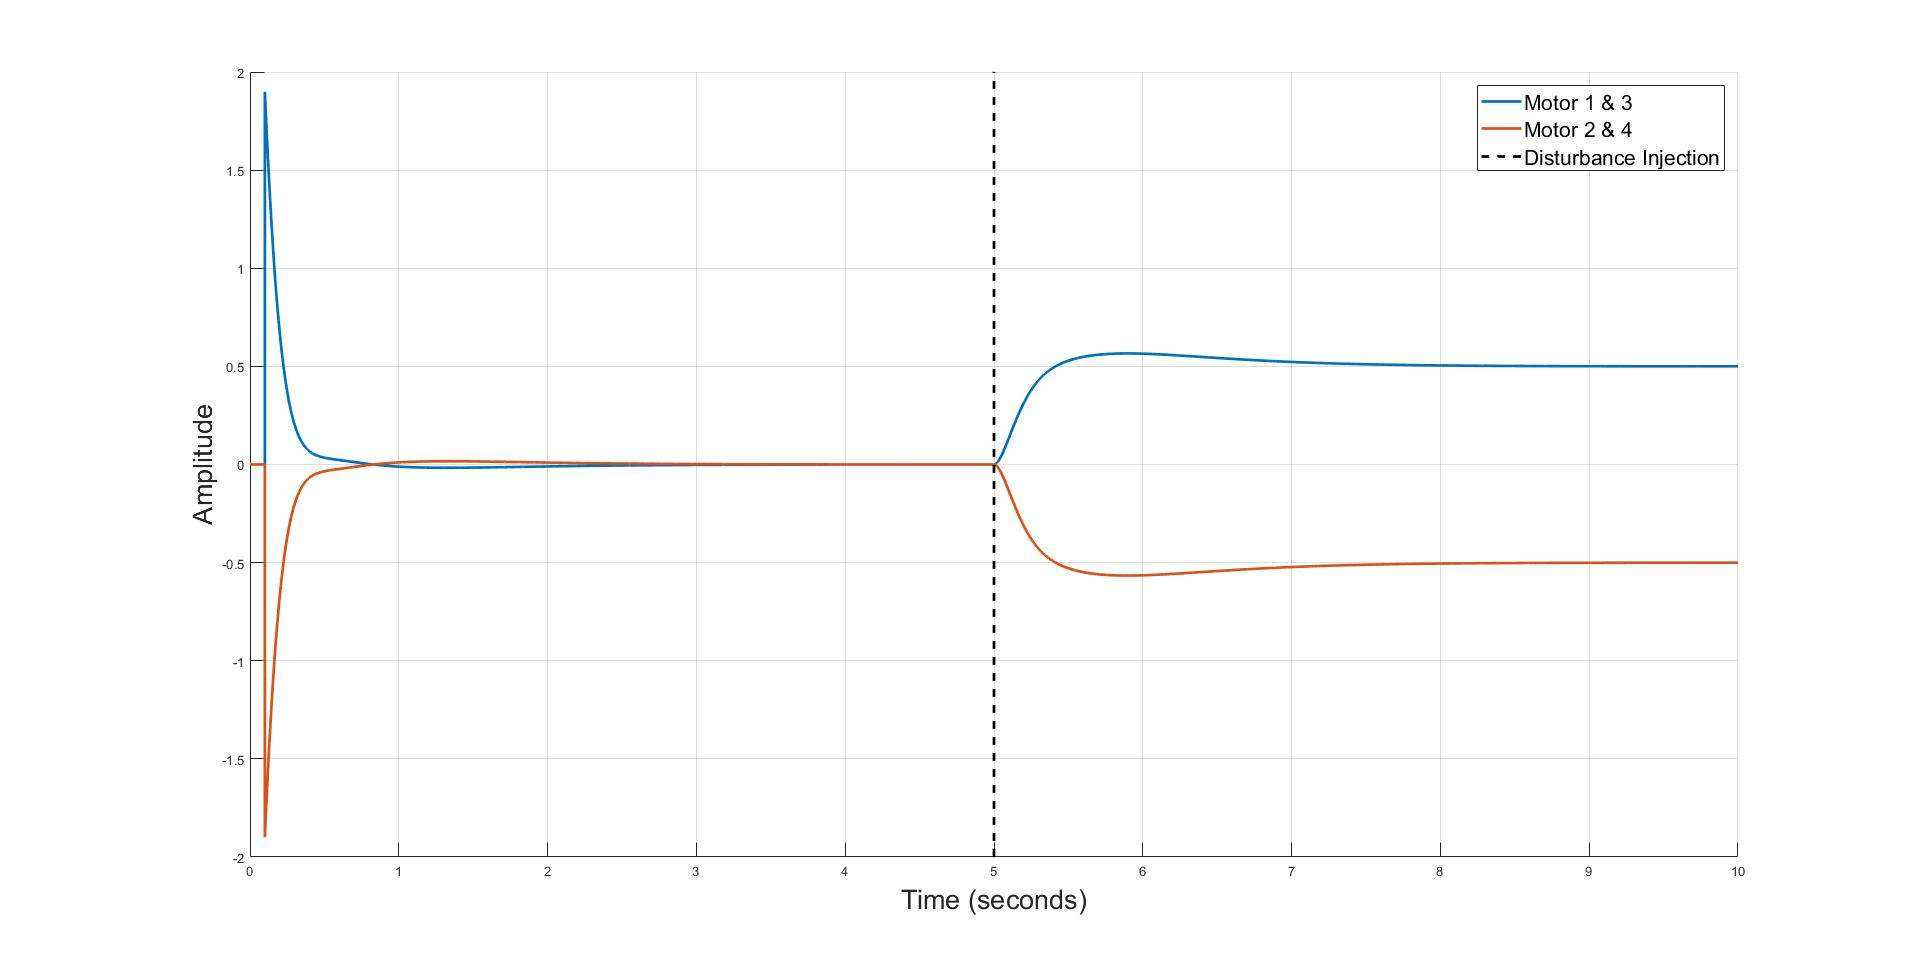
\includegraphics[height = 8cm]{../Design/Matlab/Controllers/roll_rate_impulse.jpg}
			\caption{Roll Rate Controller -  Motor Commands}
			\label{IM_RollRateImpulse}
		\end{figure}
		
		\begin{figure}[H]
			\centering
			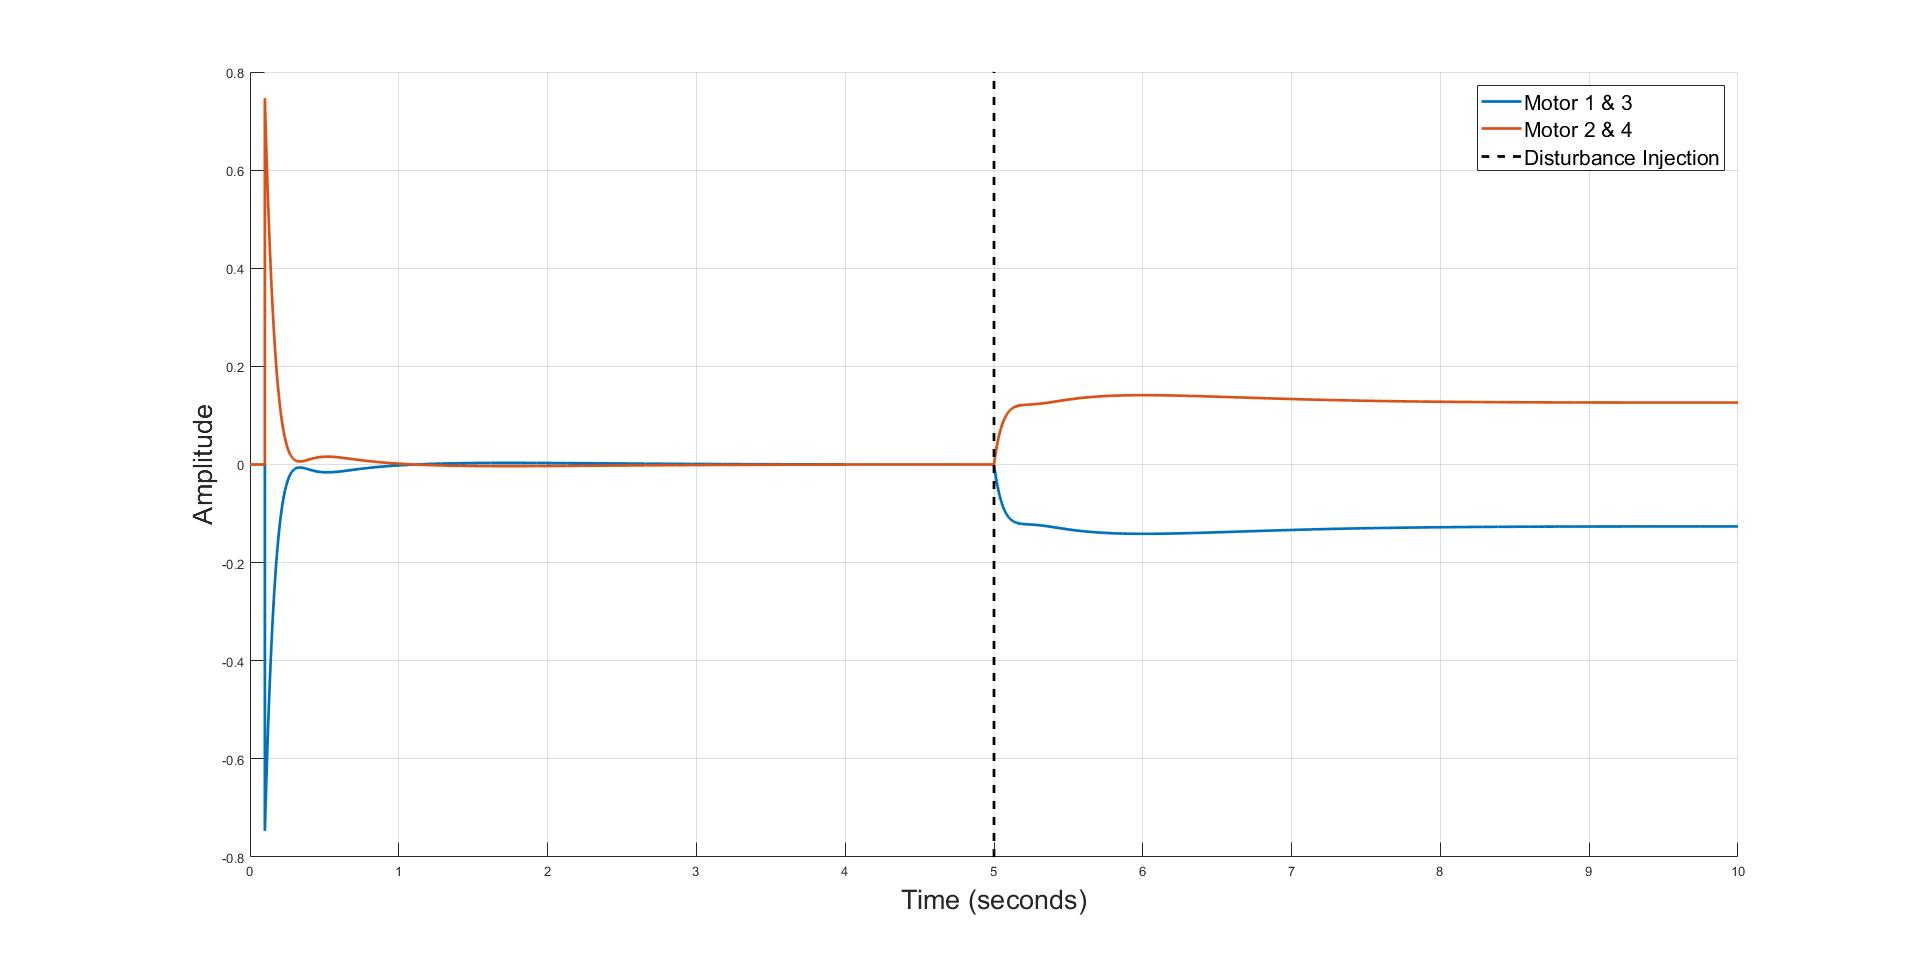
\includegraphics[height = 8cm]{../Design/Matlab/Controllers/pitch_rate_impulse.jpg}
			\caption{Pitch Rate Controller -  Motor Commands}
			\label{IM_PitchRateImpulse}
		\end{figure}
		
		Intuitively it can be strange that the pitching step response produces larger motor outputs than the rolling step. The longer pitch actuator arm would lead one to believe that the pitch system will command lower values of thrust. This is only true for a similar moment. The differing inertias entails that for a rate step response the rolling plant will produce a lower moment impulse as compared to the pitching system. To quantify the effect of the arm length versus the effect of the inertias both can be represented as ratios. The ratio between the roll and pitch arm lengths is $3.73$ where the ratio between the inertias is $6.76$. Therefore the pitch system has to work, ratio metrically, $1.81$ times harder than the rolling system resulting in larger motor thrust outputs.
		
	\subsection{Tilt Angle Controller}
	The tilt angle controller is responsible for controlling the desired roll and pitch angles of the craft. The controller does this by commanding angular rates it calculates from a translational acceleration reference in the earth frame. Using the current angular position, this earth frame acceleration reference is converted to the body frame and used to calculate the error in angular positions for roll and pitch. This error is then fed through a Proportional gain. This section makes reference to Figure \ref{IM_TiltAngleController} and begins by explaining the method used for converting the acceleration reference into desired angular rates.
	
	\begin{figure}[H]
		\centering
		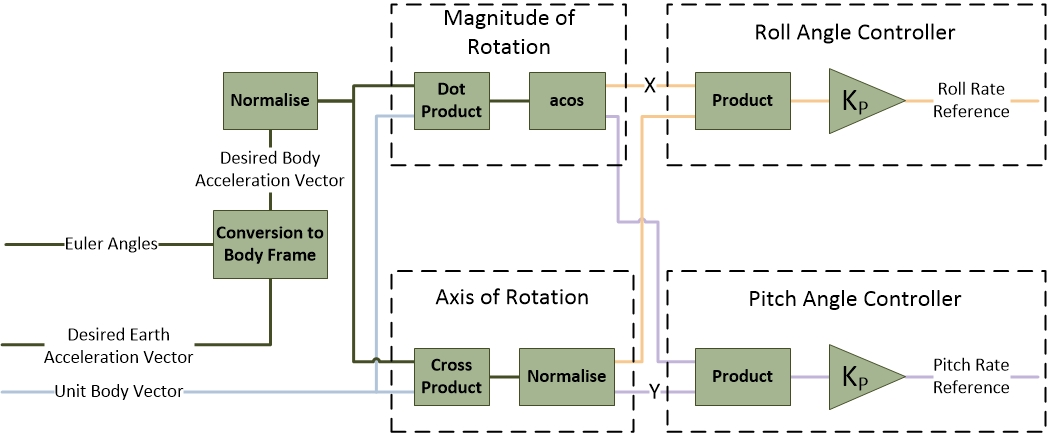
\includegraphics[height = 6.5cm]{../References/Diagrams/TiltAngleController.jpg}
		\caption{Tilt Angle Controller}
		\label{IM_TiltAngleController}
	\end{figure}
		
		\subsubsection{Method of Conversion}	
		The first step to calculating the desired roll and pitch angles is to convert the earth frame set point into a body frame reference. To enable the transformation, a rotation matrix is calculated from the current Euler angles as seen in \eqref{EQ_RotationMatrix}. It is important to mention at this point that in order for accurate alignment, the desired earth acceleration vector must include a gravity component. The desired, now body, acceleration vector is normalised and then compared with a unit body vector. To remove any dependency on yaw, a unit Z body vector is created, which is perfectly aligned with the Z-Axis and thrust generation of the craft. Utilising the dot product shown in \eqref{EQ_DotProduct} the magnitude of the rotation can be calculated. Unit vectors are used, so simply taking the arc cosine of the result will produce the magnitude of rotation. The axis of rotation can subsequently be calculated by using the cross product shown in \eqref{EQ_CrossProduct} and normalising the output to remove any magnitude. Figure \ref{IM_AngleMethod} is used a visual aid for the preceding description.
		
 		\begin{equation}
 		\label{EQ_DotProduct}
 		\vec{a} \, \bigcdot \, \vec{b} = |ab|\,\cos \alpha
 		\end{equation}
 		
 		\begin{equation}
 		\label{EQ_CrossProduct}
 		\vec{a} \, \times \, \vec{b} = \vec{c}
 		\end{equation}
		
		\begin{figure}[H]
			\centering
			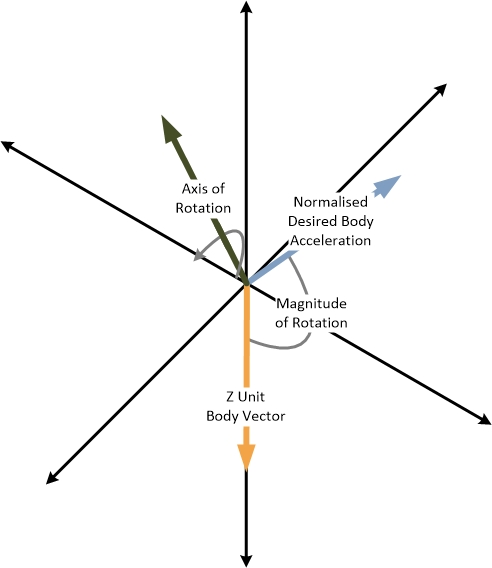
\includegraphics[height = 10cm]{../References/Diagrams/ConversionMethod.jpg}
			\caption{Conversion Technique using Dot and Cross Products}
			\label{IM_AngleMethod}
		\end{figure}
	
		\subsubsection{Roll and Pitch Angle Controllers}
		The linear analysis of the tilt angle controller is done by simplifying the system as shown in Figure \ref{IM_RollAngleLoop}. The additional time required to calculate the setpoints and the rotation matrix can be considered in the design by ensuring sufficient phase margin. As mentioned in the rate controller section, the outer controllers are limited by the inner loop bandwidth. The roll and pitch angle controllers must account for this by having a slower system with less bandwidth. For practical systems, the ratio between the inner and outer loop should be in the region of $2 - 4$. The inner rate controller includes an integrator term and can handle disturbances, thus allowing for a less complex angle control law. 
		
		\begin{figure}[H]
			\centering
			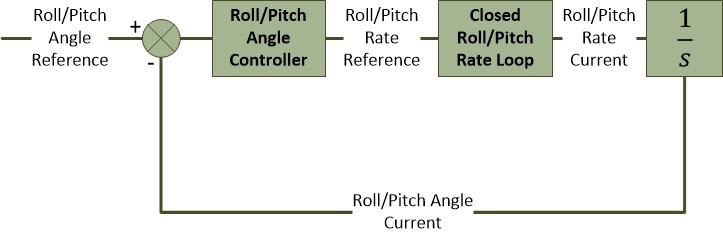
\includegraphics[height = 3.5cm]{../References/Diagrams/RollPitchAngleLoop.jpg}
			\caption{Roll and Pitch Angle Simplified Closed Loops}
			\label{IM_RollAngleLoop}
		\end{figure}
		
		The roll angle loop's frequency response is shown in the Bode plot in Figure \ref{IM_RollAngleControlBode}. Unity feedback is compared against the chosen controller. The integration between rate and position increases the phase in the lower frequencies producing sufficient phase, allowing for a simple Proportional (P) control law in the angle loop. The final phase margin is $78$\textdegree. The controller adds a bit more gain than unity feedback and increases the bandwidth while pushing the crossover frequency to $1.26$\,rad/s. There is now a ratio of $3.8$ between the inner and outer loop. From observation there is still more room for a faster system and increased bandwidth. However, the damping decreases as the system is pushed harder creating a need for more complex control law, with little gain benefit.
		
		\begin{figure}[H]
			\centering
			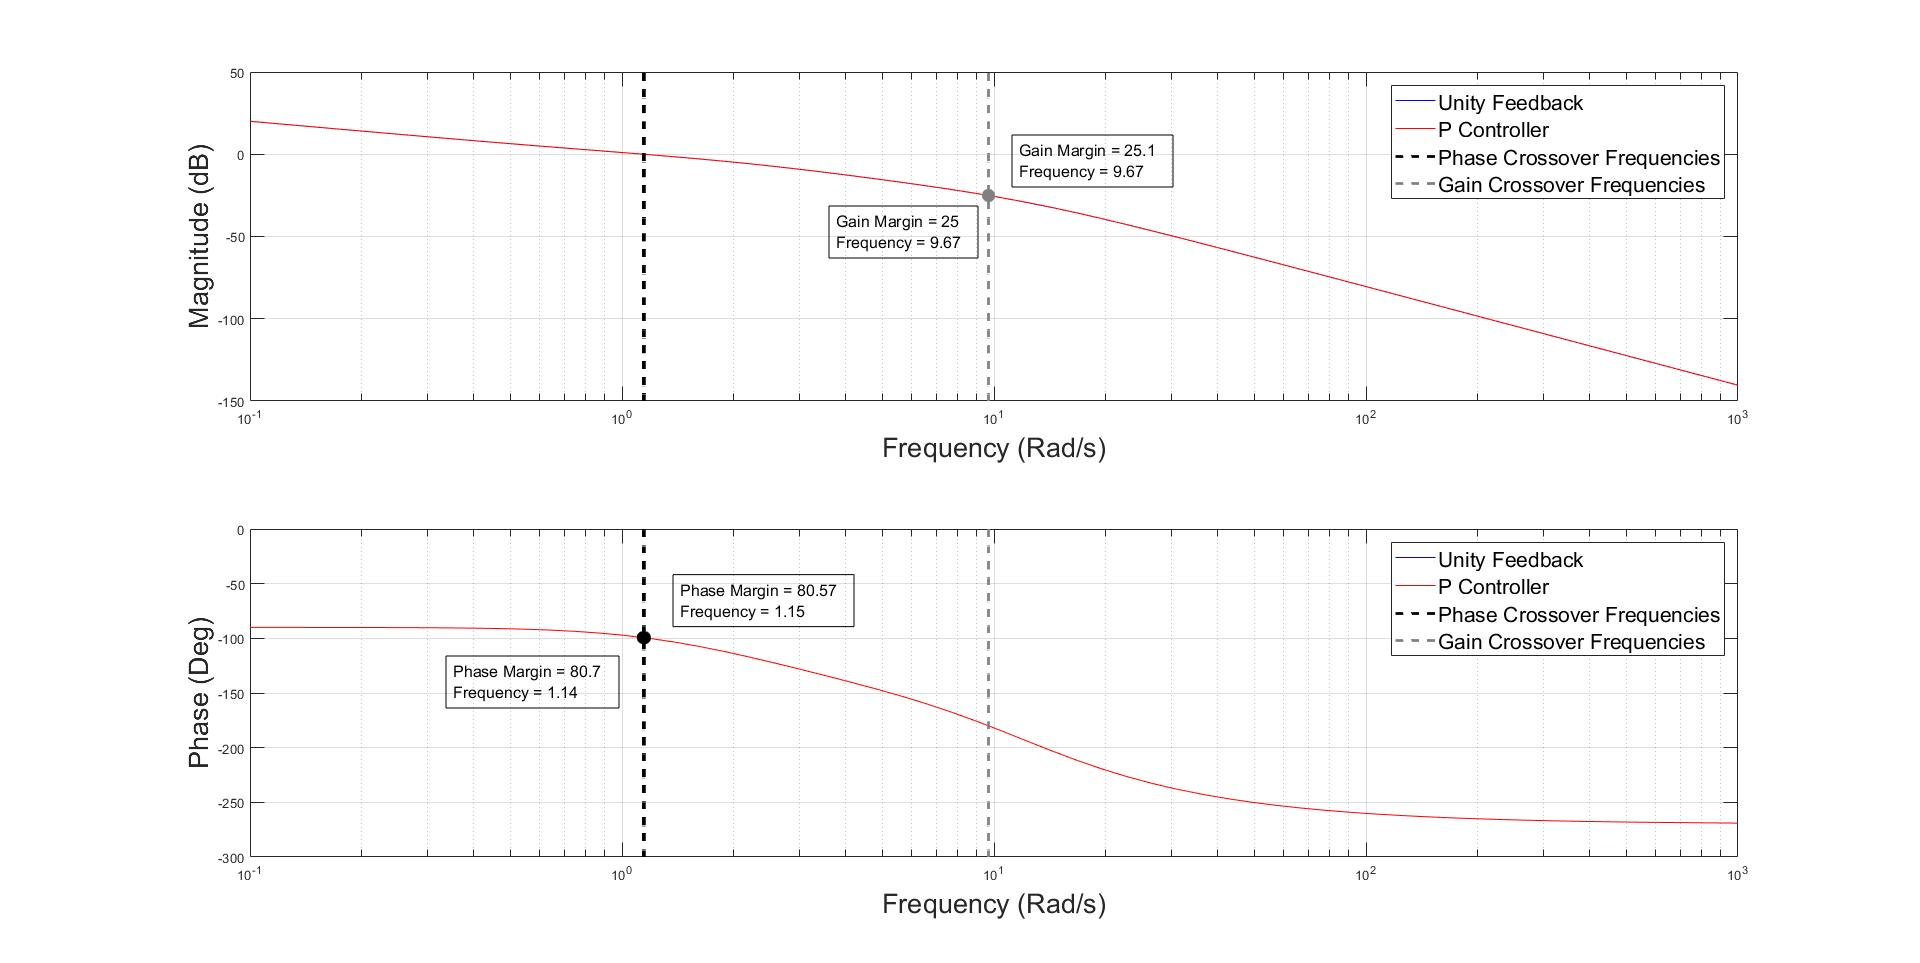
\includegraphics[height = 8cm]{../Design/Matlab/Controllers/roll_angle_bode.jpg}
			\caption{Roll Angle Controller -  Bode Plots}
			\label{IM_RollAngleControlBode}
		\end{figure}
	
		\subsubsection{Tilt Angle Controller Discussion}
		The time domain response of the system is evaluated and discussed next. To draw a comparison between the roll and pitch systems their step responses are plotted together in Figure \ref{IM_RollAngleStep}. As desired, the roll and pitch angle transient responses are almost identical. The final rise time for both systems is $1.65$\,s and they both successfully have zero steady state error. The same disturbances used in the rate loop are applied to this system at $10$\,s. As shown, both systems handle the disturbance successfully. Although, as expected, the pitch system deviates less from the reference.
		
		\begin{figure}[H]
			\centering
			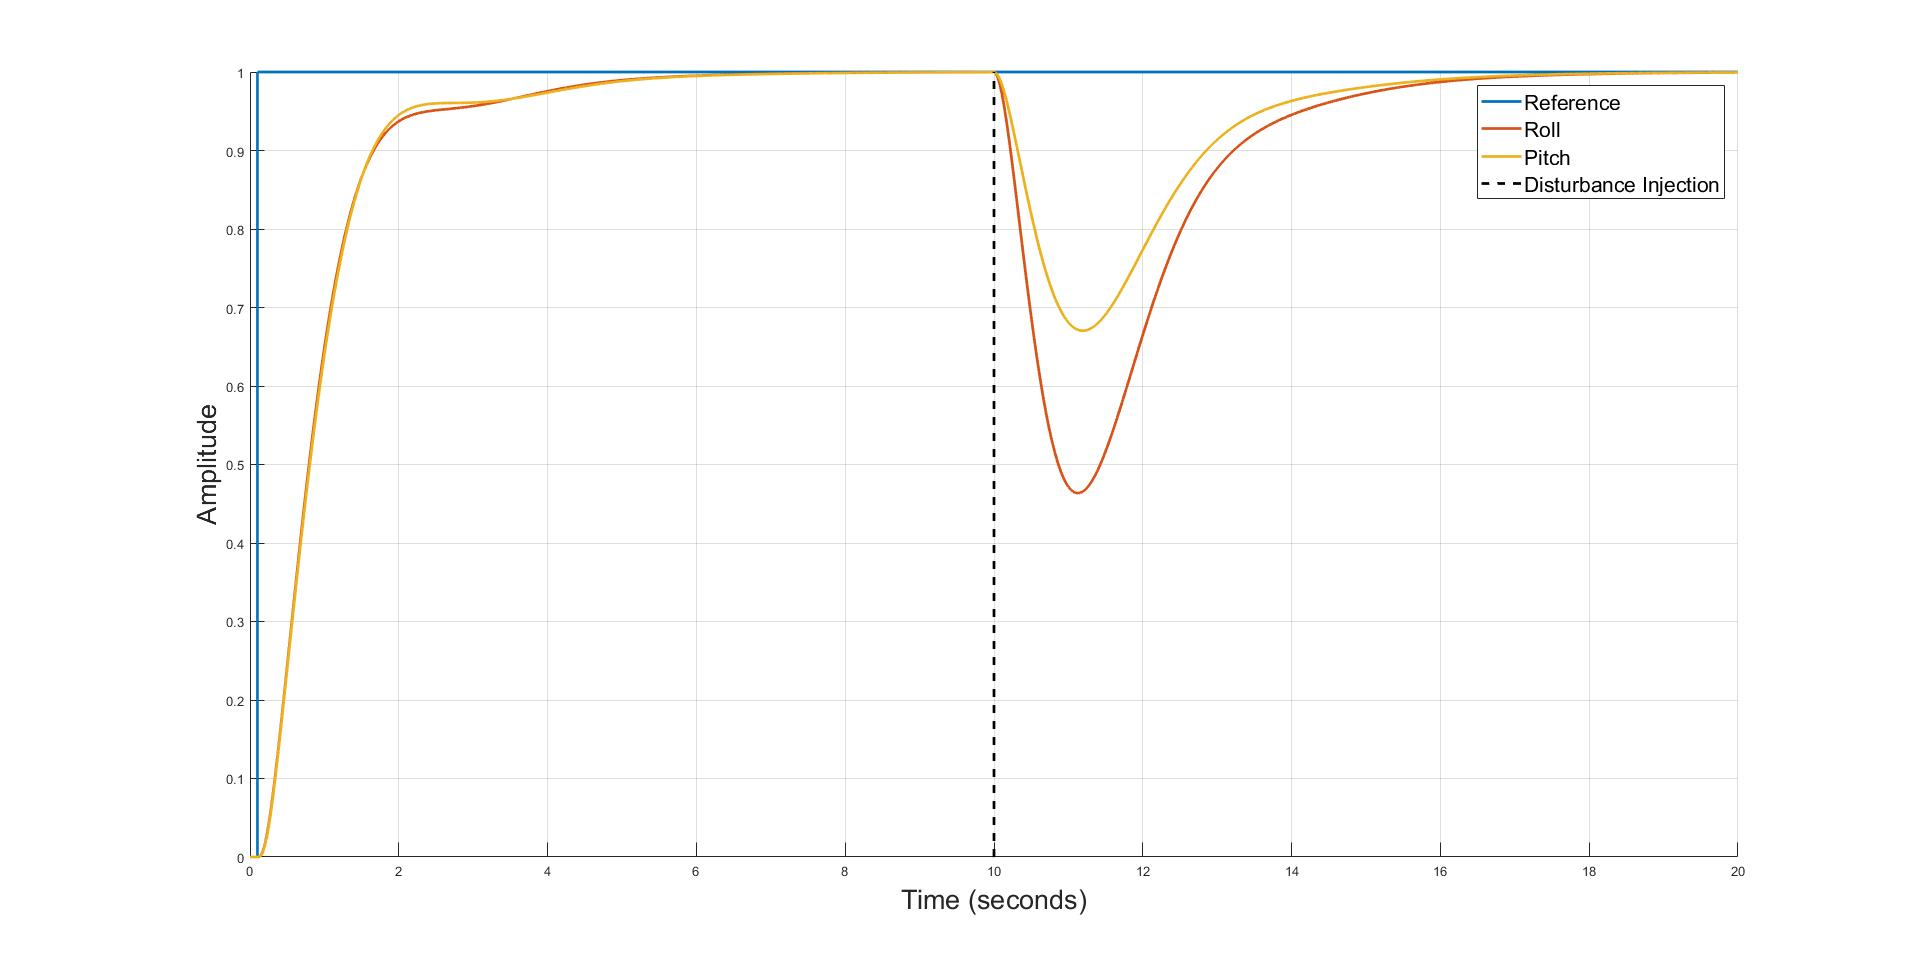
\includegraphics[height = 8cm]{../Design/Matlab/Controllers/roll_pitch_angle_step.jpg}
			\caption{Roll and Pitch Angle Controller -  Step Responses}
			\label{IM_RollAngleStep}
		\end{figure}
		
		Finally the commands sent to the motors are evaluated in Figures \ref{IM_RollAngleImpulse} and \ref{IM_PitchAngleImpulse}. The maximum thrust commanded by the pitch system is just less than $0.8$\,N. As expected the roll system commands a lower maximum of $0.57$\,N.
		
		\begin{figure}[H]
			\centering
			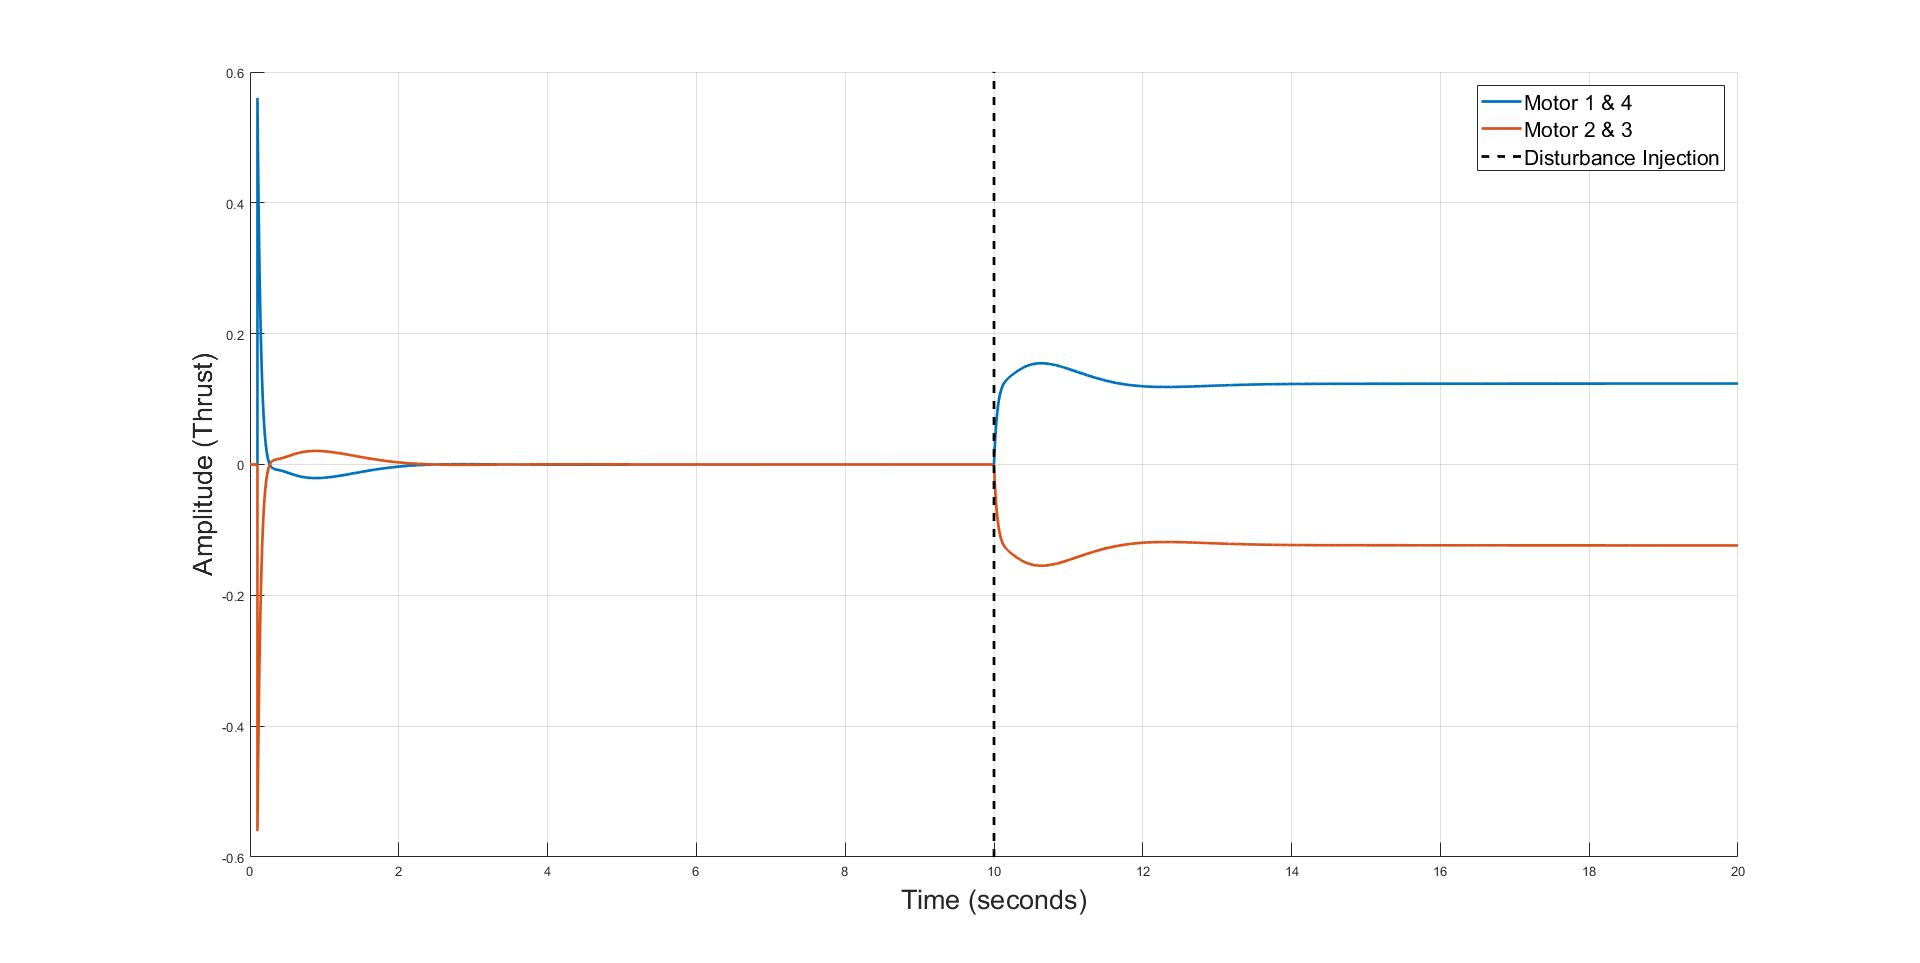
\includegraphics[height = 8cm]{../Design/Matlab/Controllers/roll_angle_impulse.jpg}
			\caption{Roll Angle Controller -  Motor Commands}
			\label{IM_RollAngleImpulse}
		\end{figure}
				
		\begin{figure}[H]
			\centering
			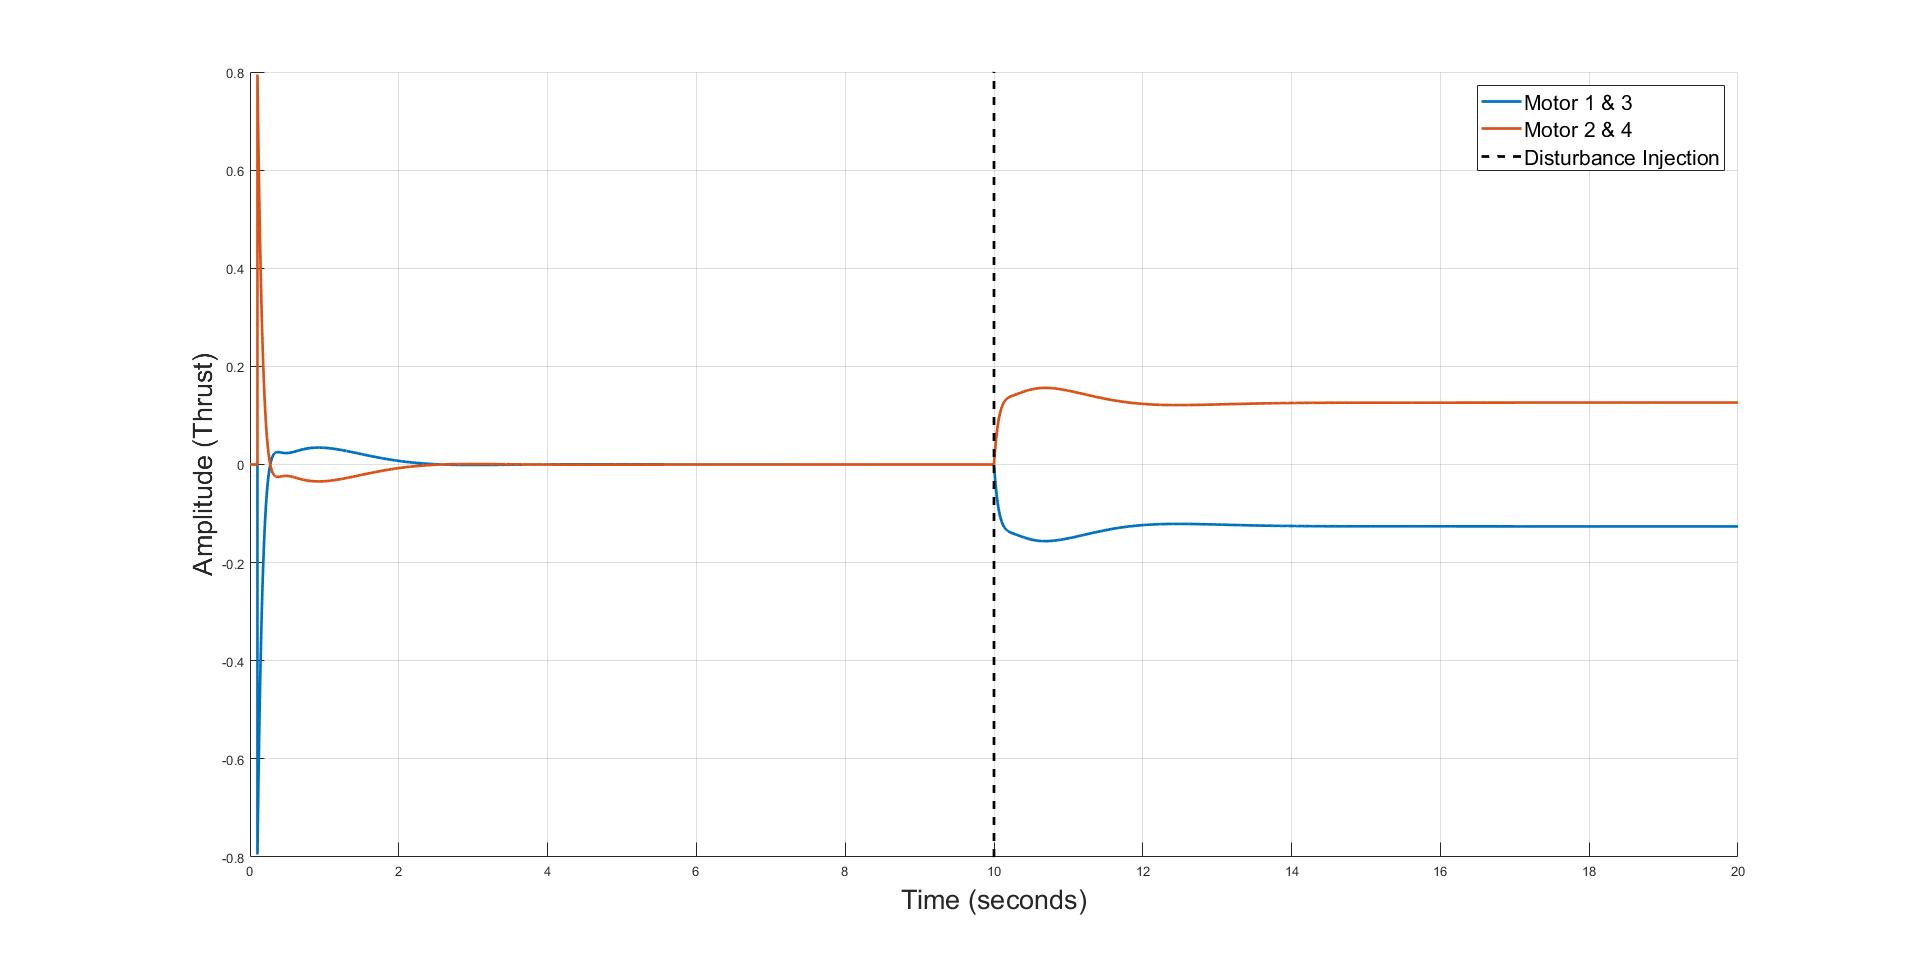
\includegraphics[height = 8cm]{../Design/Matlab/Controllers/pitch_angle_impulse.jpg}
			\caption{Pitch Angle Controller -  Motor Commands}
			\label{IM_PitchAngleImpulse}
		\end{figure}
	
	\subsection{Linear Velocity Control}
	This section follows the design of the linear velocity controller. This controller is responsible for controlling the translational velocities of the craft along the North and East axis. This controller will receive a reference from the outer position loop and feed an acceleration command to the tilt angle controller. The tilt angle controller implementation successfully abstracts the angular position from the acceleration reference. However, the relationship between the pitch angle of the craft and North acceleration reference still requires a linearisation for the controller design. 
	
	For simplification the craft is assumed to be travelling at a maintained height in a Northern direction, with zero heading. The relationship between Northern acceleration of the craft can then be defined trigonometrically by the pitch angle of the craft as seen in \eqref{EQ_LinearNorthVel}. 
	
	\begin{eqnarray}
	\ddot{N} &=& g\times \tan \theta \label{EQ_LinearNorthVel}
	\end{eqnarray}

	At low angles, which is expected for the craft, $\tan \theta$ can be approximated to $\theta$ allowing for the linearisation seen in \eqref{EQ_LinearNorthVel2} and \eqref{EQ_LinearNorthVel4}. The closed loop diagram can then also be simplified as shown in Figure\ref{IM_NorthVelocityLoop}.
	
	\begin{eqnarray}
	\ddot{N} &\approx& g\times \theta \label{EQ_LinearNorthVel2}\\\label{EQ_LinearNorthVel3}
	\theta 	&\approx& \frac{\ddot{N}}{g} \label{EQ_LinearNorthVel4}
	\end{eqnarray}
	
	\begin{figure}[H]
		\centering
		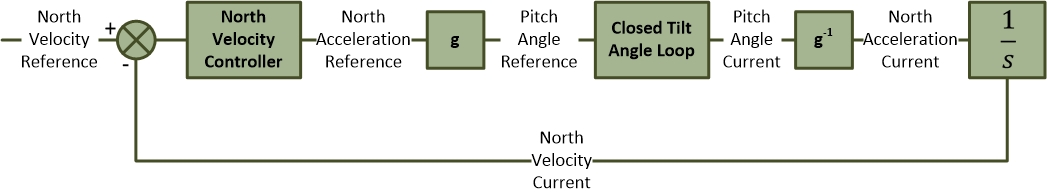
\includegraphics[height = 2.9cm]{../References/Diagrams/NorthVelocityLoop.jpg}
		\caption{North East Simplified Closed Loops}
		\label{IM_NorthVelocityLoop}
	\end{figure}
	
	The allowed bandwidth of the linear velocity controller is limited by the bandwidth of the tilt angle controller. The free integrator in the linear velocity loop will ensure that the system will track a set point with zero steady state error. However, there are expected disturbances which require more complex control than proportional control to reject. The Bode plots in Figure \ref{IM_NorthVelControlBode} assist with the design by allowing easy analysis of phase and gain in the system.
	
	A traditional PI architecture increases the low frequency gain, however was not suitable due to the loss in phase and damping. Instead a lag compensator could be designed to limit the overshoot while enabling some disturbance rejection. The process of designing the lag compensator under went the following steps. First a proportional controller is designed to achieve the desired bandwidth, $\omega_{des}$. The zero of the compensator is then placed far enough to negate any effect on the bandwidth. The pole has been placed to optimise both limiting overshoot and enabling disturbance rejection.
	
	As desired the P and lag controlled systems exhibit the same crossover frequency bandwidth and negligibly different high gain profiles. Both the lag compensator and the PI controller increase the low bandwidth gain at the cost of some phase. However, the phase benefits of the lag compensator compared to the PI controller can be seen clearly. The final system is designed to have a crossover frequency of $0.42$\,rad/s and a phase margin of $65$\textdegree. This bandwidth is a ratio $2.7$ slower than the slowest loop in the tilt angle controller.
			
	\begin{figure}[H]
		\centering
		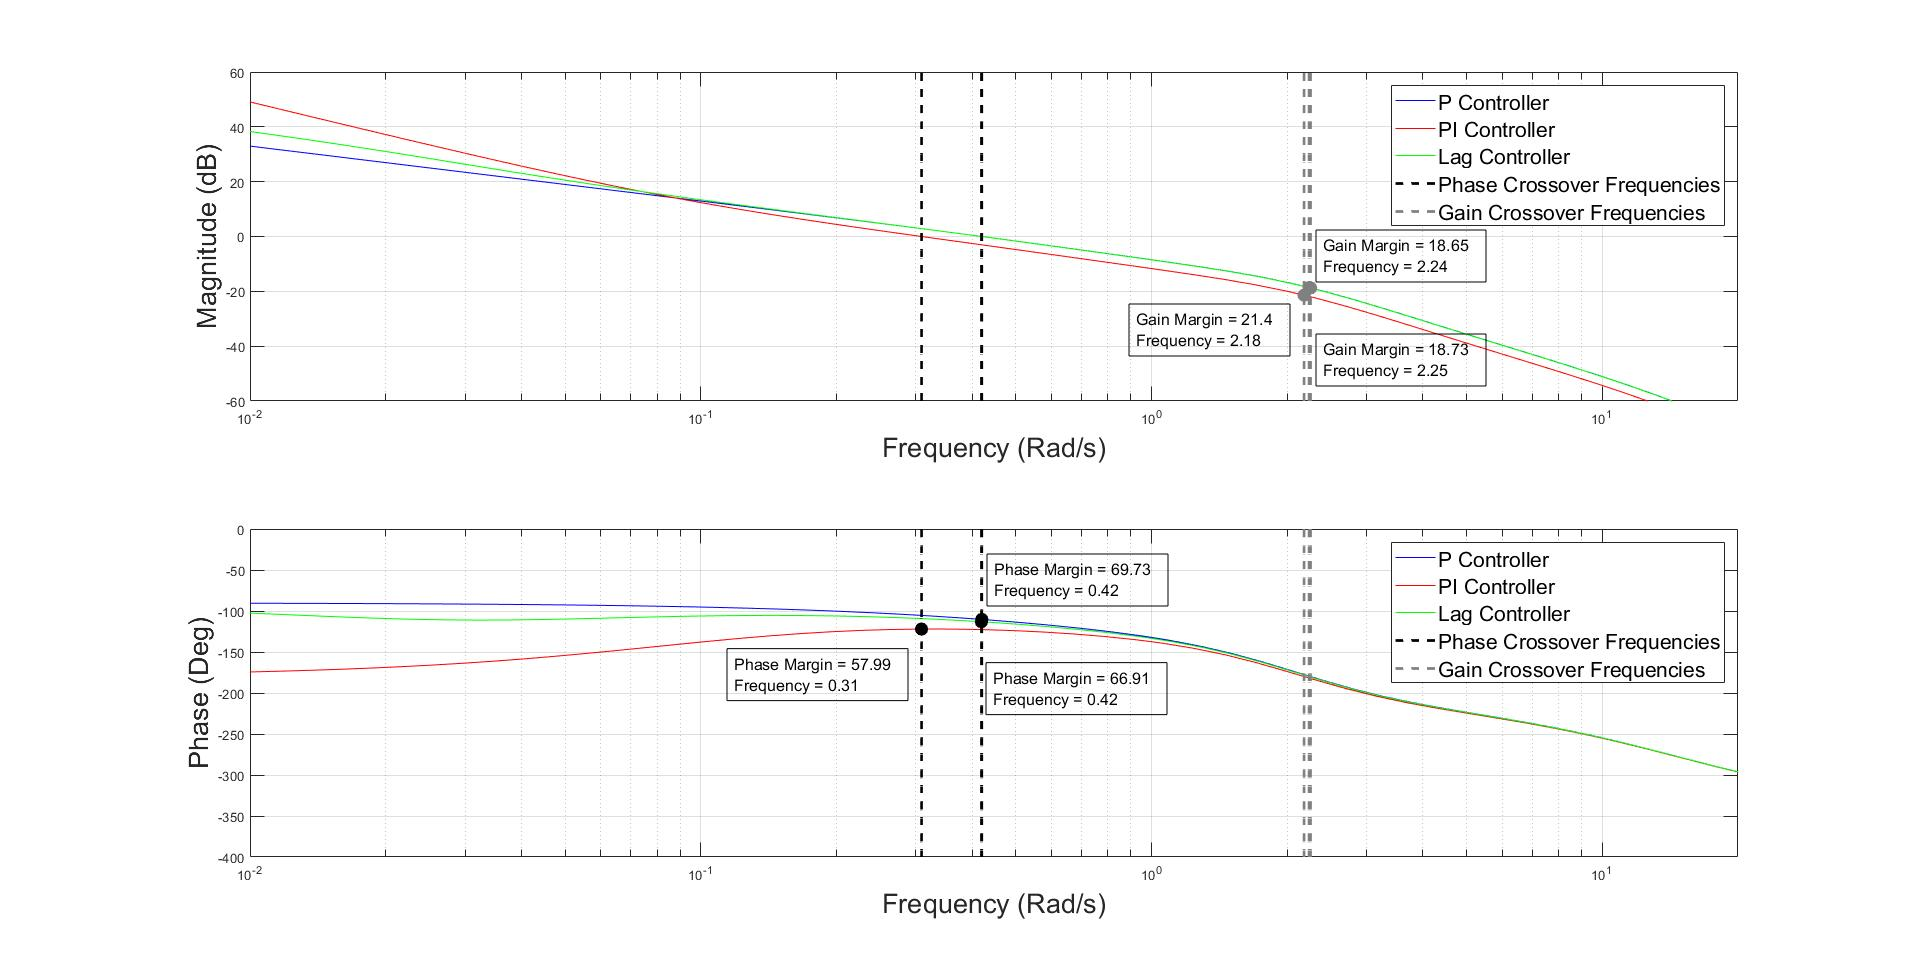
\includegraphics[height = 8cm]{../Design/Matlab/Controllers/north_velocity_bode.jpg}
		\caption{North Velocity Controller -  Bode Plots}
		\label{IM_NorthVelControlBode}
	\end{figure}
	
	The final placement of the lag compensator can be shown on the root locus in Figure \ref{IM_NorthVelControlRoot}. The compensator zero has been placed at $\dfrac{\omega_{des}}{10}$ with the pole a factor of $4$ slower.
	
	\begin{figure}[H]
		\centering
		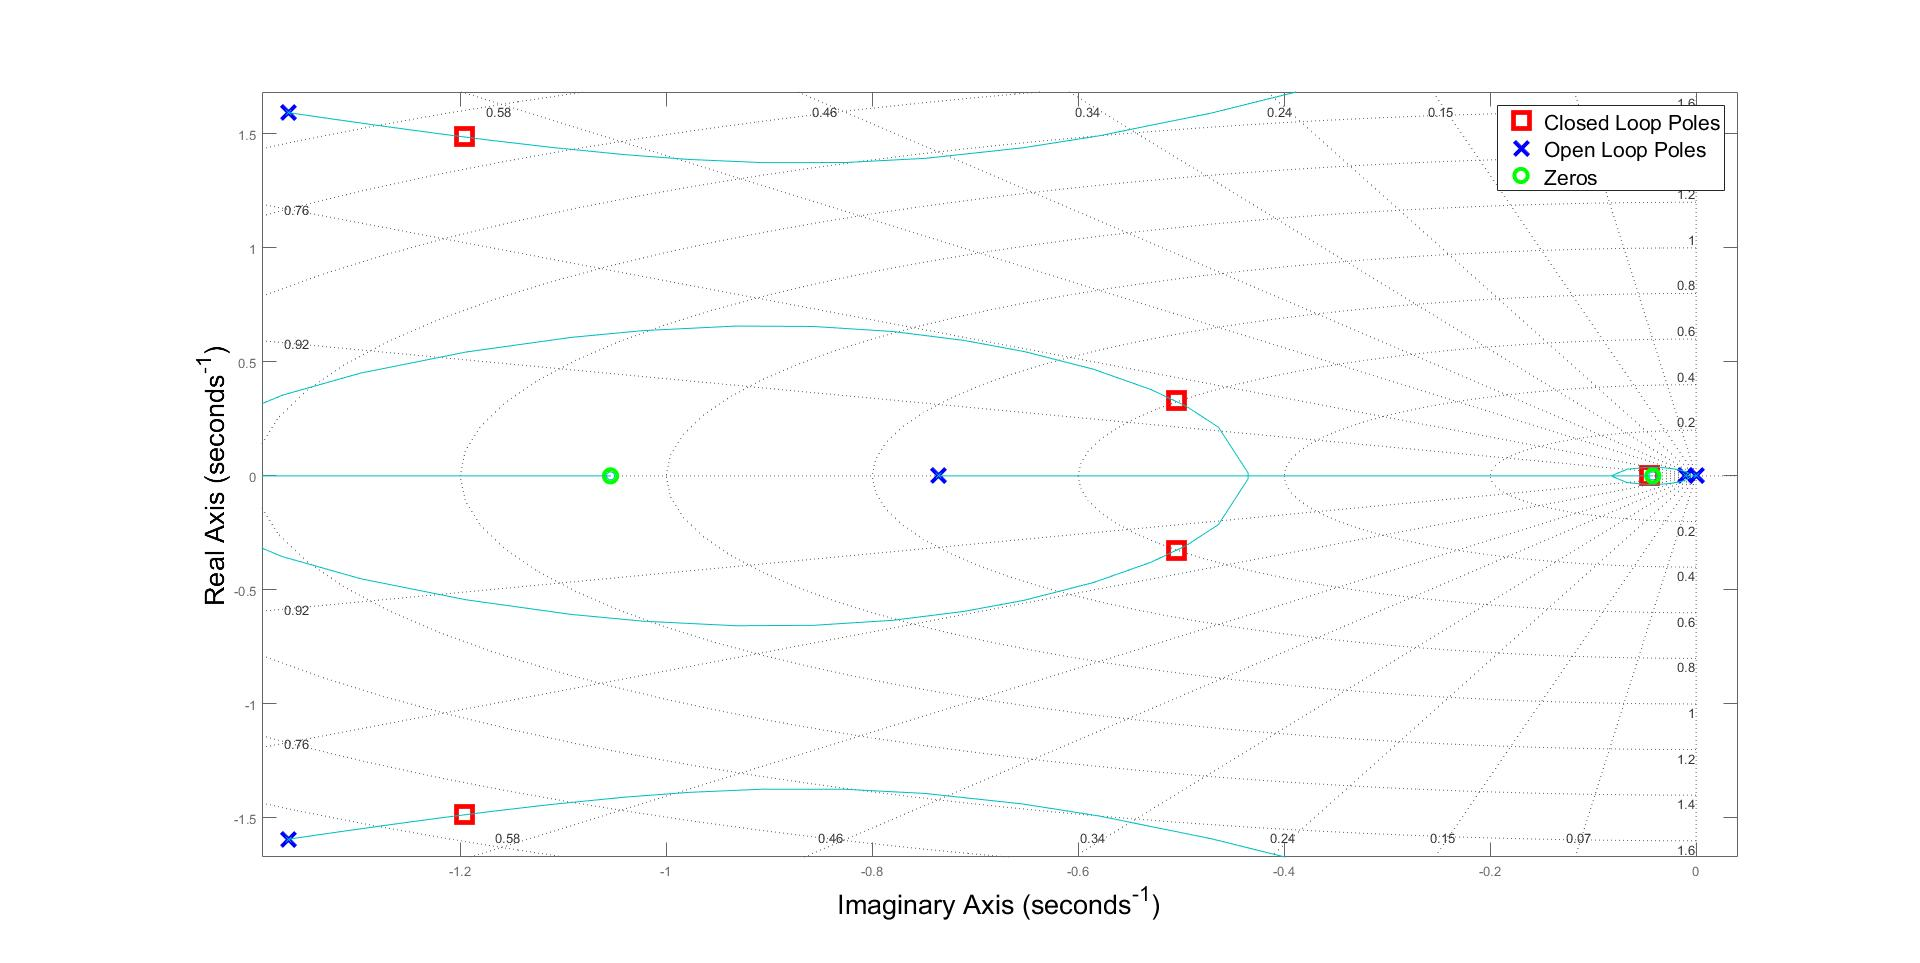
\includegraphics[height = 8cm]{../Design/Matlab/Controllers/north_velocity_root.jpg}
		\caption{North Velocity Controller -  Root Locus Plot}
		\label{IM_NorthVelControlRoot}
	\end{figure}	
	
		\subsubsection{Linear Velocity Controller Discussion}
		The three controllers all exhibit a stable dynamic response, the differences in gain and phase were identified and discussed in the Bode plot. The time domain responses and differences can now be evaluated and discussed. The step response of the P, PI and lag controllers are shown in Figure \ref{IM_NorthVelControlStep}. The proportional controller has a fast transient response with a rise time of $3.3$\,s. The P controller exhibits good phase margin and shows little overshoot. The lose in phase of the PI controller presents itself as a large overshoot of $20$\%. The integrator introduces a long tail into the system and slows the transient response to a rise time of $4.9$\,s. The lag compensator has some overshoot and a very similar transient response to the P controller.
		
		\begin{figure}[H]
			\centering
			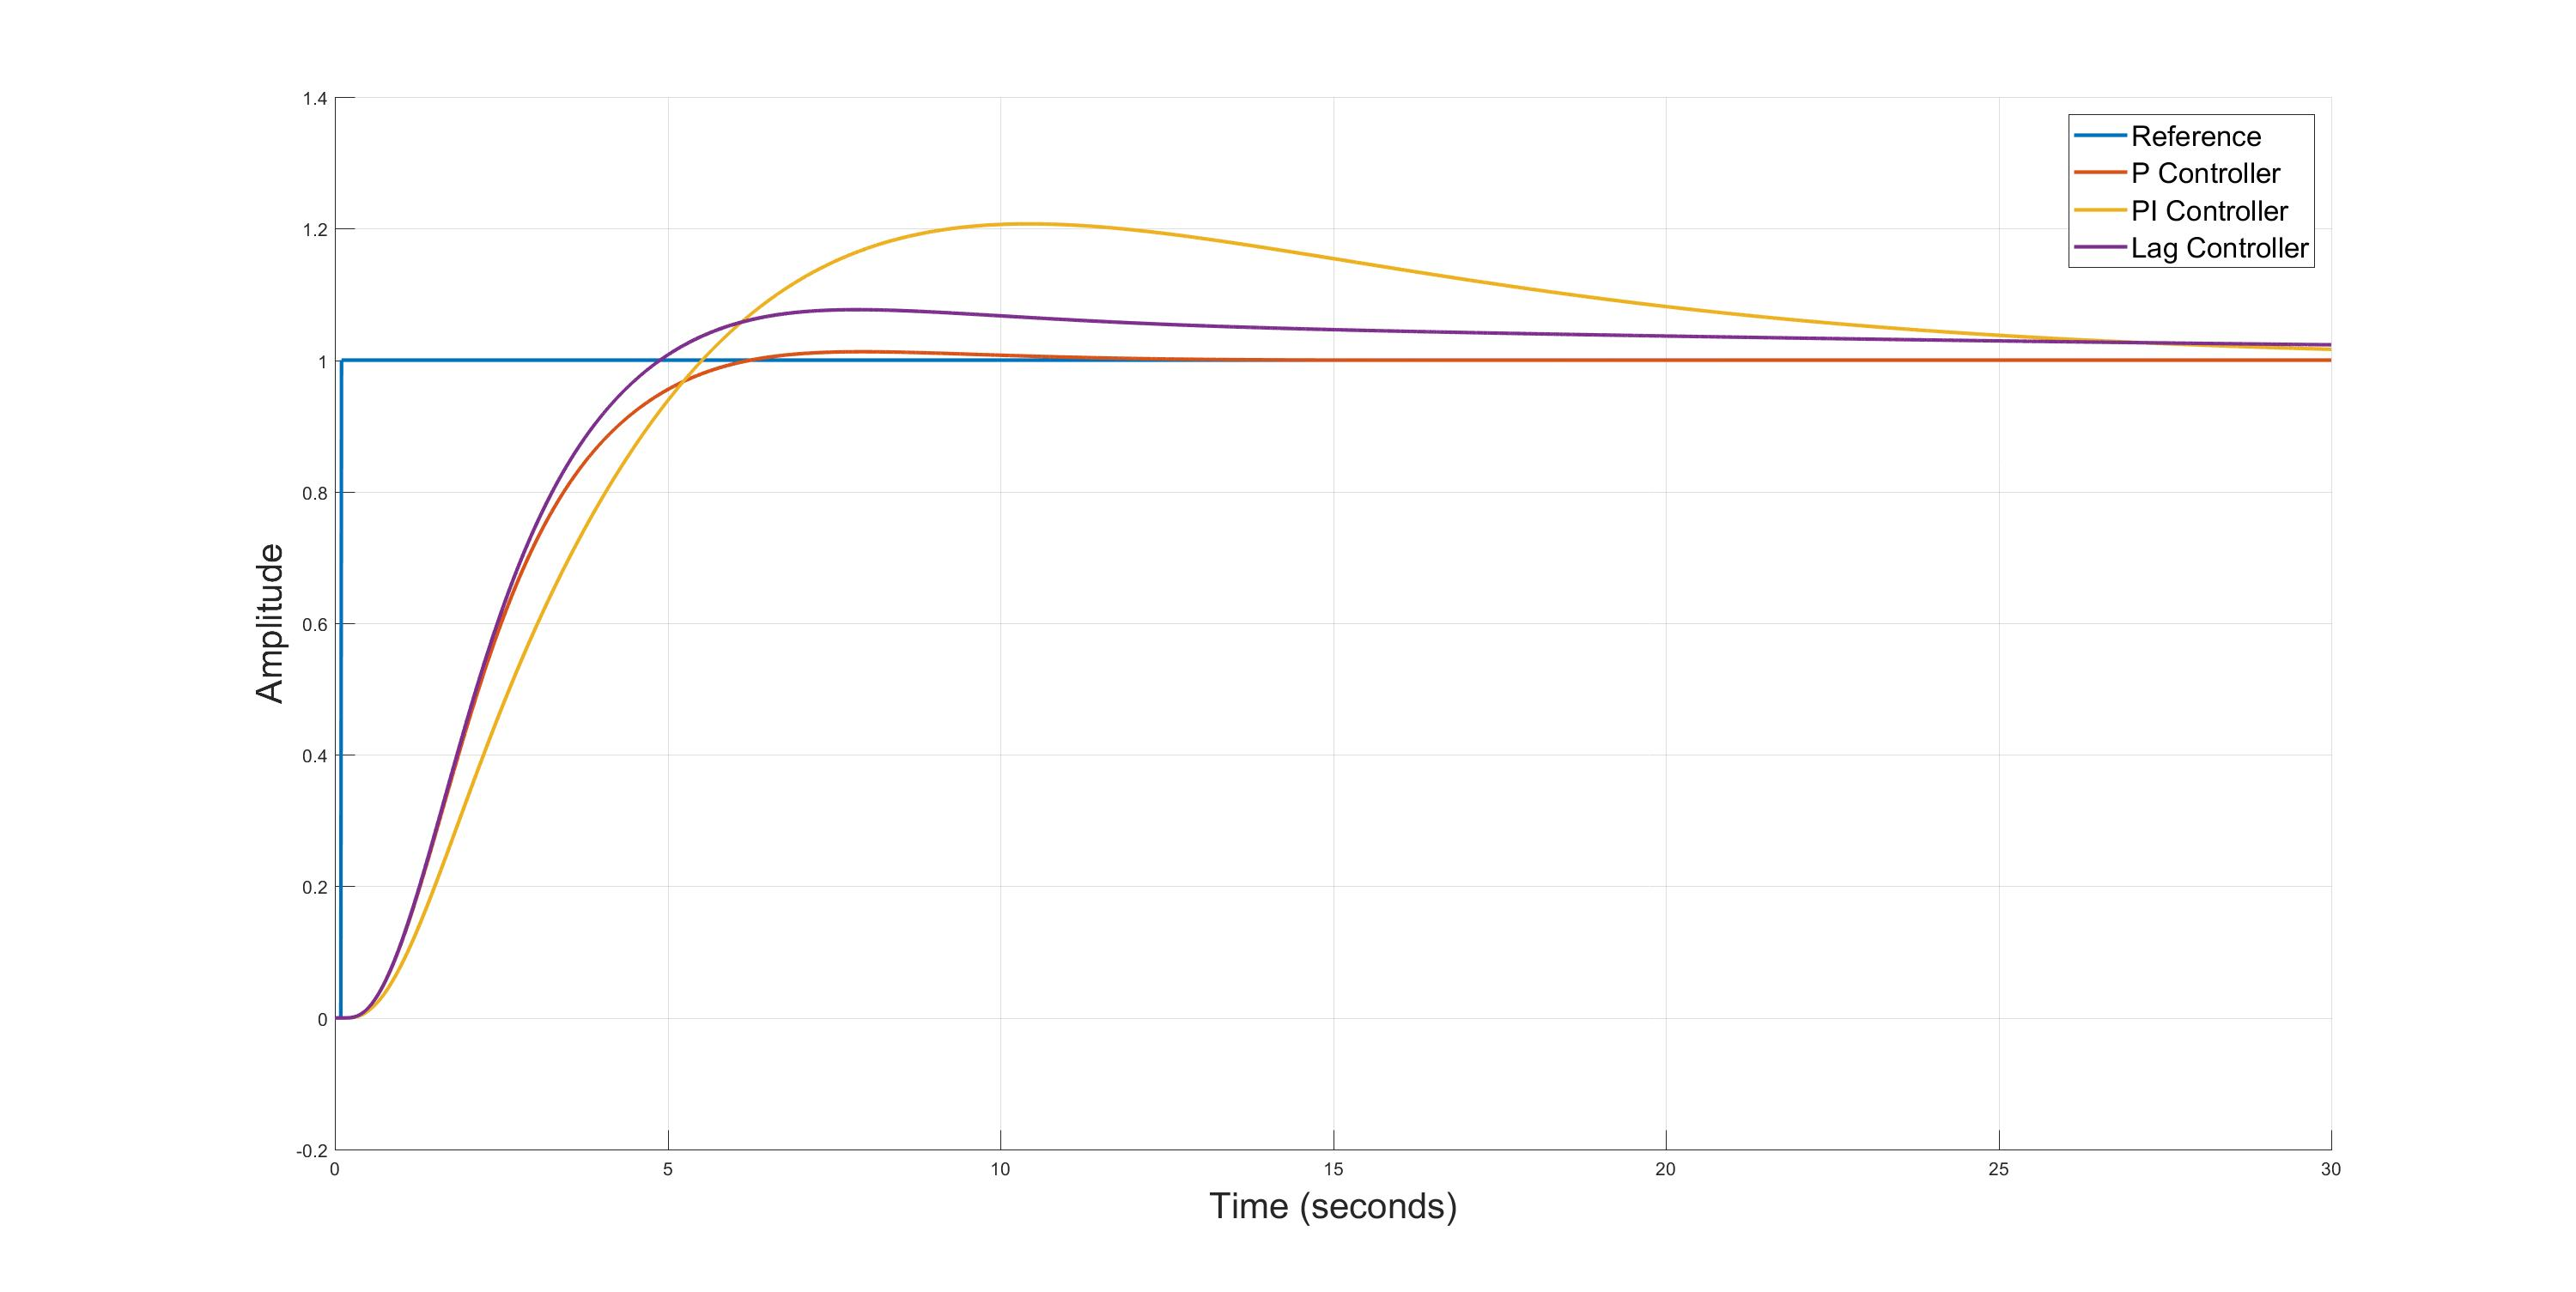
\includegraphics[height = 8cm]{../Design/Matlab/Controllers/north_velocity_step.jpg}
			\caption{North Velocity Controller -  Step Responses}
			\label{IM_NorthVelControlStep}
		\end{figure}	
		
		The benefit of the lag compensator over th P controller can be seen when a disturbance is introduced into the system. Figure \ref{IM_NorthVelControlDistStep} is used to show the effect of a constant disturbance in the system by adding an external force at $30$\,s. The P controller is unable to reject the disturbance. The increased low bandwidth gain of the lag compensator manages to reduce the disturbance and as expected the PI controller successfully rejects the disturbance completely.
	
		\begin{figure}[H]
			\centering
			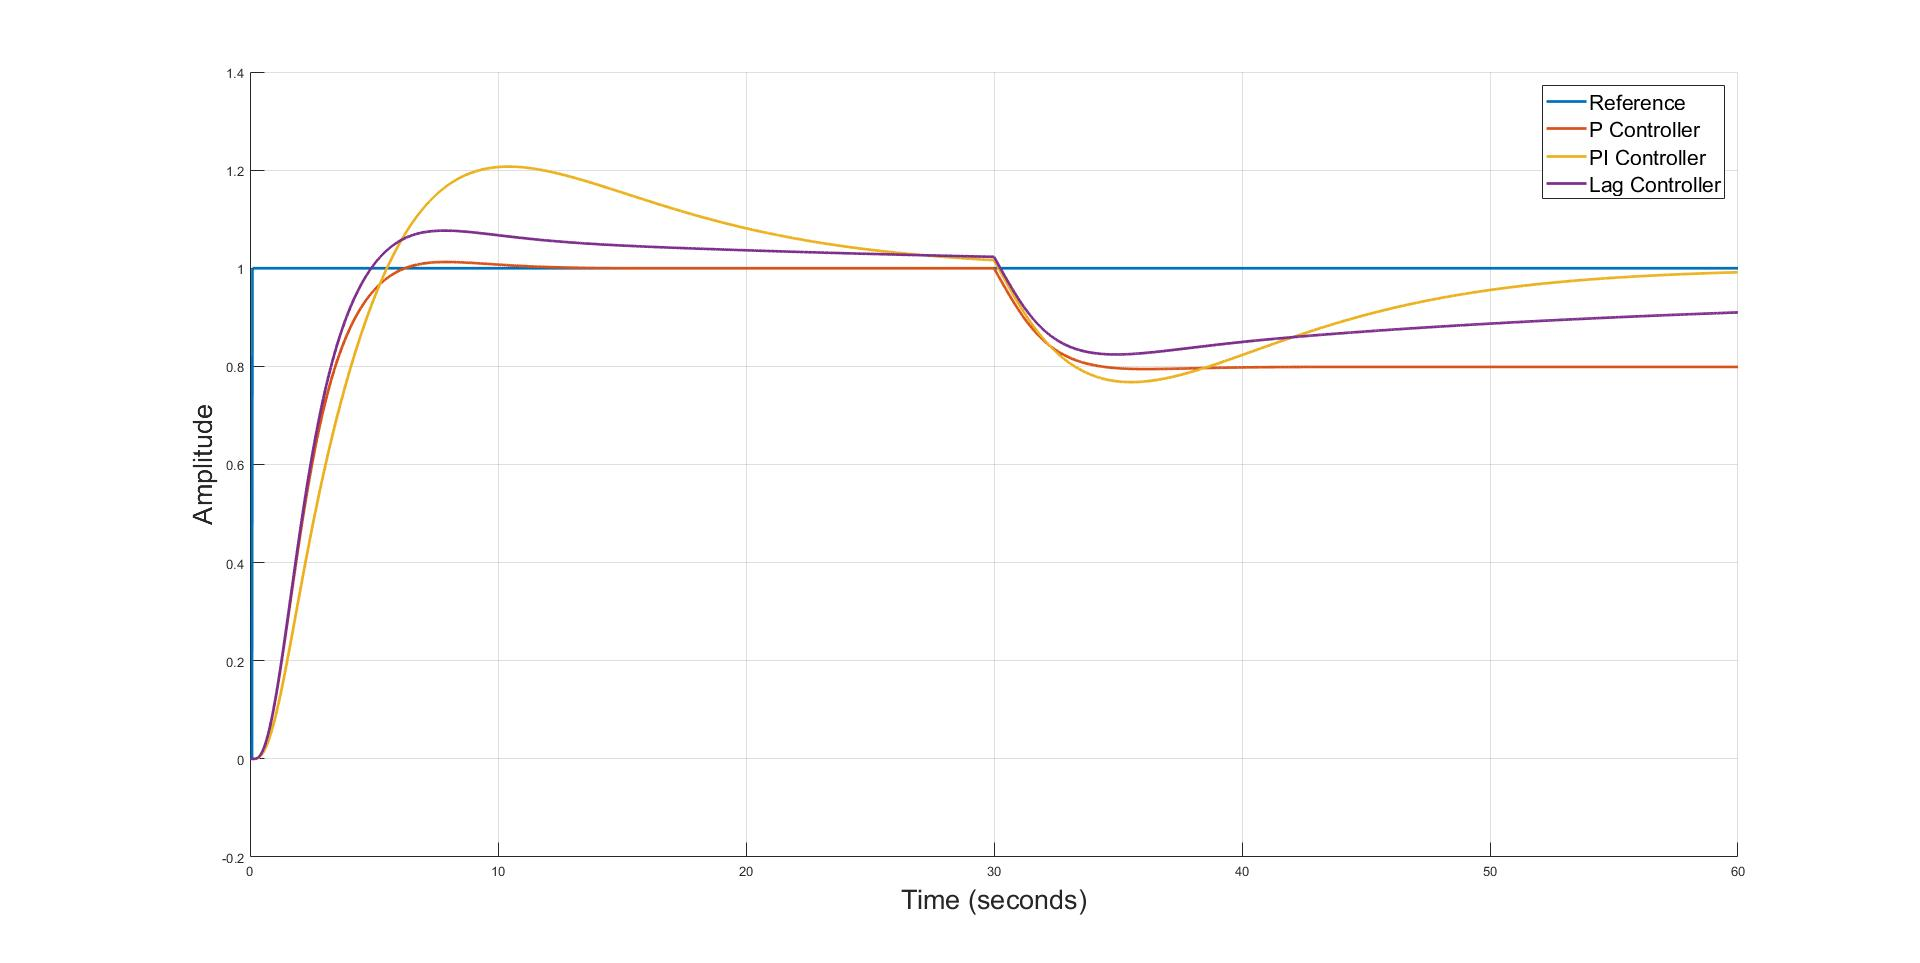
\includegraphics[height = 8cm]{../Design/Matlab/Controllers/north_velocity_stepd.jpg}
			\caption{North Velocity Controller -  Step Responses With a Disturbance}
			\label{IM_NorthVelControlDistStep}
		\end{figure}	
	
	\subsection{Global Position Tracking Control}
	The position controller is the most outer loop of the horizontal controller and will be fed a reference from a waypoint generator or some other, high level flight strategy. There is sufficient disturbance rejection in the inner loops allowing the position controller to use a simple proportional controller. The final bandwidth should utilise the full potential of the inner loop velocity system. The craft should approach a set point steadily and with little overshoot, the final system should thus be well damped.
	
	The Bode plot in Figure \ref{IM_NorthPosControlBode} is used for the design as it easily shows the phase and gain margins of the system. The plant is on the edge of stability and is compared with a controlled system utilising a P controller. The proportional gain is adjusted until there is sufficient phase margin of $69$\textdegree and gain margin of $17$\,dB. The final cross over frequency is $0.16$\,rad/s, creating a ratio of $2.6$ between the inner and outer loop.
	
	\begin{figure}[H]
		\centering
		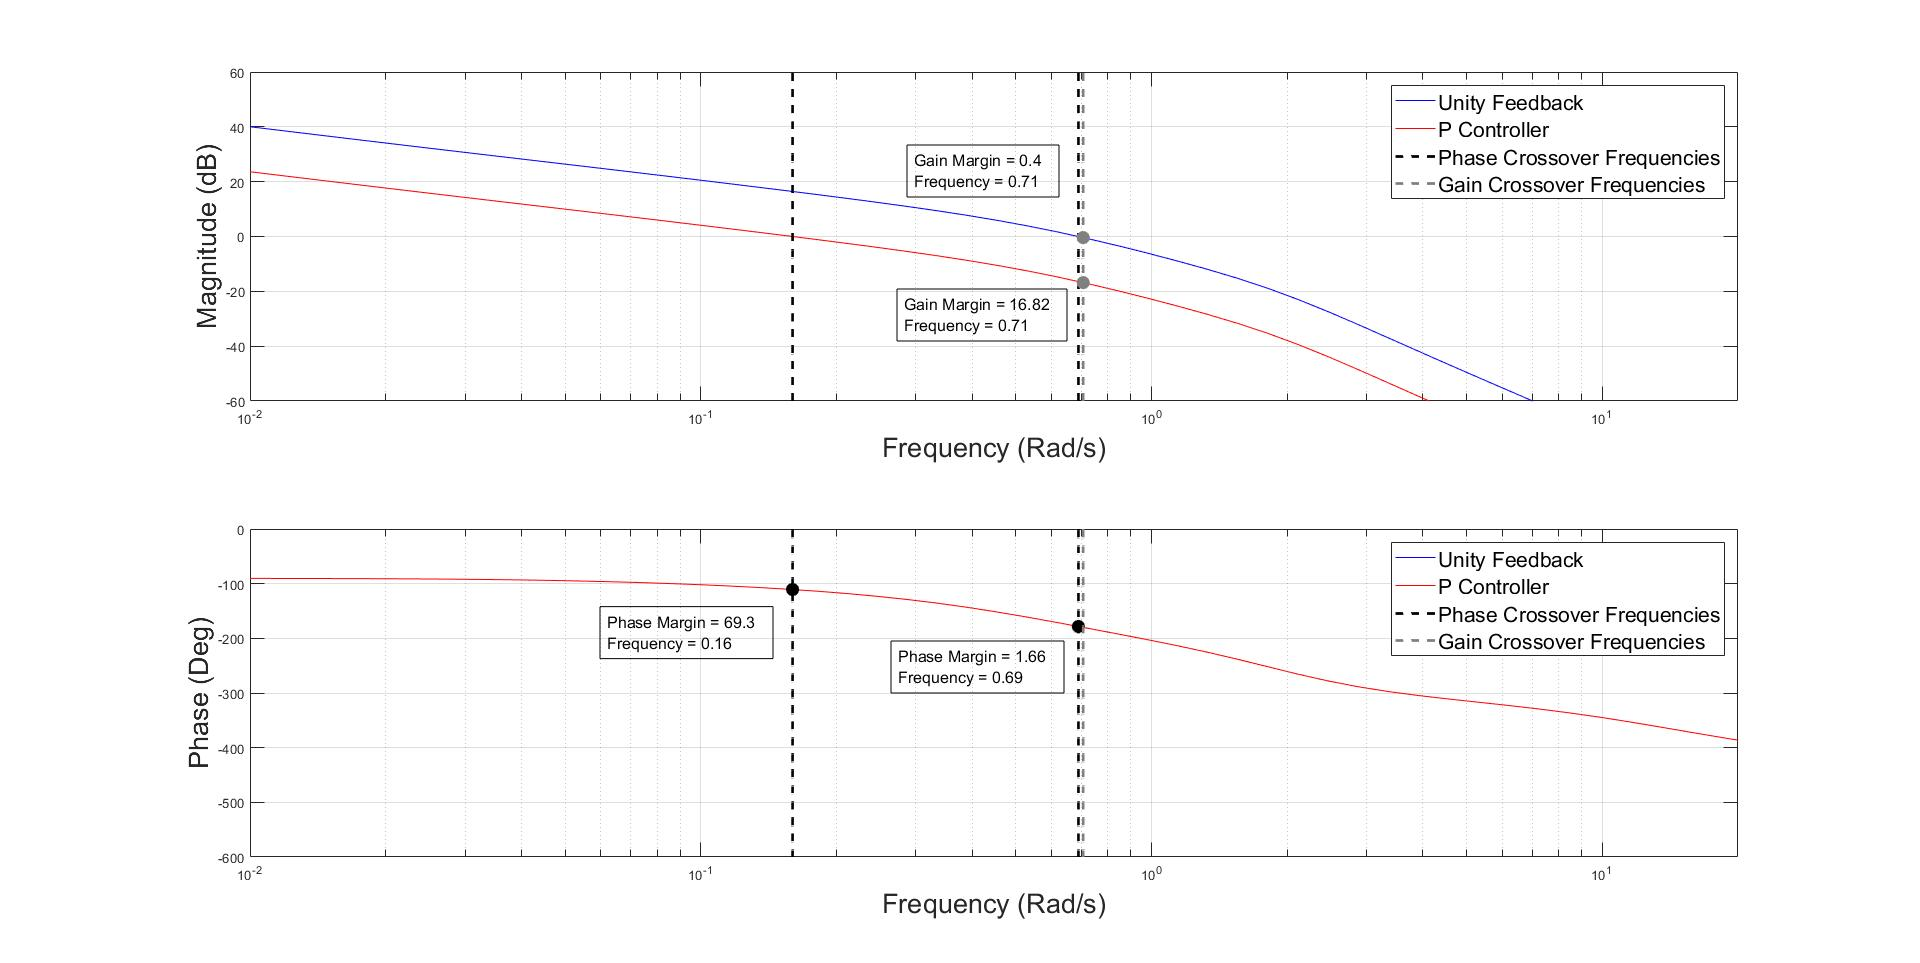
\includegraphics[height = 8cm]{../Design/Matlab/Controllers/north_position_bode.jpg}
		\caption{North Position Controller -  Bode Plots}
		\label{IM_NorthPosControlBode}
	\end{figure}
	
		\subsubsection{Position Controller Discussion}
		The proportional gain increase stability in the system and reduces the crossover frequency. Figure \ref{IM_NorthPosControlStep} represents the step response of the system. The system is shown to be well damped with no oscillatory motion in the response. 
		
		\begin{figure}[H]
			\centering
			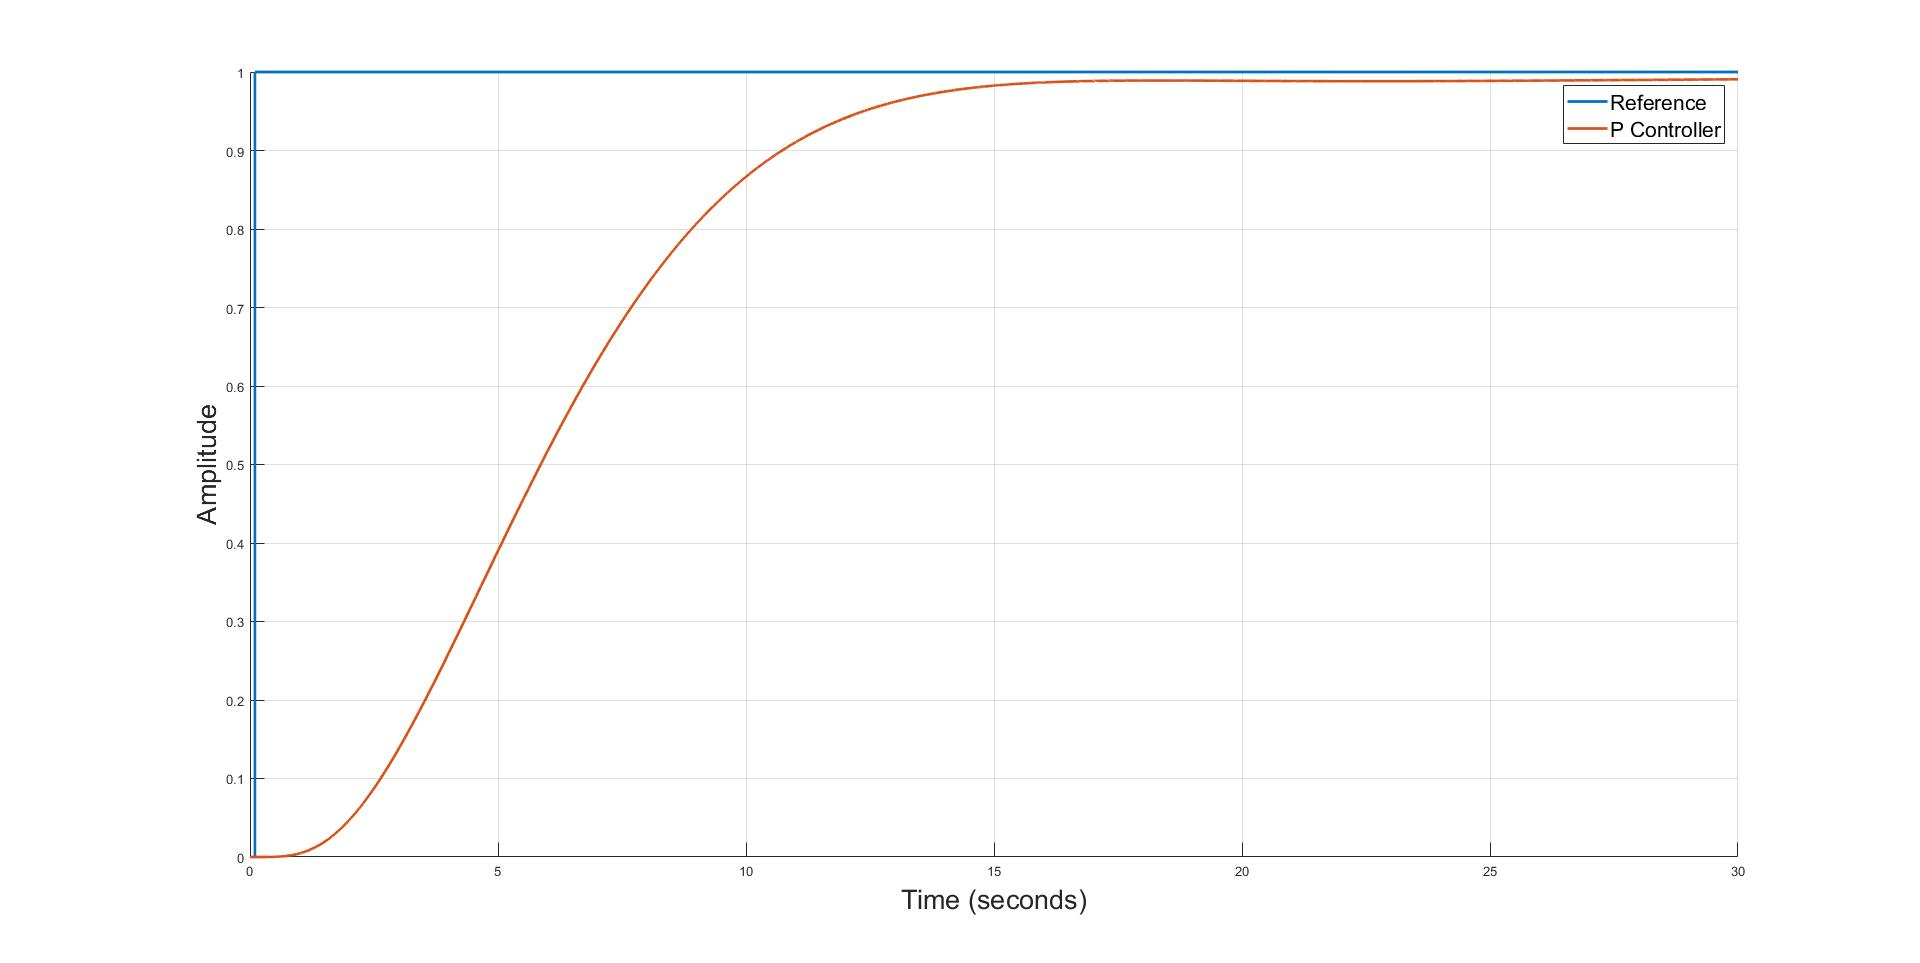
\includegraphics[height = 8cm]{../Design/Matlab/Controllers/north_position_step.jpg}
			\caption{North Position Controller -  Step Response}
			\label{IM_NorthPosControlStep}
		\end{figure}
		
		The position controller could be commanded with large step values. To prohibit commanding large velocity values a limiter is used. Figure \ref{IM_NorthPosControlLargeStep} is used to show the effect the saturation has for a large step input command. 
			
		\begin{figure}[H]
			\centering
			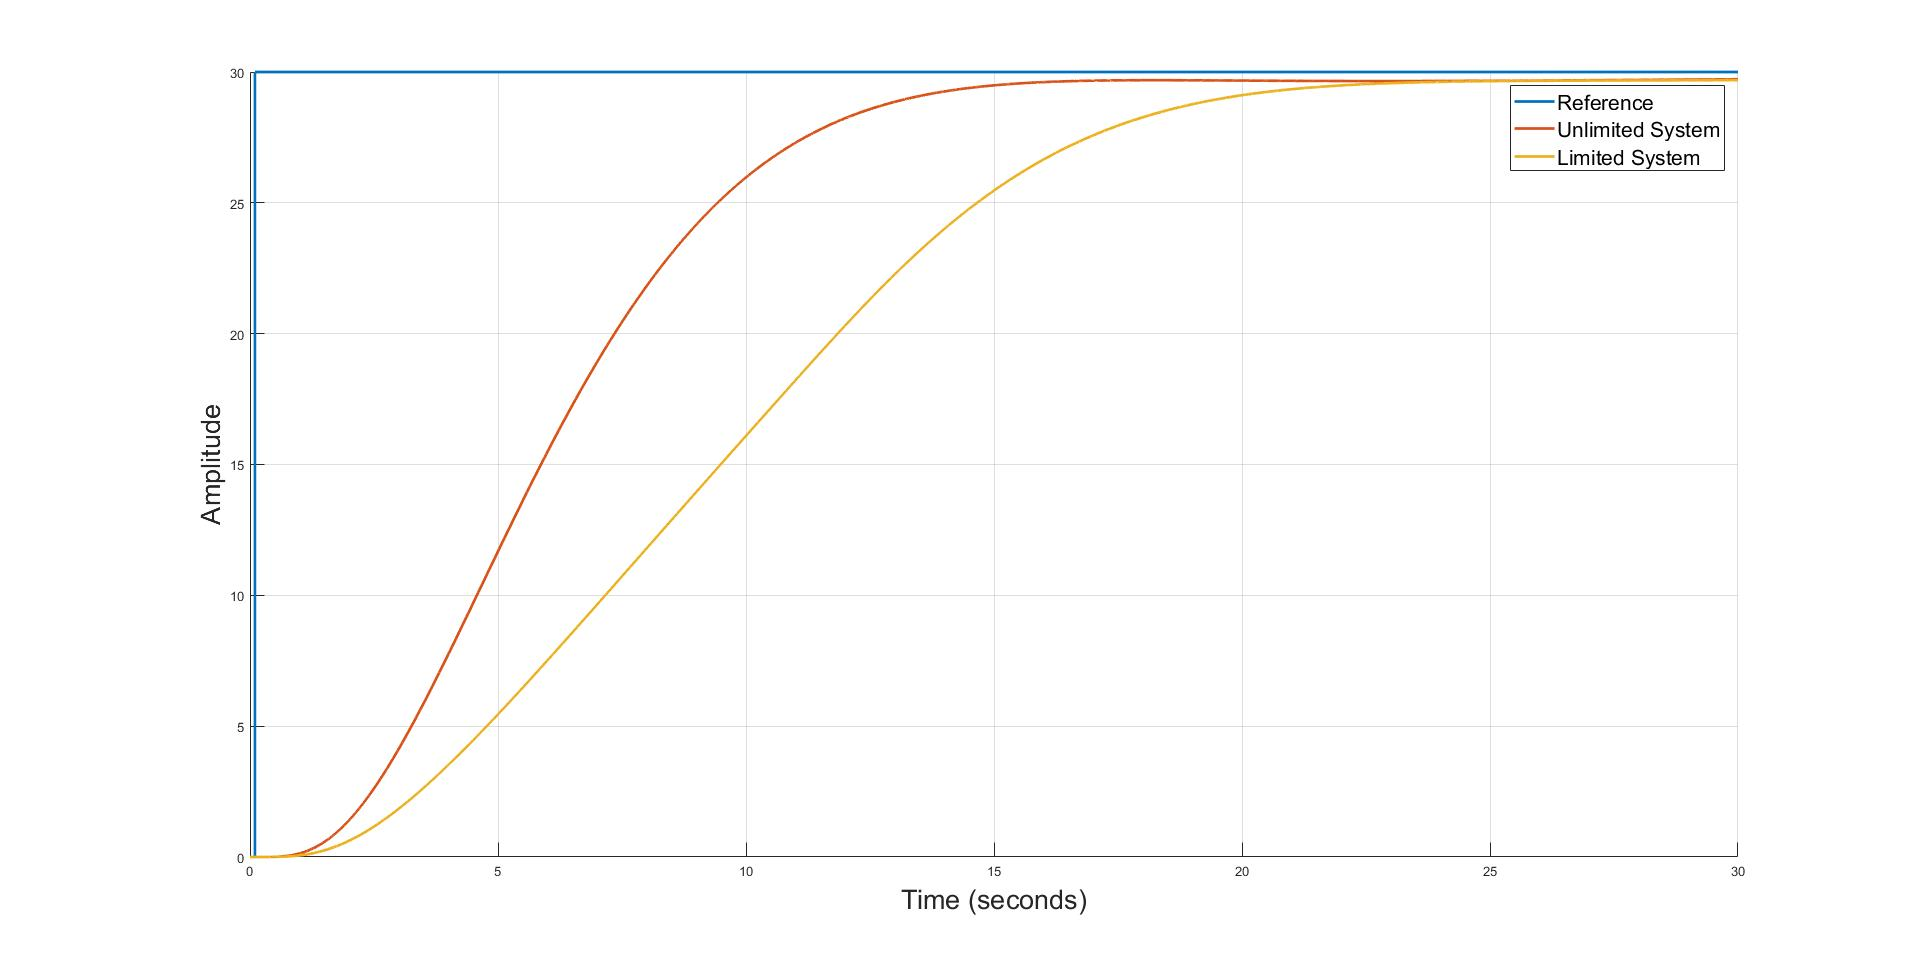
\includegraphics[height = 8cm]{../Design/Matlab/Controllers/north_pos_limit_step.jpg}
			\caption{North Position Controller -  Large Step Response With and Without a Limiter}
			\label{IM_NorthPosControlLargeStep}
		\end{figure}
				
\section{Heading Controller}
This section describes the heading controller which is responsible for aligning the craft with a desired yaw angle reference. An angle reference is given to a yaw angle controller which outputs a yaw rate reference. The inner yaw rate controller commands the yawing moment around the Z-Axis of the craft. Both the vertical and the horizontal controllers have been designed to operate independently of the heading. The craft is however, expected to fly down a narrow channel. This calls for a method of aligning the body axis of the craft with a given heading in the earth frame. This heading could be given by a higher flight planning strategy.

The craft must be able to follow a heading setpoint with zero steady state error and have a reasonably damped response. The heading controller must also be able to reject disturbances and will require an integrator in the control law. The yaw controller must also consider that the yaw torque generation has a reduction gain due to the lift to drag ratio. The design of the craft also means the yaw rate dynamics produce the lowest plant gain with the largest inertia component. The juxtaposition of a low actuation torque and lower plant gain leads to the heading controller typically being slower and exhibit less bandwidth when compared to the other controllers. Before a controller can be designed, the plant dynamics must be derived.
	
	\subsection{Yaw Rate Dynamics}
	Using Newton mechanics at near hover conditions, the yaw dynamics for the craft can be derived, the result is shown in equation \eqref{EQ_YawNewton}. $\dot{r}$ is the rotational acceleration of the craft and $N$ is the instantaneous moment experienced by the craft around the Z-Axis.
	
	\begin{equation}
	\label{EQ_YawNewton}
	\dot{r} = \dfrac{N}{I_{ZZ}}
	\end{equation}
	
	$\dot{r}$ is chosen as the output of the system with the state variable chosen as $N$. From this, the space equation for the system can be derived and is shown in \eqref{EQ_YawStateSpace1} and \eqref{EQ_YawStateSpace2}. 
	
	\begin{eqnarray}
	[\dot{N}] &=& - [\dfrac{1}{\tau}] \ [N] + [\dfrac{1}{\tau}] [\delta_\psi]\label{EQ_YawStateSpace1}\\\label{EQ_HeaveStateSpace22}
	[\dot{r}] &=& - [\dfrac{1}{I_{ZZ}}] \ [N]\label{EQ_YawStateSpace2}\\
	G(s)_{yaw} &=& \frac{\frac{1}{\tau I_{ZZ}}}{s (s + \frac{1}{\tau})}\label{EQ_YawTF}
	\end{eqnarray}
	
	From the state space representation, the transfer function for the yaw acceleration can be calculated. Integrating the result produces the transfer function for yaw rate, introducing a new pole into the system, the result is shown in \eqref{EQ_YawTF}. This plant now has two open loop poles, the first pole is due to the lag introduced by the motor rotor system, and lies at $\sigma = -\dfrac{1}{\tau} = 8$ with the second due to the integration of yaw acceleration to velocity. 
	
	\subsection{Yaw Rate Controller}	
	The yaw rate controller receives a yaw acceleration reference in radians per second (rad/s) and outputs the virtual actuator $\sigma_{\psi}$. The yawing moment is generated by air pressure on the rotors as they generate thrust, the reduction gain introduces the possibility of saturating the other controllers for large step inputs. However, as the most inner of the two heading loops, the yaw rate system limits the bandwidth of the outer yaw angle loop. The yaw rate controller must then produce enough bandwidth for the yaw angle controller, while ensuring it is not commanding thrust values above the limits described in \ref{tab:HeadRoomPercentages}. The yawing moment torque generation is also less accurately modelled and the system must exhibit high stability with large gain and phase margins. The free integrator in the yaw rate system will produce zero steady state error. The design for this controller can then be designed as a simple P controller with a non-linear saturation as shown in Figure \ref{IM_YawRateController}.
	
	\begin{figure}[H]
		\centering
		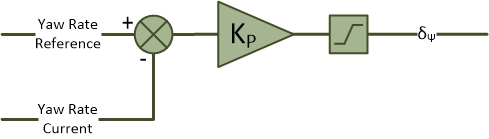
\includegraphics[height = 3.5cm]{../References/Diagrams/YawRateController.jpg}
		\caption{Yaw Rate Controller -  Control Diagram}
		\label{IM_YawRateController}
	\end{figure}
	
	The dynamic response of the proportional (P) controller is evaluated using the root locus in Figure \ref{IM_YawRateControlRoot}. The controller adds no new poles or zeros. The proportional gain is used to move the closed loops and achieve the desired bandwidth. The final closed loops poles sit at $-4 \pm 1.93$\,rad/s, the poles are slightly under damped with a damping ratio of $0.9$.
	
	\begin{figure}[H]
		\centering
		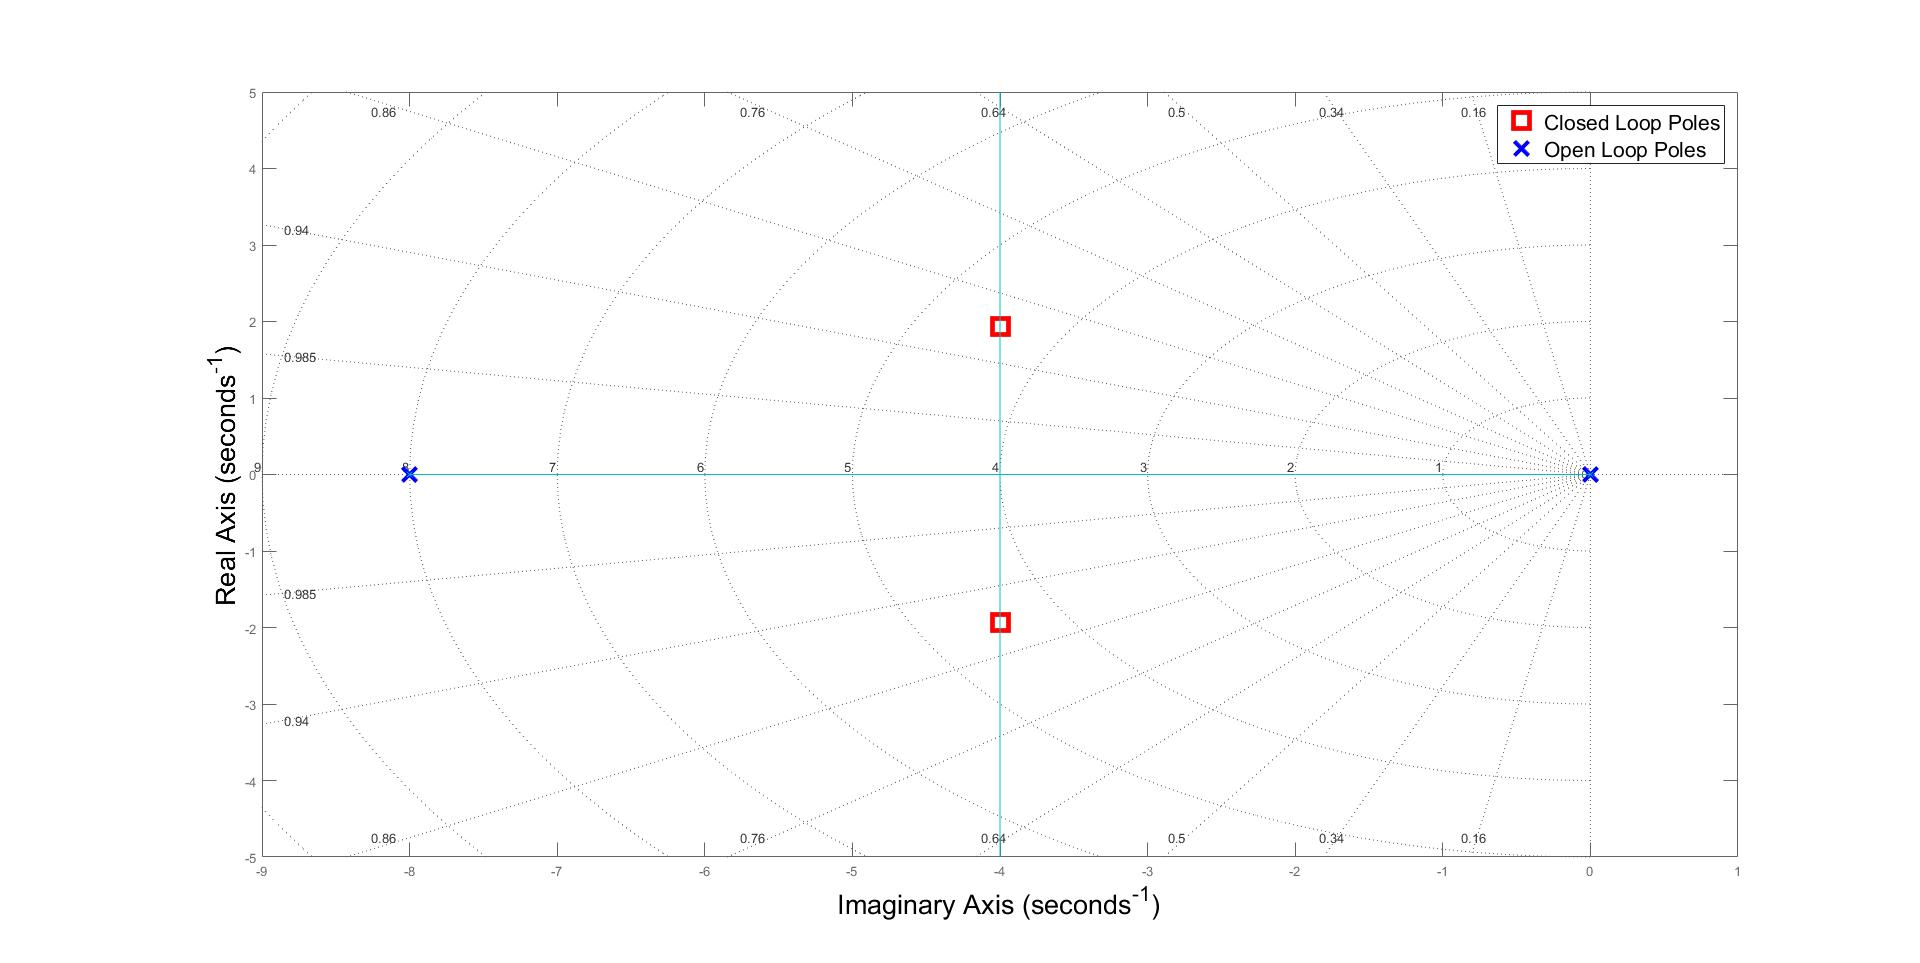
\includegraphics[height = 8cm]{../Design/Matlab/Controllers/yaw_rate_root.jpg}
		\caption{Yaw Rate Controller -  Root Locus}
		\label{IM_YawRateControlRoot}
	\end{figure}
	
	The bode plot in Figure \ref{IM_YawRateControlBode} is used to evaluate the frequency response of the system against unity feedback. As expected the controller introduces no phase change into the system. Unity feedback produces a crossover frequency of $4.99$\,rad/s which is too fast for the heading system. Reducing the gain of the system increases the phase margin to $74$\textdegree and reduces the crossover frequency by nearly half to $2.37$\,rad/s.
	
	\begin{figure}[H]
		\centering
		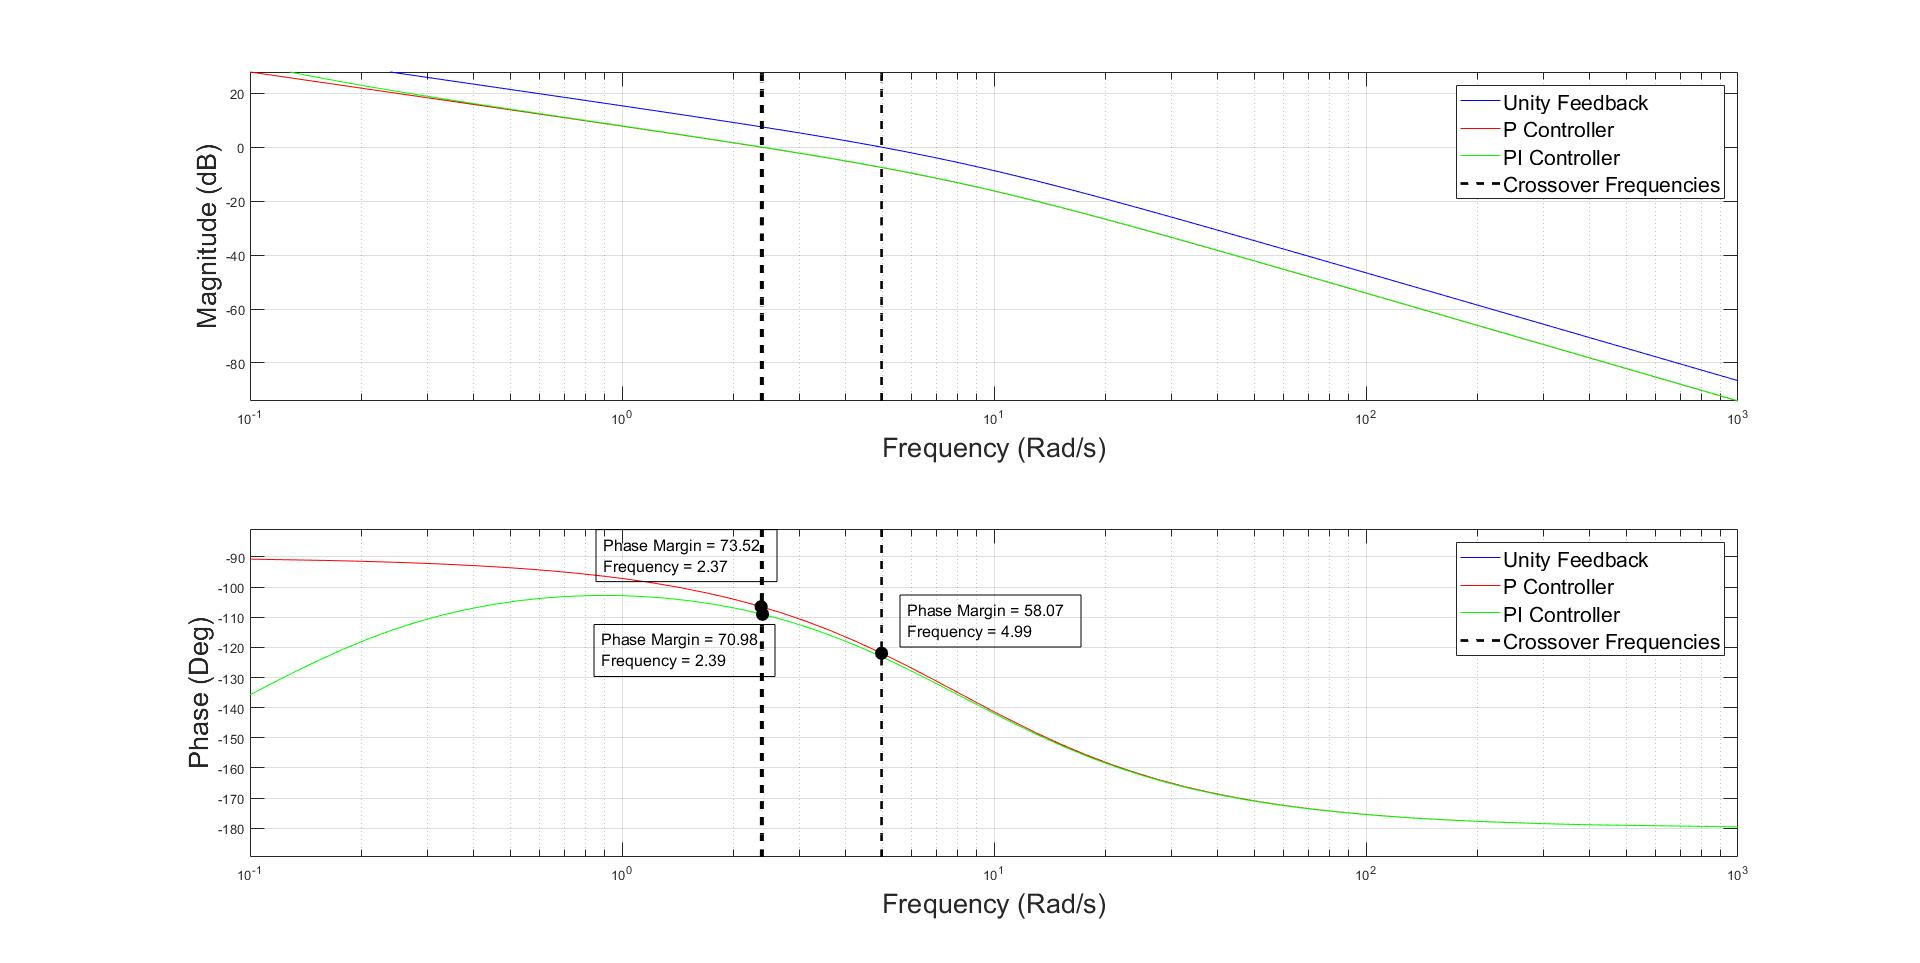
\includegraphics[height = 8cm]{../Design/Matlab/Controllers/yaw_rate_bode.jpg}
		\caption{Yaw Rate Controller -  Bode Plots}
		\label{IM_YawRateControlBode}
	\end{figure}
	
		\subsubsection{Yaw Rate Controller Discussion}
		The controller increases stability in the system and produces the step response shown in Figure \ref{IM_YawRateStep}. The system has a $5\% $ settling time of $0.9s$ and negligible overshoot. The maximum thrust commanded per motor using this system is $0.26$\,N, which falls in the limits of this system. The low gain of the system makes this system susceptible to disturbances and calls for an outer angle loop. 
					
		\begin{figure}[H]
			\centering
			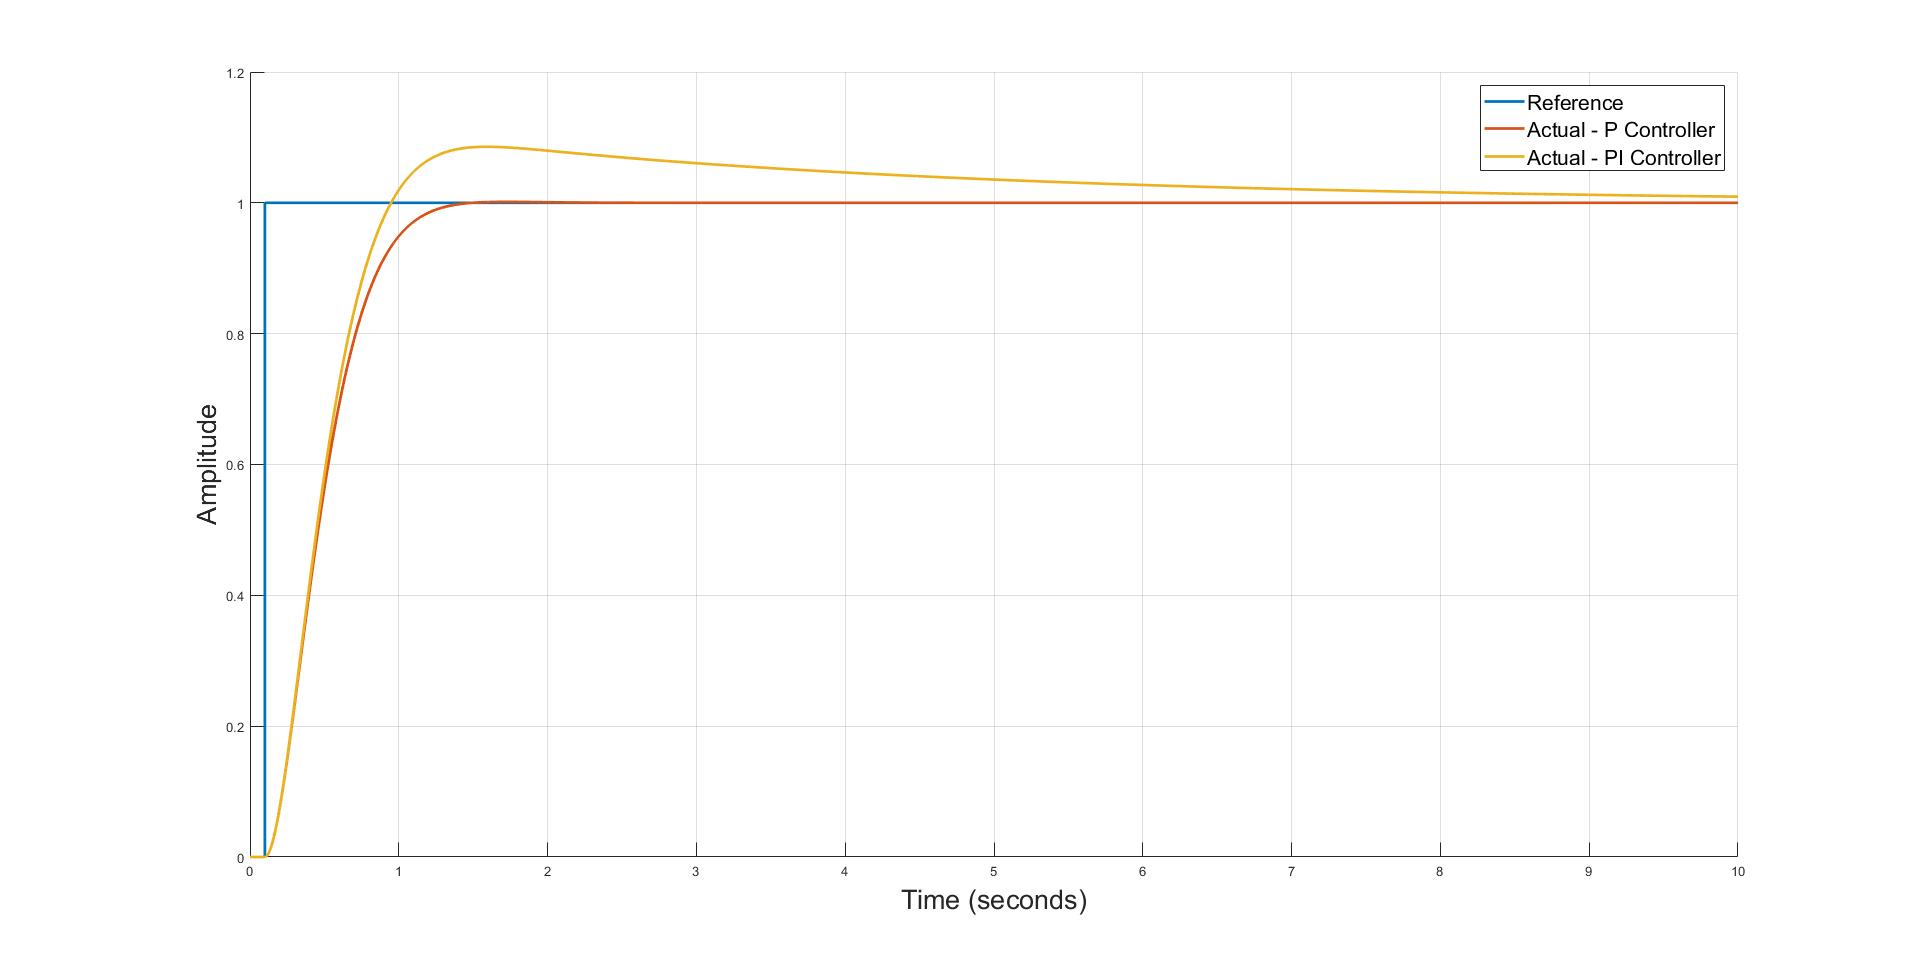
\includegraphics[height = 8cm]{../Design/Matlab/Controllers/yaw_rate_step.jpg}
			\caption{Yaw Rate Controller -  Step Responses}
			\label{IM_YawRateStep}
		\end{figure}
		
	\subsection{Yaw Angle Controller}\label{SSECT_YawAngleController}	
	The yaw angle controller receives a heading reference in radians and outputs a yaw angle rate reference in radians per second to the inner rate controller as shown in Figure \ref{IM_YawAngleLoop}. This controller is limited by the inner loop and must ensure significant bandwidth between the inner and outer loops. The system must be able to reject disturbances and requires an integrator in the system. The system must be reasonably damped with limited overshoot.

	\begin{figure}[H]
		\centering
		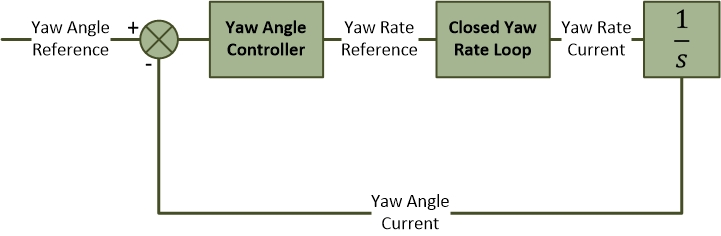
\includegraphics[height = 3.5cm]{../References/Diagrams/YawAngleLoop.jpg}
		\caption{Yaw Angle PI Controller -  Control Diagram}
		\label{IM_YawAngleLoop}
	\end{figure}
	
	Initially a Proportional Integral (PI) controller was considered as shown in Figure \ref{IM_YawAngleController}. The proportional gain is used to move the closed loop poles and achieve the desired bandwidth. The integral term is introduced to account for expected disturbances as well as measurement errors in the rate loop. The PI controller adds a new zero and a new pole into the system. 
	
	\begin{figure}[H]
		\centering
		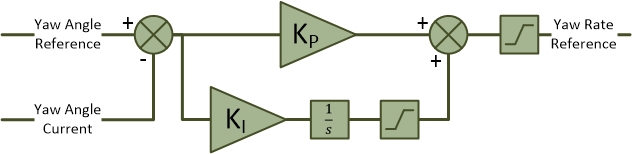
\includegraphics[height = 3.5cm]{../References/Diagrams/YawAngleControllerPI.jpg}
		\caption{Yaw Angle PI Controller -  Control Diagram}
		\label{IM_YawAngleController}
	\end{figure}
	
	The second scheme was designed as a Proportional Integral Derivative (PID) controller as shown in Figure \ref{IM_YawAngleControllerPID}, the differential term is introduced to increase the phase of the system and adds an additional zero. The differential command is fed through a low pass filter to reduce noise on the command. As shown both controllers contain non linear elements that are not considered during the linear design. The components excluded during the analysis are all the limiters as well as the low pass filter seen in the differentiator portion of the PID leg.
	
	\begin{figure}[H]
		\centering
		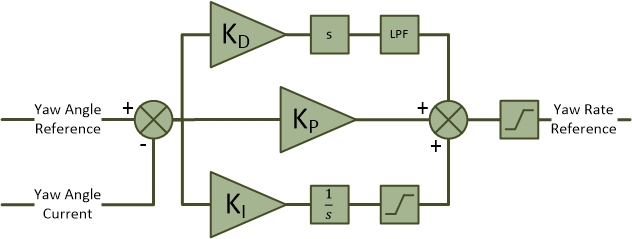
\includegraphics[height = 5.5cm]{../References/Diagrams/YawAngleControllerPID.jpg}
		\caption{Yaw Angle PID Controller -  Control Diagram}
		\label{IM_YawAngleControllerPID}
	\end{figure}

	The dynamic response of each system can be evaluated using the root loci diagrams seen in Figure \ref{IM_YawAngleControlRoot}. The plant has two open loop poles at the closed loop yaw rate pole locations, as well as a new pole at the origin introduced by the mathematical relationship between speed and position. Both controllers introduce one new open loop pole at the origin and at least one zero. The PID controller introduces an additional zero into the system.  
	
	The final closed loop pole positions for the PI controller all lie on the imaginary axis and are located at $-3.62$, $-3.26$, $-0.88$ and $-0.25$. The PID controller has a dominant complex pair of closed loop poles at $-0.52 \pm 0.51 i$ with the other non-dominant closed loop pole pair sitting at $-3.48 \pm 2.54 i$. The PI controller has critically damped dominant poles where as the dominant poles for the PID controller are under damped with a damping ratio of $0.71$.
	
	\begin{figure}[H]
		\centering
		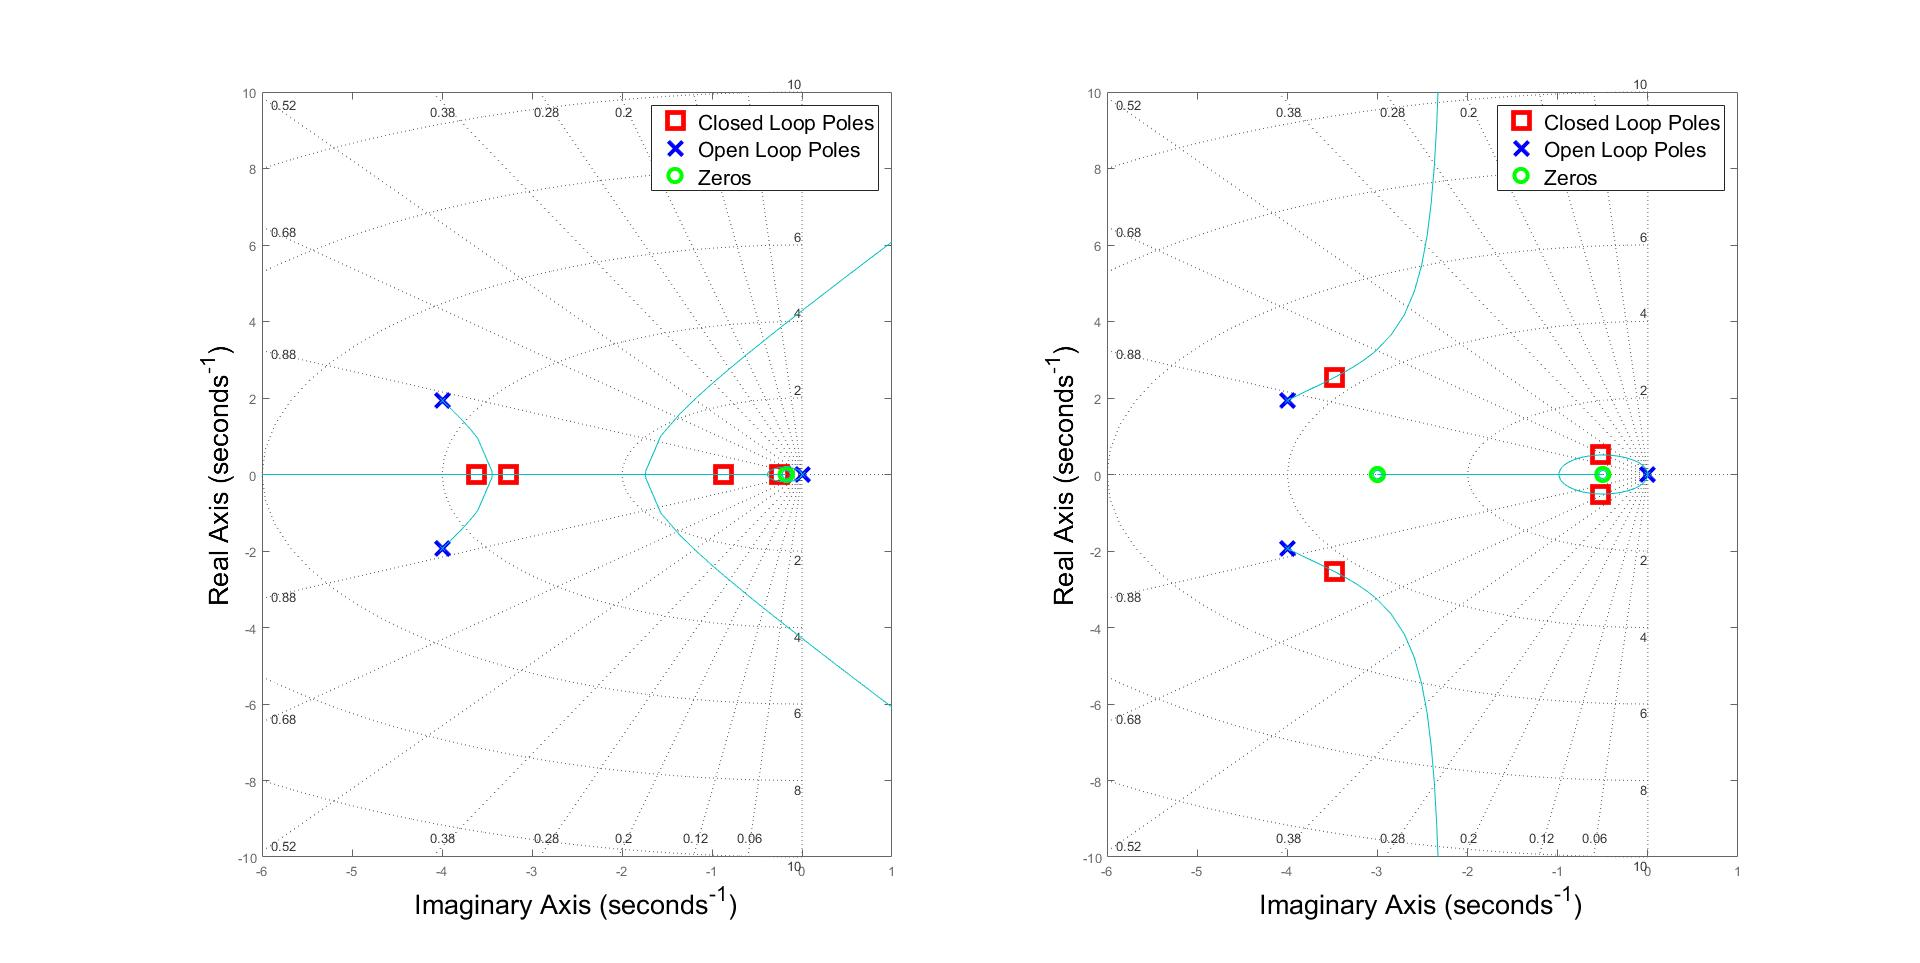
\includegraphics[height = 8cm]{../Design/Matlab/Controllers/yaw_angle_root.jpg}
		\caption{Yaw Angle Controller -  Root Locus (Left:PI, Right:PID)}
		\label{IM_YawAngleControlRoot}
	\end{figure}
	
	The frequency response of both systems is evaluated next. Using the open loop bode plots shown in Figure \ref{IM_YawAngleControlBode}, unity feedback is compared with a PI and PID controller. The first zero in both cases is placed close to the origin to limit the effect the new zero has on the system. The PID controller's second zero is placed to increase the phase of the system, allowing for more bandwidth in each leg of the controller. This additional phase allows for larger and more aggressive disturbance rejection, but will result in larger setpoints for the inner yaw rate loop.
	
	The gain of each system has similar bandwidth around the cross over point. The extra zero in the PID controller reduces the gradient of the gain slope off and increases the total phase of the system. The PID controller exhibits the second largest phase margin of $61$\textdegree\ which is found at $1.12$\,rad/s, the fastest of the three crossover frequencies. The PI controller achieves the desired bandwidth and has the slowest crossover frequency of $0.75$\,rad/s, this however relates to a lower phase margin of $59$\textdegree. The final crossover frequency of the yaw rate system was $2.37$\,rad/s, resulting in a ratio with the PID controller of $2.12$ and a ratio of $3.16$ with the PI controller. A larger ratio implies less risk of attenuation for the outer loop.
	
	\begin{figure}[H]
		\centering
		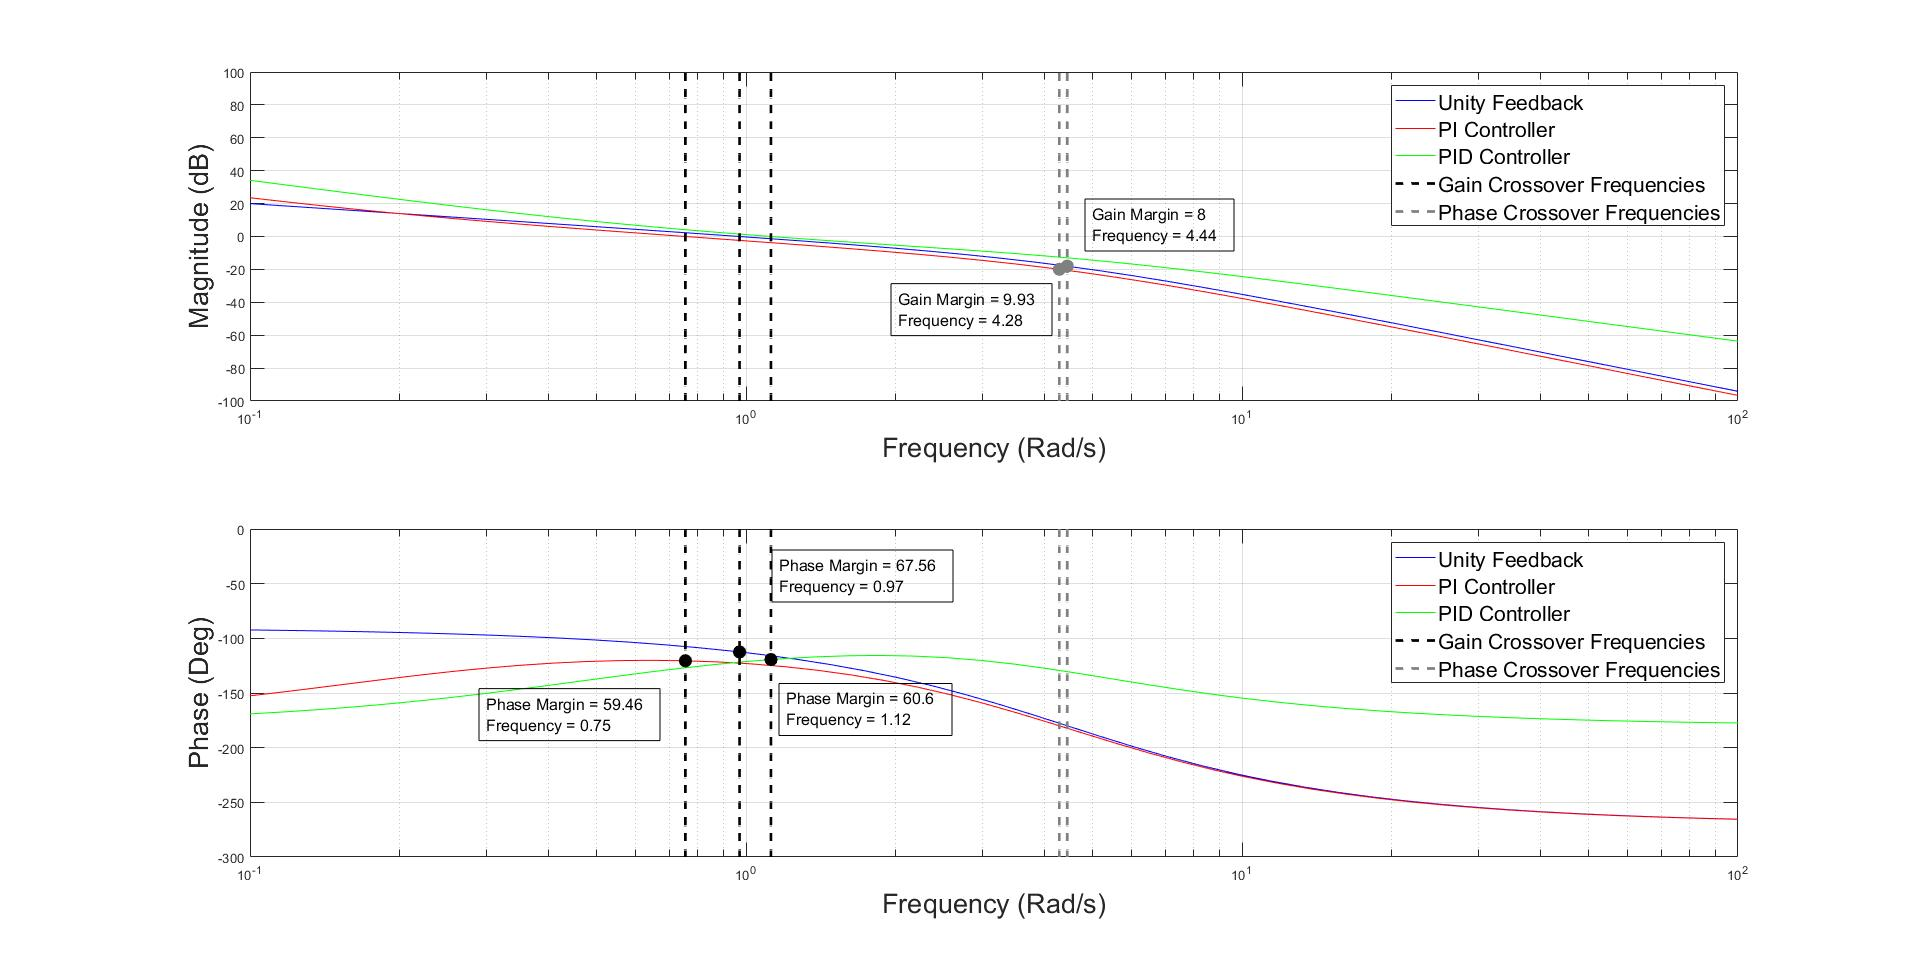
\includegraphics[height = 8cm]{../Design/Matlab/Controllers/yaw_angle_bode.jpg}
		\caption{Yaw Angle Controller -  Bode Plots}
		\label{IM_YawAngleControlBode}
	\end{figure}
	
		\subsubsection{Yaw Angle Controller Discussion}	
		Each controller was added to the non-linear simulation and evaluated in the time domain including the non linearities previously unconsidered. Figure \ref{IM_YawAngleStep} shows the results of both controllers with and without the limits as well as the additional low pass filter on the differential gain. The PID controller without any limits or low pass filtering had a $5$ \% settling time of $6.37s$, adding in the limits and filter decreases that time to $4.9s$. The PI controller had a settling time of $10.3s$ with no limits which was decreased to $8.8s$ by the addition of the limit on the integrator.
		
		All three systems exhibit some overshoot. The limiters must be carefully chosen to reduce overshoot while also still allowing for substantial disturbance rejection. The linear PI and PID systems produce overshoot of $17$\% and $29$\% respectively. The limits for the integrators on both systems was set to $\pm 0.1$\,rad/s. This limit also becomes the maximum offset this controller can successfully correct for. Both systems had significant overshoot reduction, the PI controller now only had an $12$\% overshoot, with the limited PID system showing only $6$\% overshoot. 
				
		\begin{figure}[H]
			\centering
			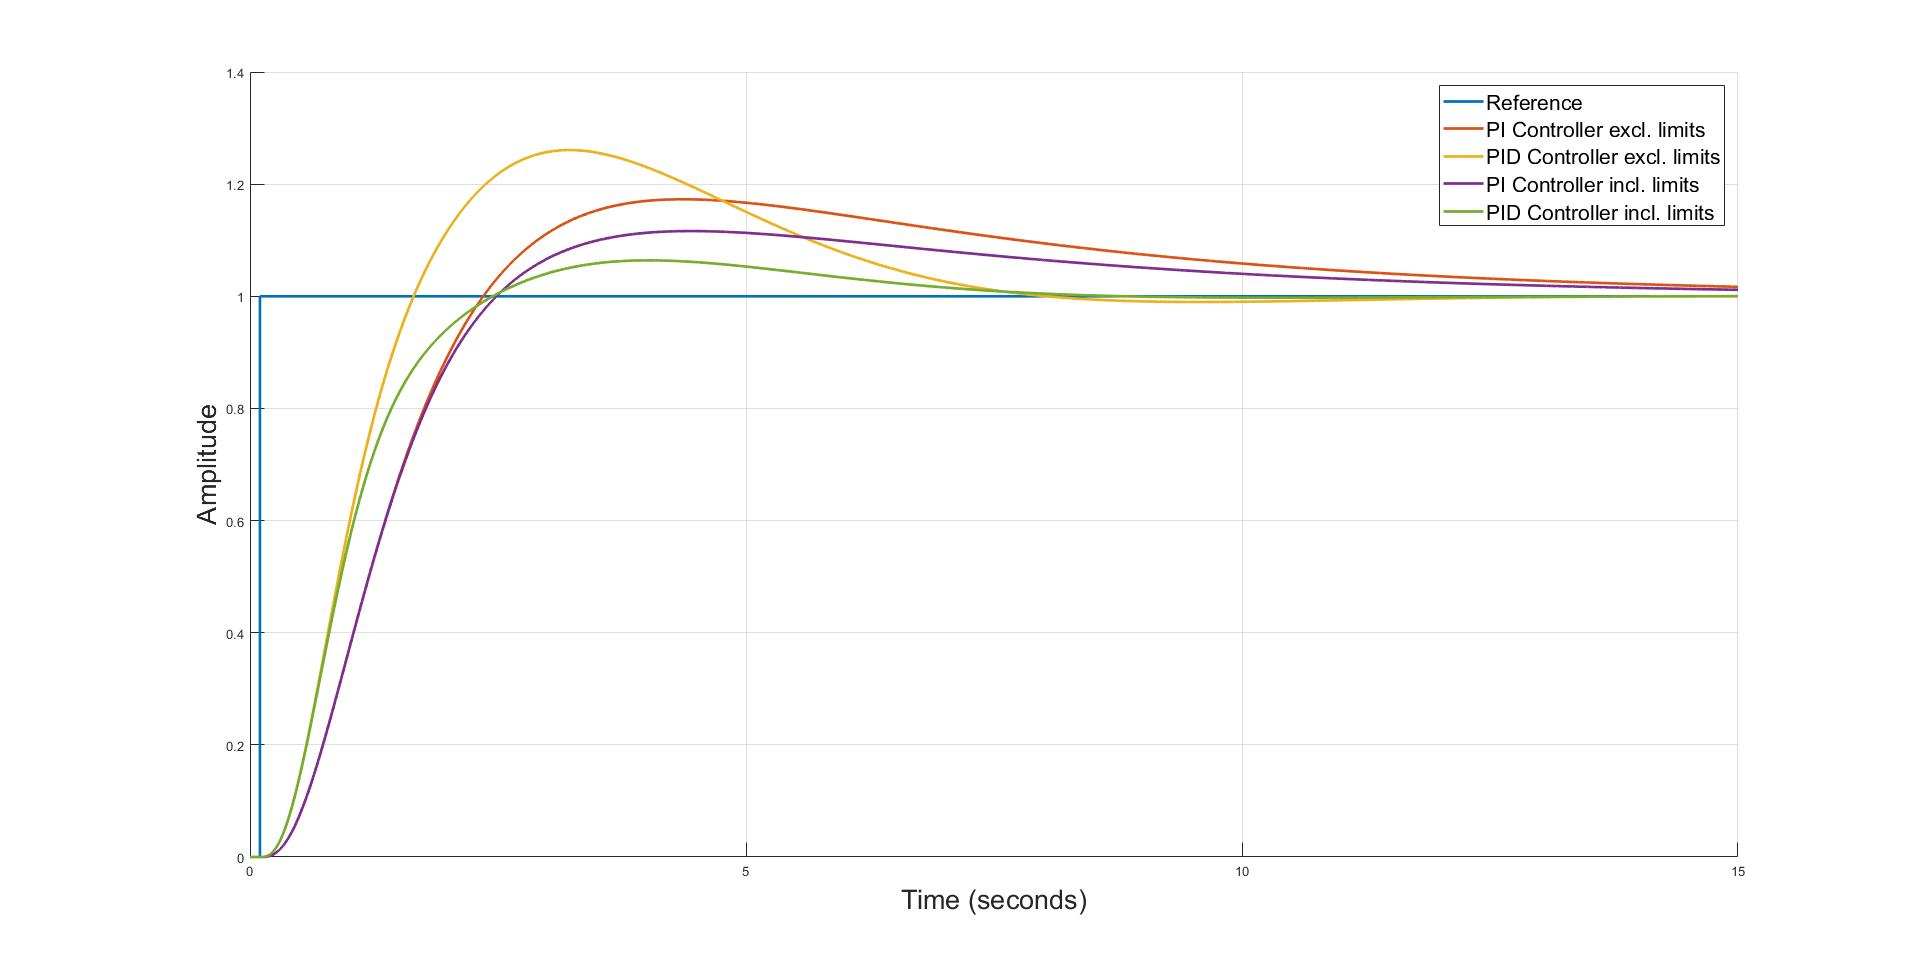
\includegraphics[height = 8cm]{../Design/Matlab/Controllers/yaw_angle_step_both_limits.jpg}
			\caption{Yaw Angle Controller -  Step Responses}
			\label{IM_YawAngleStep}
		\end{figure}
		
		As mentioned the limits introduce the maximum disturbance rejection capability of each system. Figure \ref{IM_YawAngleStepBoth} shows how each limited system handles a measurement offset of $0.1$\,rad/s in the yaw rate loop.
		
		\begin{figure}[H]
			\centering
			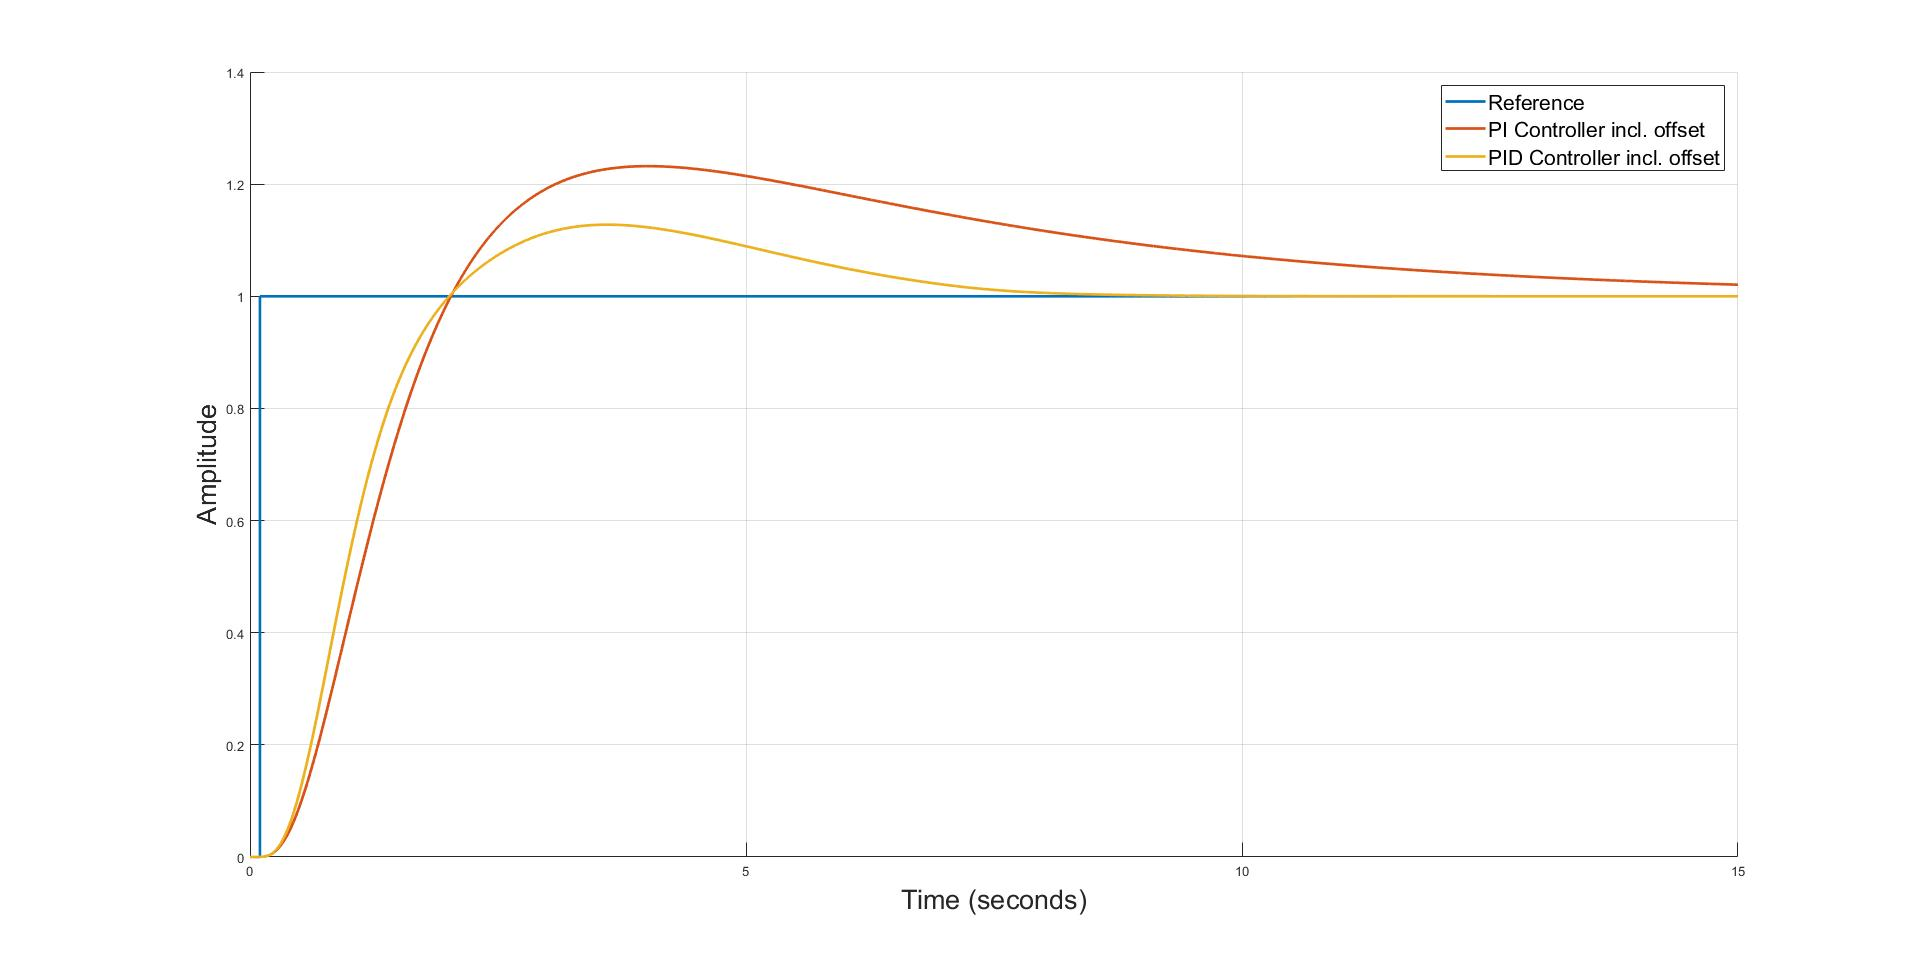
\includegraphics[height = 8cm]{../Design/Matlab/Controllers/yaw_angle_step_both_dist.jpg}
			\caption{Yaw Angle Controller -  Step Responses Including Inner Loop Measurement Offset}
			\label{IM_YawAngleStepBoth}
		\end{figure}
		
		The final consideration is the impulse each system creates for the yaw rate controller, Figure \ref{IM_YawAngleImpulse} demonstrates both limited systems impulse responses. As seen the PID controller commands a larger initial setpoint, more than double that of the PI controller.    
		
		\begin{figure}[H]
			\centering
			\includegraphics[height = 8cm]{../Design/Matlab/Controllers/yaw_angle_impulse.jpg}
			\caption{Yaw Angle Controller -  Impulses}
			\label{IM_YawAngleImpulse}
		\end{figure}
		
		The PI controller is chosen as the final controller implementation. 
		